\documentclass[10pt]{report}
\usepackage{fancyhdr, amsmath, amsthm, amssymb, tikz, setspace, hyperref}
\usepackage[font=scriptsize]{subcaption}
\usepackage[margin=0.5in, top=0.8in,bottom=0.8in]{geometry}
\usepackage[version=3]{mhchem}
\newcommand{\scinot}[2]{#1\times 10^{#2}}
\newcommand{\bra}[1]{\left<#1\right|}
\newcommand{\ket}[1]{\left|#1\right>}
\newcommand{\dotp}[2]{\left<#1\left.\right|#2\right>}
\newcommand{\rd}[2]{\frac{d#1}{d#2}}
\newcommand{\pd}[2]{\frac{\partial #1}{\partial#2}}
\newcommand{\norm}[1]{\left|\left|#1\right|\right|}
\newcommand{\ptd}[2]{\frac{\partial^2 #1}{\partial#2^2}}
\newcommand{\rtd}[2]{\frac{d^2#1}{d#2^2}}
\newcommand{\tensor}[1]{\overleftrightarrow{#1}}
\newcommand{\curl}[0]{\vec{\nabla}\times}
\newcommand{\pvec}[1]{\vec{#1}^{\,\prime}}
\newcommand{\grad}[0]{\vec{\nabla}}
\let\Re\undefined
\let\Im\undefined
\DeclareMathOperator{\Re}{Re}
\DeclareMathOperator{\Im}{Im}
\renewcommand{\div}[0]{\vec{\nabla}\cdot}
\newcommand{\expvalue}[1]{\left<#1\right>}
\newcommand{\abs}[1]{\left|#1\right|}
\usepackage[labelfont=bf, font=scriptsize]{caption}
\everymath{\displaystyle}

\begin{document}

%\doublespace
\pagestyle{fancy}
\rhead{Yubo Su - Ph106}
%\setlength{\headheight}{15pt}

\title{Ph106c - Sunil Golwala - DWN107 TTh 1030-12}
\author{Yubo Su}
\date{ }

\maketitle

\tableofcontents

\chapter{Key Concepts}

\begin{itemize}
    \item Useful BCs
        \begin{itemize}
            \item $\hat{n}\cdot \left[ \epsilon_2\vec{\nabla}V_2 - \epsilon_1\vec{\nabla}V_1 \right] = \sigma_f$
            \item $V$ is continuous.
            \item $\rho_b= -\frac{\epsilon - \epsilon_0}{\epsilon}\rho_f$ inside the volume.
        \end{itemize}
    \item For linear homogeneous dielectric $U = \frac{\epsilon_0}{2}\int\limits_{\mathcal{V}}^{}E^2\;d\tau'$.
    \item Introducing dielectric to existing $\vec{E}$ yields energy $U = -\frac{1}{2}\int\limits_{\mathcal{V}}^{}d\tau'\;\vec{P}\cdot \vec{E}$.
    \item Lorentz force law $\vec{F} = q(\vec{E} + \vec{v}\times \vec{B})$.
    \item Continuity equation $\vec{\nabla}\cdot\vec{J} = -\pd{\rho}{t}$.
    \item Biot-Savart Law 
        $$\vec{B}(\vec{r}) = \frac{\mu_0}{4\pi}\int\limits_{}^{}dl'\;\vec{I}(\pvec{r}) \times \frac{\vec{r} - \pvec{r}}{\abs{\vec{r} - \pvec{r}}^3} = \vec{\nabla} \times \frac{\mu_0}{4\pi}\int\limits_{V}^{}d\tau'\;\frac{\vec{J}(\pvec{r})}{\abs{\vec{r} - \pvec{r}}}$$
    \item Ampere's Law (Integral form $\int\limits_{C}^{}d\vec{l}\cdot\vec{B}(\vec{r}) = \mu_0 I_{enc}$)
        $$\vec{\nabla}\times\vec{B}(\vec{r}) = \mu_0\vec{J}(\vec{r})$$
    \item Vector potential $\vec{B} = \vec{\nabla} \times \vec{A}$ under Coulomb gauge $\vec{\nabla}\cdot\vec{A} = 0$ is
        $$\vec{A}(\vec{r}) = \frac{\mu_0}{4\pi}\int\limits_{V}d\tau'\;\frac{\vec{J}(\pvec{r})}{\abs{\vec{r} - \pvec{r}}}$$
    \item BCs on $\vec{B}$ and derivatives of $\vec{A}$ are
        \begin{align}
            \hat{n} \cdot\left[ \vec{B}_2 - \vec{B}_1 \right] &= 0 &\hat{n}\times\left[\vec{B}_2 - \vec{B}_1\right] &= \mu_0\vec{\kappa}\\
            \hat{n}\cdot\vec{\nabla}\left[ \vec{A}_2 - \vec{A}_1\right] &= \mu_0 \vec{\kappa} & \hat{s}\cdot \vec{\nabla}\left[ \vec{A}_2 - \vec{A}_1 \right] &= 0
        \end{align}
        $\vec{A}$ is continuous across boundaries under Coulomb Gauge.
    \item Force, torque, energy of dipoles
        \begin{align}
            \vec{F} &= \vec{\nabla}(\vec{m}\cdot \vec{B})&
            \vec{N} &= \vec{m}\times \vec{B}&
            U &= -\vec{m}\cdot \vec{B}
        \end{align}
    
    \item For $\vec{J}_b = \vec{\nabla} \times \vec{M}$ and $\vec{K}_b = \vec{M}\times \hat{n}$ bound volume and surface current densities respectively we have
        $$\vec{A} = \frac{\mu_0}{4\pi}\left[ \int\limits_{V}^{}d\tau\;\frac{\vec{\nabla}\times \vec{M}}{\abs{\vec{r} - \pvec{r}}} + \int\limits_{S}^{}\frac{\vec{M}\times d\vec{S}}{\abs{\vec{r} - \pvec{r}}}\; \right]$$
    \item Auxiliary field $\vec{H} = \frac{\vec{B}}{\mu_0} - \vec{M}$ exhibits $\vec{\nabla}\times \vec{H} = \vec{J}_f$. Obeys Ampere's Law integral form for $\vec{H}, \vec{J}_f$, but careful to check for $\vec{\nabla} \cdot \vec{M}$. Linear, $\mu\vec{H} = \vec{B}$. 
    \item BCs on $\vec{H}$
        \begin{align}
            \hat{n}\cdot \left[ \vec{H}_2 - \vec{H}_1 \right] &= -\hat{n}\cdot \left[ \vec{M}_2 - \vec{M}_1 \right]\\
            \hat{n} \times \left[ \vec{H}_2 - \vec{H}_1 \right] &= \vec{K}_f
        \end{align}
    \item Three ways/cases to solve BVPs in magnetostatics
        \begin{itemize}
            \item $\nabla^2\vec{A} = -\mu \vec{J}_f$ is the analogue of Poisson's equation for linear, homogeneous materials. 
            \item If $\vec{J}_f = 0$ note $\vec{\nabla} \times \vec{H} = 0$ so we can use a magnetostatic scalar potential $\vec{H} = -\vec{\nabla}V_M$ with $\nabla^2 V_m = 0$.
            \item Hard ferromagnetic regime: here, nonlinear ($\vec{B} \neq \mu \vec{H}$) with fixed $\vec{M}$, $\vec{J}_f = 0$. Can use $\nabla^2 V_m = -\vec{\nabla} \cdot\vec{M}$. Note will need surface charge term $\sigma_M = \hat{n} \cdot \vec{M}$ along surfaces.
        \end{itemize}
    \item Note that literally anything can be expanded in terms of the $Y_{lm}$ and anything azimuthally symmetric can be expanded in terms of the $P_l$; this is not exclusive to the few BVP cases we've studied (notably helpful for $\Phi_m$ magnetoscalar potentials)! Thus, oftentimes problems can be solved by going to $Y_{lm}, P_l$ (notably $\abs{\vec{r} - \pvec{r}}^{-1}$ can be expanded) and orthogonality can solve us many a problem.
\end{itemize}
{\large
    \textbf{Electrodynamics!!}
}
\begin{itemize}
    \item Ohm's Law is $\vec{J} = \sigma \vec{E}$ or $V = IR$.
    \item Lenz's Law that $\varepsilon$ in Faraday's Law is such that it opposes change in flux.
    \item Faraday's Law $\varepsilon = -\rd{\Phi}{t}, \vec{\nabla} \times \vec{E} = -\rd{\vec{B}}{t}$
    \item Mutual inductance $M_{21} = \oint\limits_{C_2, C_1}\frac{d\vec{l}_2\cdot d\vec{l}_2}{\abs{\vec{r}_2 - \vec{r}_1}}$, useful because $\varepsilon_2 = -M_{21}\rd{I_1}{t}$.
    \item Energy stored in $B$ field, energy of dimagnetic in external field is
        \begin{align}
            E &= \frac{1}{2\mu_0}\int\limits_{\mathcal{V}}^{}\abs{B}^2\;d\tau & U_2 - U_1 &= \frac{1}{2}\int\limits_{\mathcal{V}_2}^{}d\tau\;\left( \frac{1}{\mu_1} - \frac{1}{\mu_2} \right)\vec{B}_2 \cdot \vec{B}_1
        \end{align}
    \item In presence of currents, Faraday's Law looks more like
        $$\vec{\nabla} \times \vec{B} = \mu_0 \vec{J} + \mu_0\epsilon_0 \pd{\vec{E}}{t}$$
    \item The forms of Gauss's/Ampere's Law for 
        \begin{align}
            \vec{\nabla} \cdot \vec{D} &= \rho_f & \vec{\nabla} \times \vec{H} = \vec{J}_f + \pd{\vec{D}}{t}
        \end{align}
    \item Poynting Theorem is $\rd{}{t} E = -\vec{\nabla} \cdot \vec{S}$ with $E$ the sum of the mechanical and electromagnetic energy, is a continuity equation of energy.
    \item Maxwell stress tensor looks like
        \begin{align}
            \rd{}{t} E &= -\vec{\nabla} \cdot \vec{S}\\
            \mathbf{T} &= \sum_{i,j}^{3}T_{ij}\hat{r}_i \hat{r}_j \\
            T_{ij} &= \epsilon_0\left( E_iE_j - \frac{1}{2}\delta_{ij}E^2 \right) + \frac{1}{\mu_0}\left( B_i B_j - \frac{1}{2}\delta_{ij}B^2 \right)
        \end{align}
        leading to a continuity equation $\rd{}{t}\left( \vec{p}_m + \vec{g} \right) = \vec{\nabla} \cdot \mathbf{T}$ with $\vec{g} = \mu_0 \epsilon_0 \vec{S}$, which looks like a Newton's Second Law. Indeed, $T_{ij}$ is the force in the $i$th direction for an area element in the $j$th direction. This is a continuity equation of momentum of EM waves.
    \item Boundary conditions between two linear media for EM waves
        \begin{align}
            \hat{n} \cdot \epsilon_1 \vec{E}_1 &= \hat{n} \cdot \epsilon_2 \vec{E}_2 & \hat{n} \cdot \vec{B}_1 &= \hat{n}\cdot \vec{B}_2\\
            \hat{s} \cdot \vec{E}_1 &= \hat{s} \cdot \vec{E}_2 & \hat{s} \cdot \frac{\vec{B}_1}{\mu_1} &= \hat{s} \cdot \frac{\vec{B}_2}{\mu_2}
        \end{align}
    \item EM waves attenuate in conductors, can be modelled as a complex $\vec{k}_t$ transmitted wavevector. 
    \item Transmission lines obey
        \begin{align}
            \ptd{I}{z} &= \mathcal{L}\mathcal{C}\ptd{I}{t} & \ptd{\Delta V}{z} &= \mathcal{LC}\ptd{\Delta V}{t}
        \end{align}
        and has characteristic impedance $Z_{\mathcal{LC}} = \sqrt{\frac{\mathcal{L}}{\mathcal{C}}}$.
    \item GG, too much material towards the end of class
\end{itemize}

\chapter{4/1/14 --- BVPs with polarized materials, energy/forces/torques on dielectrics}

Feel better about yourself, the final had mean $17.4 \pm 5$ and median $18.5$. Let's jump right back into it.

Recall that for polarizable materials we have some dipole moment per molecule or atom $\vec{p}$ and for linear media is related to the applied field by $\vec{p} = \alpha \vec{E}$ with $\alpha$ a constant the polarizability. Then $\vec{P} = n\vec{p}$ the polarization density, with $n$ number of dipoles per volume. Then we obtain a bound surface charge density $\sigma_b = \hat{n}\cdot \vec{P}$ at the boundary and a bound charge volume density $\rho_b = -\vec{\nabla}\cdot \vec{P}$. 

We then defined something called the displacement field $\vec{D} = \epsilon_0\vec{E} + \vec{P}$ that obeys Gauss's law for free charges $\vec{\nabla}\cdot \vec{D} = \rho_f$ but in general $\vec{\nabla}\times\vec{D} = \vec{\nabla}\times\vec{P} \neq 0$. Boundary conditions then yield $\hat{n}\cdot[\vec{D}_2 - \vec{D}_1] = \sigma_f$ and $\hat{s} \cdot [\vec{D}_2 - \vec{D}_1] =\hat{s} \cdot [\vec{P}_2 - \vec{P}_1]$ with the surface normal and tangent.

Then for linear homogeneous dielectric we can make simplifying rewritings $\vec{P} = \epsilon_0\chi_e\vec{E}$ with $\chi_e$ the susceptibility. Then we can write $\vec{D} = \epsilon\vec{E}$ with $\epsilon = \epsilon_0(1 + \chi_e)$. Usually dielectrics will yield most easily to application of Gauss's law with $\vec{E}$ which is continuous at boundaries.

Let's examine the linear, homogeneous case first. Then we start with
\begin{align}
    \rho_b &= -\vec{\nabla}\cdot \vec{P} = -\vec{\nabla}\cdot\left( \frac{\epsilon - \epsilon_0}{\epsilon}\vec{D} \right)\\
    &= -\frac{\epsilon - \epsilon_0}{\epsilon}\rho_f
\end{align}

Then within the volume the bound charge is simply proportional to the free charge. More importantly for us, when $\rho_f = 0$ we can apply Laplace's equation to $\vec{P}$.

We also need more boundary conditions, so 
\begin{align}
    \hat{n}\cdot [\vec{D}_2 - \vec{D}_1] &= \sigma_f\\
    \hat{n}\cdot \left[ \epsilon_2\vec{\nabla}V_2 - \epsilon_1\vec{\nabla}V_1 \right] &= \sigma_f
\end{align}

Recall that $V$ is always continuous, and this will help us solve problems. We will take a different example from Griffiths. Let's exhibit a dielectric in a uniform field with spherical cavity with $\epsilon_0$ inside.

Our boundary conditions then of course have 
\begin{enumerate}
    \item $V(r \to \infty) = -E_0rP_1(\cos\theta)$ for the applied field. 
    \item Since there is then no free charge at the interface we also have $\epsilon_0\pd{V_<}{r}\Big|_{r = R} = \epsilon \pd{V_>}{r}\Big|_{r = R}$. 
    \item We also of course have continuity of potential $V_<(R,\theta,\phi) = V_>(R, \theta, \phi)$.
    \item Finally $V(z=0) = 0$.
\end{enumerate}

We then know that the potentials must take form
\begin{align}
    V_<(r,\theta) &= \sum_{l}^{}C_lr^lP_l(\cos\theta) & V_>(r,\theta) &= \sum_{l}^{}\left( A_lr^l + \frac{B_l}{r^{l+1}} \right)P_l(\cos\theta)
\end{align}
with the inside potential not diverging at the origin. We then apply our BCs
\begin{enumerate}
    \item $r \to \infty$ must produce $A_1 = -E_0$ and all other vanishing $A$.
    \item Derivative condition yields $\epsilon_0 C_1 = -\epsilon\left( E_0 + \frac{2}{R^3}B_1 \right)$ and $\epsilon_0 C_l R^{l-1} = -\epsilon \frac{B_{l + 1}}{R^{l+2}}$.
    \item If we then force continuity at $r = R$ we obtain $C_1R = -E_0R + \frac{B_1}{R^2}$ and $C_{l+1}R^l = \frac{B_{l+1}}{R^{l+1}}$ for all other $l \neq 1$. 
\end{enumerate}

Taking the second two BCs together we find $B_{l \neq 0} = C_{l \neq 1} = 0$ and
\begin{align}
    B_1 &= -\frac{\epsilon - \epsilon_0}{2\epsilon + \epsilon_0}E_0R^3 & C_1 &= -\frac{3\epsilon}{2\epsilon + \epsilon_0} E_0
\end{align}

This gives our full solution
\begin{equation}
    V(r) =
    \begin{cases}
        -\frac{3\epsilon}{2\epsilon + \epsilon_0}E_0z & \mbox{if } r < R\\
        -E_0z - \frac{\epsilon - \epsilon_0}{2\epsilon + \epsilon_0}E_0 \frac{R^3}{r^2}\cos\theta & \mbox{if } r > R
    \end{cases}
\end{equation}

We can also write the last term in the $r > R$ term as $\frac{\vec{p}\cdot \hat{r}}{4\pi\epsilon_0 r^2}$ with
\begin{equation}
    \vec{p} = -\frac{4}{3}\pi R^3E_0\frac{3\epsilon_0}{2\epsilon + \epsilon_0}(\epsilon - \epsilon_0)\hat{z}
\end{equation}

We note that this looks like a dipole pointing opposite to the direction of the induced field! This makes a lot of sense.

We then compute the surface charge density
\begin{align}
    \sigma_b &= \hat{n}\cdot \vec{P}(r = R)\\
    &= \hat{n}\cdot (\epsilon - \epsilon_0)\vec{E}(r = R)\\
    &= -3\epsilon\frac{\epsilon - \epsilon_0}{2\epsilon + \epsilon_0}E_0\cos\theta
\end{align}

Note that there is no bound charge volume density because the medium is homogeneous, and there is no free charge (as we pointed out at the beginning of class). A good further example to look at is Griffiths Ex. 4.7.

We then examine electrostatic potential energy of an assembly of free charges (I feel like I accidentally went ahead on this in note taking last term\dots). Note that we don't want to consider the assembly of the dielectric as part of the potential energy, as we can't actually pull the dielectric apart! Instead we will consider the energy due to assembly \emph{only the free charge}. Consider adding $\delta \rho_f(\vec{r})$, then we want to compute
\begin{equation}
    \delta U = \int\limits_\mathcal{V} d\tau' \delta \rho_f(\pvec{r}) V(\pvec{r}) \label{4.1.1}
\end{equation}

Then we can use that $\vec{\nabla}\cdot \vec{D} = \rho_f$ so $\delta \rho_f = \vec{\nabla}\cdot \delta \vec{D}$ and plug this into above \eqref{4.1.1} to write
\begin{align}
    \delta U &= \int\limits_{\mathcal{V}}^{}d\tau'\;\left[ \vec{\nabla}\cdot \delta \vec{D}(\pvec{r}) \right]V(\pvec{r})\\
    &= \underbrace{\int\limits_{\mathcal{V}}^{}\vec{\nabla}\cdot \left[ \delta\vec{D}(\pvec{r})V(\pvec{r}) \right]\;d\tau'}_{= 0} - \int\limits_{\mathcal{V}}^{}d\tau'\;\delta\vec{D}(\pvec{r})\vec{\nabla}V(\pvec{r})\\
    U &= \int\limits_0^{\vec{E}}\int\limits_{\mathcal{V}}^{}d\tau'\;\vec{E}(\pvec{r})\cdot d\vec{D}(\pvec{r})\\
    &= \frac{1}{2}\epsilon \int\limits_{\mathcal{V}}^{}d\tau'\;E^2(\pvec{r})
\end{align}
where we assume linear homogeneous dielectric. We integrate over all values of $E$ up until the final part to compute the total $U$. Note that the term vanishes because we take the surface to infinity, and since we have a perfect divergence this vanishes (he mentions that $\vec{D} \propto r^{-2}$ and $V \propto r^{-1}$ and a surface term of $r^2$ comes out and so $r \to \infty$ vanishes; will need to investigate --- We apply divergence theorem, and it turns into a surface integral which is where the $r^2$ dependence comes from, so since the surface explodes $r^{-1} \to 0$).

We will compute the energy of a dielectric in an external field. We want to compute the energy of placing a dielectric of $\epsilon_2$ inside a medium of $\epsilon_1$. We will start with homogeneous $\epsilon_1$ case and introduce $\epsilon_2$ (i.e. not starting from vacuum).

Assume then that there is some $\rho_f$ sourcing $\vec{E}_1$ where $\epsilon_2$ is replaced by $\epsilon_1$ material. The initial energy then is just $U_1 = \frac{1}{2}\int\limits_{\mathcal{V}}^{}d\tau'\;\vec{E}_1 \cdot \vec{D}_1$ with $\epsilon_1\vec{E}_1 = \vec{D}_1$ everywhere. Then when we bring in $\epsilon_2$ we obtain $\vec{D}_2 = \epsilon(\vec{r})\vec{E}_2$, so space dependence. We then want to take the difference in energy, so
\begin{align}
    U_2 - U_1 &= \frac{1}{2}\int\limits_{\mathcal{V}}^{}d\tau'\;\left[ \vec{E}_2\cdot \vec{D}_2 - \vec{E}_1 \cdot \vec{D}_1 \right]\\
    &= \frac{1}{2}\int\limits_{\mathcal{V}}^{}d\tau'\;\left[ \vec{E}_2 \cdot \vec{D}_1 - \vec{E}_1\cdot \vec{D}_2 \right] + \frac{1}{2}\int\limits_{\mathcal{V}}^{}d\tau'\;\left[ \vec{E}_1 + \vec{E}_2 \right]\cdot\left[ \vec{D}_2 - \vec{D}_1 \right]\label{4.1.2}
\end{align}

Then the $\vec{E}_1 + \vec{E}_2$ term must itself also have vanishing curl so it is the gradient of some scalar field $V$. Then this vanishes\dots (he's going to integrate the expression by parts and take the surface to infinity to make the joint term vanish, and then the resulting term also vanishes because $\rho_{f2} - \rho_{f1} = \vec{\nabla}\cdot (\vec{D}_2 - \vec{D}_1)$ vanishes? or something like that. I think it's b/c they have the same $\rho_2 = \rho_1$).

If we then stick in $\vec{D_1} = \epsilon_1\vec{E}_1$ and $\vec{D}_2 = \epsilon(\vec{r})\vec{E}_2$ into our \eqref{4.1.2} with only the first term remaining to write
\begin{align}
    U_2 - U_1 &= -\frac{1}{2}\int\limits_{\mathcal{V}_2}^{}d\tau'\;\left( \epsilon_2 - \epsilon_1 \right)\vec{E}_2\cdot \vec{E}_1\\
    &= -\frac{1}{2}\int\limits_{\mathcal{V}_2}^{}d\tau'\;(\epsilon - \epsilon_0)\vec{E}_2 \cdot \vec{E}_1\\
    &= -\frac{1}{2}\int\limits_{\mathcal{V}_2}^{}d\tau'\;\vec{P}\cdot \vec{E}_1
\end{align}
with $\vec{E}_1$ the original electric field with $\epsilon_1$ everywhere. The $\frac{1}{2}$ arises similarly to the earlier example, where we integrated over increasing $\vec{E}$. This makes sense because the energy of a dipole in a field is $U = -\vec{p}\cdot \vec{E}$, so we are basically integrating over all dipoles as $\vec{E}$ varies.

With a potential energy we can now compute forces and torques on a dielectric. We have then some generalized coordinate $\xi$ that describes the position of the dielectric. We then recall that $F_\xi\Big|_Q = -\rd{W}{\xi}\Big|_Q$ (where we will fix the amount of charge), so we can through this compute the force due to some virtual displacement $\delta\xi$. Let's see an example.

Let's have a parallel plate capacitor with width $w$, separation $d$ and length $l$ with some dielectric starting at some distance $x$ along $l$. The total energy is then given
\begin{align}
    W &= -\frac{1}{2}\int\limits_{}^{}\vec{P}\cdot \vec{E}\;d\tau'\\
    &= -\frac{1}{2}dw(l-x)(\epsilon - \epsilon_0)E^2
\end{align}
noting that $E$ is the field in the absence of the dielectric, so $E = \frac{Q}{\epsilon_0 A} = \frac{Q}{\epsilon_0 wl}$, and more importantly $\pd{E}{x} = 0$. We then compute force
\begin{align}
    F_x &= -\frac{1}{2}dw(\epsilon - \epsilon_0)\left[ \frac{Q}{\epsilon_0 wl} \right]^2
\end{align}

The force is then in the negative direction so the dielectric gets sucked in.

Let's consider instead the fixed voltage case instead. We will do this in two steps, first finding the change in energy at fixed $Q$ (which we already found) which yields some change in voltage $dV$, then apply a $-dV$ with the battery to get the total work (and therefore force). Note that we can do this convoluted step procedure because work in electrostatics is path-independent.

There is some change in work at fixed charge $dW_Q = \frac{1}{2}\sum_{}^{}Q_iQ_jd(C_{ij}^{-1})$ with some change in the capacitance matrix resulting from the movementof the dielectric. Thus when we want only to examine the voltage at the $i$th electrode we obtain $dV_i = \sum_{}^{}d(C_{ij}^{-1})Q_j$.

Then we want to compute the work the battery must do to restore the voltage changes at the $i$th electrode. The work done by the battery is then $dW_b = \sum_{k=1}^{N}V_kdQ_k$ with $dQ_k = \sum_{i}^{}C_{ki}(-dV_i)$ (the generalization of $Q = CV$). If we then plug this in we obtain
\begin{align}
    dW_b &= -\sum_{i,j,k=1}^{N}V_kC_{ki}d\left( C_{ij}^{-1} \right)Q_j\\
    &= -\sum_{i,j=1}^{N}Q_id\left( C_{ij}^{-1} \right)Q_j\\
    &= -2dW_Q\\
    dW_V &= -dW_Q
\end{align}

So the force actually ends up being the opposite direction at equal magnitude from the fixed charge case in the fixed voltage case!
\chapter{4/3/14 --- Magnetostatics}

We start magnetostatics today! Most of the  first lecture will be review. 

Magnetostatics deals with steady electric currents. We begin with the Lorentz force law
\begin{equation}
    \vec{F} = q\left( \vec{E} + \vec{v}\times\vec{B} \right)
\end{equation}

Note that the cross product means that magnetic force does no work; $\rd{W}{t} = \vec{F}\cdot \vec{v}$, and so since $\vec{F} \perp \vec{v}$ we see no work is done. Oftentimes the battery is what does the work that seems like is being done by the field.

We first can discuss current distributions. The simplest distribution is the one-dimensional line current, a current $\vec{I}$ flowing through a line. The current is then given $\vec{I} = \lambda \vec{v}$ with $\lambda$ the charge density and $\vec{v}$ the velocities of the charges. Note that because our currents are static, the current must be constant magnitude at all points on the line else charge accumulates. We can compute the force on the current due to Lorentz force
\begin{align}
    \vec{F}_{mag} &= \int dq \left[ \vec{v}\times\vec{B} \right]\\
    &= I\int d\vec{l}\times\vec{B}(\vec{r})
\end{align}

We can then generalize these to surface and volume current densities. For surface current densities it is easiest to envision a sheet of water on which water is flowing, upon which the constraint that charge is conserved (no buildup) is intuitive. We can then define at some point the contribution $d\vec{I} = \abs{\vec{\kappa}(\vec{r})\times d\vec{l}} \hat{\kappa}(\vec{r})$ at some point $\vec{r}$ to the total current across some cross section $l$. An alternative way to express $\vec{\kappa}(\vec{r}) = \sigma(\vec{r})\vec{v}(\vec{r})$ as the product of some charge density and the velocities.

We can also look at a volume charge distribution. We can then look at the current flowing through some surface $S$ to be $d\vec{I} = \abs{\vec{J}(\vec{r}) \cdot d\hat{n}}\hat{J}(\vec{r})$. Note that this is a dot product while the above was cross product because $d\vec{l}$ is along the line while $d\hat{n}$ is perpendicular to the surface.

We can then look at the force on the current/volume density
\begin{align}
    \vec{F}_{mag} &= \int\limits_{S}^{}da\;\vec{\kappa}\times\vec{B}(\vec{r})\\
    &= \int\limits_{V}^{}d\tau\;\vec{J}(\vec{r}) \times \vec{B}(\vec{r})
\end{align}

Let's examine what we mean by conservation of charge in a differential form. The natural thing to examine is (for a volume distribution) to check that about any closed surface $S$ the total current through the surface $I_S$ is zero, or
\begin{equation}
    -\rd{Q}{t}= -\int\limits_{V}^{}d\tau\;\pd{\rho(\vec{r})}{t} = I_s = \int\limits_{S}^{}d\vec{S}\cdot\vec{J}(\vec{r})
\end{equation}

Alternatively we can write $\vec{\nabla}\cdot\vec{J} = -\pd{\rho}{t}$ the continuity equation.

We can then discuss the Biot-Savart Law, the magnetic field generated by a current $\vec{I}$
\begin{equation}
    \vec{B}(\vec{r}) = \frac{\mu_0}{4\pi}\int\limits_{}^{}dl'\;\vec{I}(\pvec{r}) \times \frac{\vec{r} - \pvec{r}}{\abs{\vec{r} - \pvec{r}}^3}
\end{equation}
with $\mu_0 = \scinot{4\pi}{-7}\mathrm{N/A^2}$ \emph{permeability of free space}. Field is measured in Teslas $\mathrm{T = \frac{N}{A\cdot m}}$.

Let's now do the force between two current-carrying wires, the original setup through which the Biot-Savart law was derived. This is computed for some $\vec{I}_1(\vec{r}), \vec{I}_2(\vec{r}) \propto I_i d\vec{l}$ as
\begin{align}
    \vec{F} &= I_1\int\limits_{C_1}^{}d\vec{l}\times\vec{B}(\vec{r})\\
    &= I_1I_2 \frac{\mu_0}{4\pi}\iint\limits_{C_1, C_2} d\vec{l}(\vec{r}) \times \frac{\left[ d\pvec{l}(\pvec{r}) \times(\vec{r} - \pvec{r}) \right]}{\abs{\vec{r} - \pvec{r}}^3}
\end{align}

Then for two parallel wires (the canonical setup) we will put one current $C_1$ along the $\hat{z}$ axis and one some distance $s\hat{s} = s_x\hat{x} + s_y\hat{y}$. We can then write $d\vec{l} = \hat{z} dz, d\vec{l}' = \hat{z}dz', \vec{r} = z\hat{z}, \pvec{r} = s\hat{s} + z'\hat{z}$ and obtain
\begin{align}
    d\vec{l}(\vec{r}) \times \left[ d\pvec{l} \times(\vec{r} - \pvec{r})\right] &= dzdz'\hat{z}\times\left[ \hat{z}\times\left( z - z' \right)\hat{z} - s\hat{s} \right]\\
    &= dzdz's\hat{s}\\
    \vec{F} &= I_1I_2 \frac{\mu_0}{4\pi}s\hat{s}\int\limits_{-\infty}^{\infty}dz\int\limits_{-\infty}^{\infty}dz'\frac{1}{\left[ \left( z - z')^2 + s^2 \right) \right]^{3/2}}\\
    &= \frac{\mu_0}{2\pi}\frac{I_1I_2}{s}\hat{s}\int\limits_{-\infty}^{\infty}dz
\end{align}

Thus the force per unit length is given $\vec{f} = \frac{\mu_0}{2\pi}\frac{I_1I_2}{s}\hat{s}$. 

We can also write down the Biot-Savart law for current/volume densities
\begin{align}
    \vec{B}(\vec{r}) &= \frac{\mu_0}{4\pi}\int\limits_{S}^{}da'\;\vec{\kappa}(\pvec{r}) \times \frac{\vec{r} - \pvec{r}}{\abs{\vec{r} - \pvec{r}}^3} & \vec{B}(\vec{r}) &= \frac{\mu_0}{4\pi}\int\limits_{V}^{}d\tau'\;\vec{J}(\pvec{r}) \times \frac{\vec{r} - \pvec{r}}{\abs{\vec{r} - \pvec{r}}^3}
\end{align}

We can write down another form for the Biot-Savart law
\begin{align}
    \vec{B}(\vec{r}) &= -\frac{\mu_0}{4\pi} \vec{\nabla}_r \int\limits_{V}^{}d\tau'\;\vec{J}(\pvec{r}) \times \vec{\nabla}\left( \frac{1}{\abs{\vec{r} - \pvec{r}}} \right)
\end{align}

Then by vector identity $\vec{\nabla}\times(f\vec{A}) = f(\vec{\nabla}\times \vec{A}) - \vec{A}\times \vec{\nabla}f$ where $\vec{\nabla}_r \times\vec{J}(\pvec{r})$ vanishes (different variables) we can write
\begin{align}
    \vec{B}(\vec{r}) &=  \vec{\nabla} \times \frac{\mu_0}{4\pi}\int\limits_{V}^{}d\tau'\;\frac{\vec{J}(\pvec{r})}{\abs{\vec{r} - \pvec{r}}}
\end{align}

We can then compute curl and divergence of $\vec{B}$ and get Ampere's Law. Noting $\vec{\nabla}\times(\vec{\nabla}\times\vec{A}) = \vec{\nabla}(\vec{\nabla}\cdot\vec{A}) - \nabla^2\vec{A}$ we obtain
\begin{align}
    \vec{\nabla}\times\vec{B} &= \frac{\mu_0}{4\pi}\left[ \int\limits_{V}^{}d\tau'\;\vec{\nabla}\left[ \vec{\nabla}\cdot\left( \frac{\vec{J}(\pvec{r})}{\abs{\vec{r} - \pvec{r}}} \right) \right] - \int\limits_{V}^{}d\tau'\;\nabla^2\left( \frac{\vec{J}(\pvec{r})}{\abs{\vec{r} - \pvec{r}}} \right) \right]\\
    &= \frac{\mu_0}{4\pi}\left[ \vec{\nabla}\int\limits_{V}^{}d\tau'\;\left[ \vec{\nabla}\cdot\left( \frac{\vec{J}(\pvec{r})}{\abs{\vec{r} - \pvec{r}}} \right) \right] - \int\limits_{V}^{}d\tau'\;\vec{J}(\pvec{r})\nabla^2\left( \frac{1}{\abs{\vec{r} - \pvec{r}}} \right) \right]\\
    &= \frac{\mu_0}{4\pi}\left[ -\vec{\nabla}_r\int\limits_{V}^{}d\tau'\;\left[ \vec{\nabla}_{r'}\cdot\left( \frac{\vec{J}(\pvec{r})}{\abs{\vec{r} - \pvec{r}}} \right) \right] +4\pi \int\limits_{V}^{}d\tau'\;\vec{J}(\pvec{r})\delta\left( \vec{r} - \pvec{r} \right) \right]
\end{align}
Then since $\vec{\nabla}\cdot(f\vec{A}) = \vec{A}\cdot \vec{\nabla}f + f\vec{\nabla}\cdot\vec{A}$ the first term can be rewritten
\begin{align}
    \int\limits_{V}^{}d\tau'\;\vec{J}(\pvec{r}) \cdot \vec{\nabla}_{r'}\left( \frac{1}{\abs{\vec{r} - \pvec{r}}} \right) &= \int\limits_{V}^{}d\tau'\;\vec{\nabla}_{r'}\cdot\left( \frac{\vec{J}(\pvec{r})}{\abs{\vec{r} - \pvec{r}}} \right) - \int\limits_{V}^{}d\tau'\;\frac{\vec{\nabla}_{r'}\cdot\vec{J}(\pvec{r})}{\abs{\vec{r} - \pvec{r}}}
\end{align}

The first term vanishes after applying divergence theorem and seeing no currents at infinity, and the second term vanishes because we have steady state currents so $\pd{\rho}{t} = 0$ and so by continuity the second term vanishes! This leaves us with
\begin{align}
    \vec{\nabla}\times\vec{B}(\vec{r}) &= \mu_0\vec{J}(\vec{r})\label{4.3.Ampere}
\end{align}

For the divergence of $\vec{B}$ we then note that the divergence of a curl vanishes so $\vec{\nabla}\cdot \vec{B} = 0$, i.e. no magnetic monopoles. 

We can write down Ampere's Law then in integral form too, from \eqref{4.3.Ampere}
\begin{align}
    \int\limits_{C}^{}d\vec{l}\cdot\vec{B}(\vec{r}) &= \mu_0 I_{enc}
\end{align}

We can write down explicitly the magnetic vector potential that we've implicitly crop up pretty frequently already, so let's write it down. Define it as $\vec{B} = \vec{\nabla}\times\vec{A}$ with
\begin{equation}
    \vec{A}(\vec{r}) = \frac{\mu_0}{4\pi}\int\limits_{V}d\tau'\;\frac{\vec{J}(\pvec{r})}{\abs{\vec{r} - \pvec{r}}}\label{4.3.A}
\end{equation}

Note that there is a slight ambiguity in the definition of $\vec{A}$. Just as $V(\vec{r})$ was defined up to $V_0$, we see that $\vec{A}$ is defined up to $\vec{\nabla}\cdot\vec{A}$; our above definition satisfies $\vec{\nabla} \cdot \vec{A} = 0$. Suppose then we are given some $\vec{\nabla}\cdot\pvec{A} \neq 0$, how do we transform it to be divergenceless without changing the physics? 

Well, we can make inspired guess $\pvec{A} = \vec{A} + \vec{\nabla}\lambda$ with $\lambda$ chosen such that $\vec{\nabla}\cdot\vec{A} = 0$. First, we note that since the curl of a gradient is zero that $\vec{A}, \pvec{A}$ have equal curls. Then when we take divergence of both sides and let $\vec{\nabla}\cdot\vec{A}$ vanish we find condition $\nabla^2 \lambda = -\vec{\nabla}\cdot \pvec{A}$, or
\begin{equation}
    \lambda(\vec{r}) = \frac{1}{4\pi} \int\limits_{V}^{}\frac{\vec{\nabla}_{r'} \cdot \pvec{A}(\pvec{r})}{\abs{\vec{r} - \pvec{r}}}\;d\tau'
\end{equation}
when $\pvec{A}$ vanishes at infinity (just solution to Poisson's Equation). If it doesn't, then we can still choose some $\lambda$ but will have a more complicated closed form.

We have an alternate way to derive the vector potential using $\vec{\nabla}\cdot\vec{A} = 0$. Note that we have
\begin{align}
    \vec{\nabla}\times\left(\vec{\nabla}\times\vec{A}\right) &= \vec{\nabla}\times\vec{B} = \mu_0\vec{J}
\end{align}

Then since $\vec{\nabla}\times(\vec{\nabla}\times\vec{A}) = \vec{\nabla}(\vec{\nabla}\cdot\vec{A}) - \nabla^2\vec{A}$ we obtain
\begin{align}
    \vec{\nabla}(\vec{\nabla}\cdot\vec{A}) - \nabla^2\vec{A} = -\mu_0\vec{J}
\end{align}

We can then choose $\vec{\nabla}\cdot\vec{A} = 0$ and we obtain $\nabla^2\vec{A} = -\mu_0\vec{J}$ which then as solution to Poisson's Equation also yields our earlier explicit form \eqref{4.3.A} for the vector potential.

Recommended examples in Griffiths: $\vec{A}$ for a spinning shell of charge, solenoid treated as spinning cylinder of charge.
\chapter{4/8/14 --- Boundary conditions on $\vec{B}, \vec{A}$, $\vec{A}$ Multipole Expansion}

We first examine the uniqueness of the magnetic vector potential. Exhibit two $\vec{A}_{1,2}, \vec{B}_{1,2}$ sourced by same $\vec{J}$. Define then $\vec{A}_3 = \vec{A}_2 - \vec{A}_1, \vec{B}_3$. We can then play with vector identities and obtain
\begin{align}
    \oint\limits_S d\vec{S}\cdot (\vec{A}_3 \times \vec{B}_3) &= \int\limits_{V}^{}d\tau\;\abs{\vec{B}_3}^2
\end{align}

We can then cyclically permute the left hand side, and if either $\hat{n}\times \vec{A}, \hat{n} \times \vec{B}$ are specified, then $\hat{n}\times \vec{A}_3, \vec{B}_3$ will vanish respectively and $\vec{B}_3$ vanishes because integrating positive definite quantity. So either condition guarantees uniqueness. We then see a similarity between $\hat{n}\times \vec{A}$ and a Dirichlet BC and between $\hat{n}\times\vec{B}$ and Neumann BCs.

This only forces $\vec{B}$ to be unique however. We know that we can always add $\vec{\nabla}\lambda$ to $\vec{A}$ without changing $\vec{B}$. Then specifying $\hat{n}\times \vec{A}$ gives $\hat{n}\times \vec{\nabla}\lambda$ on $S$, and to find $\lambda$ we will need $\nabla^2\lambda = -\vec{\nabla}\times \vec{A}$ to fully specify $\vec{A}$ (as then we have both the Laplacian of $\lambda$ and boundary conditions so it's like solving Poisson/Laplace equation). Of course fully specifying $\vec{A}$ isn't usually necessary; only $\vec{B}$ has physical effects.

If then there are no sources then there is no $\vec{J}$ and $\vec{\nabla}\times \vec{B} = 0$ and we can construct a scalar potential $\vec{B} = -\vec{\nabla}U(\vec{r})$. This then identically satisfies Laplace's equation $\vec{\nabla}\cdot \vec{B} = 0$ so $\nabla^2 U = 0$, which is uninteresting unless $U$ has weird boundary conditions. We will return to this later in future discussions.

Let's then look at boundary conditions on $\vec{B}, \vec{A}$. Recall in electrostatics $\vec{\nabla} \cdot \vec{E} = -\frac{\sigma}{\epsilon_0}$ yields $\hat{n}\cdot \left[ \vec{E}_2 - \vec{E}_1 \right] = -\frac{\sigma}{\epsilon_0}$. Similarly in magnetostatics
\begin{align}
    \vec{\nabla}\cdot\vec{B} &= 0 & \hat{n} \cdot\left[ \vec{B}_2 - \vec{B}_1 \right] &= 0
\end{align}

\begin{figure}[!h]
    \centering
    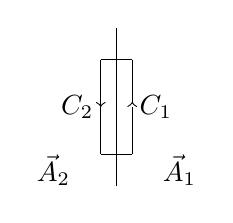
\begin{tikzpicture}[scale=0.2]
        \draw[-] (0,-5) -- (0,5);
        \draw[->] (-1,3)--(-1,0);
        \draw[-] (-1,-3)--(-1,0);
        \draw[-<] (1,3)--(1,0);
        \draw[-] (1,-3)--(1,0);
        \draw[-] (-1,3)--(1,3);
        \draw[-] (-1,-3)--(1,-3);
        \node at (-4, -4) {$\vec{A}_2$};
        \node at (4, -4) {$\vec{A}_1$};
        \node at (-2.5, 0) {$C_2$};
        \node at (2.5, 0) {$C_1$};
    \end{tikzpicture}
    \caption{Amperian Loop}
    \label{4.8.Loop}
\end{figure}
Then we can examine the curl. Constructing an Amperian loop as in \ref{4.8.Loop} normal to the surface of negligible thickness (usual protocol) we found for electrostatics
\begin{align}
    \oint\limits_C d\vec{l} \cdot \vec{E} &= \int\limits_{C_1}^{}\vec{E}_1 \cdot -d\vec{l} + \int\limits_{C_2}^{}\vec{E}_2 \cdot d\vec{l}\\
    0 &= 
\end{align}
because $\vec{\nabla}\vec{E} = 0$. Then in magnetostatics we obtain instead
\begin{align}
    \mu_0\int\limits_{C'}^{}dl \hat{t}\cdot \vec{\kappa} &= \int\limits_{C_1}^{}\vec{B}_1 \cdot (-d\vec{l}) + \int\limits_{C_2}^{}\vec{B}_2 \cdot d\vec{l}
\end{align}
with $\hat{t}$ the normal to the loop itself; note that this just reflects the fact that the current sourcing $\vec{B}$ along the loop must run normal to the loop. We then can change the bounds of integration to make everything over $C'$ (In the limit as the loop acquires zero height $C_1 = C_2$) and then equating integrands we obtain
\begin{align}
    \mu_0 \hat{t}\cdot \vec{\kappa} &= \hat{s}\cdot\left[ \vec{B}_2 - \vec{B}_1 \right]\\
    \vec{B}_2 - \vec{B}_1 &= \mu_0\vec{\kappa}\times \hat{n}\\
    \hat{n}\times\left[\vec{B}_2 - \vec{B}_1\right] &= \mu_0\vec{\kappa}
\end{align}

We can then examine BCs on $\vec{A}$. It is easy to see under Coulomb gauge that $\vec{A}_2 - \vec{A}_1 = 0$. Moreover, since $\vec{B}$ is not singular enough ever (no delta functions) and $\vec{A}$ goes with the flux through any arbitrary loop about the interface, so tangential component must also be continuous as $\vec{A}_1 = \vec{A}_2$ in the absence of nonzero flux.

We can then look at BCs on the derivatives of $\vec{A}$, much more interesting. We begin with $\nabla^2 \vec{A} = \mu_0 \vec{J}$, which then dotting both sides with some arbitrary $\vec{x}$ yields
\begin{align}
    \nabla^2(\vec{x}\cdot\vec{A}) &= \mu_0(\vec{x}\cdot\vec{J})\\
    \vec{\nabla}\cdot\left[ \vec{\nabla}(\vec{x} \cdot \vec{A}) \right] &= \mu_0 \vec{x}\cdot \vec{J}
\end{align}
If we then examine only surface components, i.e. $\vec{\nabla} \to \hat{n}[\vec{A}_2 - \vec{A}_1]$ then we obtain (removing $\vec{x}$)
\begin{align}
    \hat{n}\cdot\vec{\nabla}\left[ \vec{A}_2 - \vec{A}_1\right] &= \mu_0 \vec{\kappa}
\end{align}

If we then examine $\vec{\nabla}\times \vec{\nabla}\vec{A} = 0$, then we can decompose $\vec{A}$ into its tangential component which must also satisfy the equation ($\vec{A} = \hat{x} \cdot \vec{A} + \hat{y}\cdot \vec{A} \dots$ each of which individually satisfy the above equation) and we see
\begin{align}
    \hat{s}\cdot \vec{\nabla}\left[ \vec{A}_2 - \vec{A}_1 \right] &= 0
\end{align}

Let's then look at the multipole expansion. Consider a small localized current distribution, so $r_< = r', r_> = r$. Then
\begin{align}
    \vec{A} &= \frac{\mu_0}{4\pi}\int\limits_{V}^{}d\tau\;\frac{\vec{J}(\pvec{r})}{\abs{\vec{r} - \pvec{r}}}\\
    \frac{1}{\abs{\vec{r} - \pvec{r}}} &= \sum_{l=0}^{\infty}\frac{r_<^l}{r_>^{l+1}}P_l(\underbrace{\cos (\hat{r} \cdot \hat{r}')}_{\gamma})\\
    \vec{A}(\vec{r)} &= \frac{\mu_0}{4\pi r}\sum_{l=0}^{\infty}\frac{1}{r^l}\int\limits_{V}^{}d\tau\;\vec{J}(\pvec{r})(r')^lP_l(\cos\gamma)
\end{align}

This will inevitably end up being pretty messy, but just to have a taste of this we will examine what happens in the $l=0$ term; we expect it to vanish b/c no monopoles. So
\begin{align}
    \vec{A}_0(\vec{r}) = \frac{\mu_0}{4\pi r}\int\limits_{V}^{}\vec{J}\;d\tau
\end{align}

Now we will use $\vec{\nabla}\cdot (f\vec{a}) = f\vec{\nabla}\cdot \vec{a} + \vec{a} \cdot \vec{\nabla}f$ for $\vec{a} = \vec{J}, f = r_i = \vec{r} \cdot \hat{r}_i$. This then gives
\begin{align}
    \vec{\nabla}\cdot(r_i\vec{J}) &= r_i\vec{\nabla}\cdot\vec{J} + \vec{J} \cdot \vec{\nabla}r_i
\end{align}

The first term vanishes under steady state currents, so
\begin{align}
    \vec{\nabla}\cdot (r_i\vec{J}) &= \sum_{j=1}^{3}J_j \pd{}{r_j}r_i = \sum_{j=1}^{3} J_j \delta_{ij}\\
    &= J_i\\
    \int\limits_{V}^{}J_i(\pvec{r})d\tau' &= \int\limits_{V}^{}d\tau'\;\vec{\nabla}\cdot(r_i' \vec{J}(\pvec{r}))\\
    &= \oint\limits_S d\vec{S}\cdot \left( r_i'\vec{J}(\pvec{r}) \right)\\
    &= 0
\end{align}
because $\vec{J}$ is localized. Then since all three components vanish the entire $\vec{A}_0$ must also vanish.

We can then look at the dipole term
\begin{align}
    \vec{A}_2(\vec{r}) &= \frac{\mu_0}{4\pi r^2}\int\limits_{V}^{}d\tau'\;\vec{J(\pvec{r})}r' P_1(\cos\gamma) \\
    &= \frac{\mu_0}{4\pi r^3}\int\limits_{V}^{}d\tau'\;\vec{J}(\pvec{r}) \vec{r}\cdot \pvec{r}
\end{align}

From here forward it is very messy (check lecture notes) but we will go to index notation and use $\vec{\nabla}\cdot (r_ir_i\vec{J}) = r_jJ_i + r_iJ_j$ and adopt Levi-Civita notation for cross products $\vec{a}\times \vec{b} = \epsilon_{emn}a_mb_n$. Then applying an identity $\epsilon_{kij}\epsilon_{kmn} = \delta_{im}\delta_{jn} - \delta_{jm}\delta_{in}$ (resulting from taking two curls) we can simplify everything out and obtain
\begin{align}
    \vec{A}_1(\vec{r}) &= -\frac{\mu_0}{4\pi r^3} \frac{1}{2}\vec{r}\times \int\limits_{V}^{}d\tau\;\left[ \pvec{r}\times \vec{J}(\pvec{r}) \right]
\end{align}

Then if we define $\vec{M}(\vec{r}) = \frac{1}{2}\vec{r}\times\vec{J}(\vec{r})$ and $\vec{m} = \int\limits_{V}^{}d\tau'\;\vec{M}(\pvec{r})$ we can rewrite
\begin{align}
    \vec{A}_1(\vec{r}) &= \frac{\mu_0}{4\pi}\frac{\vec{m}\times \vec{r}}{r^3}
\end{align}

Note that this looks very similar to the dipole potential! Note that while the vector algebra omitted is brutal, you will be responsible for knowing it! 

We can then look at a current loop, for which $I$ is constant below
\begin{align}
    \vec{A}_1(\vec{r}) &= -\frac{\mu_0}{4\pi r^3}\frac{1}{2}\vec{r}\times \oint\limits_C \pvec{r}\times Id\vec{l}\\
    &= -\frac{\mu_0}{4\pi}\frac{I}{r^3}\vec{r}\times \oint\limits_C \frac{\pvec{r} \times d\vec{l}}{2}
\end{align}

Then upon examination we find that $\frac{\vec{r}\times d\vec{l}}{2}$ is just the area of an infinitisemal slice of the loop, so we obtain
\begin{align}
    \vec{A}_1 &= -\frac{\mu_0}{4\pi}\frac{I}{r^3} \vec{m}_{loop} \times \vec{r}\\
    \vec{m}_{loop} &= I\oint\limits_C \frac{\pvec{r} \times d\vec{l}}{2}\\
    &= I\vec{a}
\end{align}
with $\vec{a}$ the area vector of the loop (note orientation! Correct right hand rules with $\vec{I}$). This produces field (again, in notes)
\begin{equation}
    \vec{B} = \vec{\nabla}\times \vec{A} = \frac{\mu_0}{4\pi}\frac{3(\vec{m}\cdot \hat{r}) \hat{r} - \vec{m}}{r^3}
\end{equation}

We can then look at forces on a mangetic dipole. We begin with expression
\begin{align}
    \vec{F} &= \int\limits_{V}^{}d\tau'\;\vec{J}(\vec{r}) \times \vec{B}(\vec{r})
\end{align}

Then approximating that the dipole itself is small, we will approximate $B_k(\vec{r}) = B_k(\vec{0}) + \pd{B_k}{r_m}\Big|_{\vec{0}}r_m$ with $\vec{0}$ the center of the distribution. Then
\begin{align}
    \vec{F} &= \sum_{ijk}^{}\epsilon_{ijk} \hat{r}_i\left[ B_k(\vec{0})\int\limits_{V}^{}d\tau'\;\vec{J}(\pvec{r}) + \pd{B_k}{r_m}\Big|_{\vec{0}}\int\limits_{V}^{}d\tau'\;J_kr_m \right]\\
    &= \vec{\nabla}(\vec{m}\cdot \vec{B}) - \vec{m}\left( \vec{\nabla}\cdot \vec{B} \right)\Big|_{\vec{0}}\\
    &= \vec{\nabla}\left( \vec{m}\cdot \vec{B} \right)
\end{align}
due to vanishing $\vec{\nabla}\cdot \vec{B}$.

We can also compute torque! We only care again about the first order term which yields
\begin{align}
    \vec{N} &= \int\limits_{V}^{}d\tau'\;\vec{r}\times\left[ \vec{J}\times\vec{B} \right]\\
    &\;\;\;\vdots\\
    &= \vec{m} \times \vec{B}(\vec{0})
\end{align}

See notes for algebra!

\chapter{4/10/14 --- Magnetostatics in matter}

We first should look at forces, torques, and energy of magnetic dipoles. First we know that the force is given
\begin{equation}
    \vec{F} = \vec{\nabla}(\vec{m}\cdot \vec{B})
\end{equation}
torque
\begin{equation}
    \vec{N} = \vec{m}\times \vec{B}
\end{equation}
and energy
\begin{equation}
    U = -\vec{m}\cdot \vec{B}
\end{equation}

Note that the dipole seeks out areas of stronger field. This should be bothersome,, because the magnetic field seems like it can do work now! The classical explanation is that the current driving the field does the work, either by losing energy or drawing power from some external battery. The quantum mechanical explanation actually yields a violation, because you can actually do work on the intrinsic spin! The electron (e.g.) spin doesn't arise from a current; the reason that this occurs is because the spin doesn't arise from a current but is a fundamental property and so doesn't obey the Lorentz force law from which we derived the fact that $\vec{B}$ does no work.

Then we look at magnetic materials. Define \emph{dimagnetic} to be analogous to dielectrics, so that $\vec{m} \propto -\vec{B}$ pointing in the opposite direction. This arises as an interaction of the field with magnetic dipoles in the material.

There are two other kinds, \emph{paramagnetic} and \emph{ferromagnetic} materials, which respond due to interactions with unpaired electrons. (Note: unpaired electrons are favored because they have overlapping spatial wavefunctions, so Coulomb repulsion!). Both odd-numbered electrons and exchange interaction (unpaired electrons) exhibit a net $\vec{m}$ due to the spins. Thus para/ferromagnetic comes from interactions with the spin. Thus, paramagnetism is nonlinear in general; we will return to this. Ferromagnetic systems exhibit crystal lattice effects that remain polarized as the driving field is taken away.

We will begin by talking about bound currents in magnetized objects. Given some $d\vec{m} = \vec{M}(\vec{r}) d\tau$ magnetization density $\vec{M}$ (macroscopic), analogous to $\vec{P}$. Then this magnetic dipole produces potential contribution
\begin{align}
    d\vec{A} &= \frac{\mu_0}{4\pi}\frac{d\vec{m} \times (\vec{r} - \pvec{r})}{\abs{\vec{r} - \pvec{r}}^3}\\
    \vec{A} &= \int\limits_{V}^{}d\vec{A}\;d\tau\\
    &= \frac{\mu_0}{4\pi}\int\limits_{V}^{}d\tau'\;\vec{M}(\pvec{r}) \times \vec{\nabla}_{r'}\left( \frac{1}{\vec{r} - \pvec{r}} \right)\\
    &= \frac{\mu_0}{4\pi}\int\limits_{V}^{}d\tau\;\frac{\vec{\nabla}_{r'}\times \vec{M}}{\abs{\vec{r} - \pvec{r}}} - \frac{\mu_0}{4\pi}\int\limits_{V}^{}d\tau\;\vec{\nabla}_{r'}\left( \frac{\vec{M}}{\abs{\vec{r} - \pvec{r}}} \right)
\end{align}
where we use $\vec{\nabla} \times (f\vec{a}) = f\vec{\nabla}\times \vec{a} - \vec{a}\cdot \vec{\nabla}f$. We can then use vector identity (Stokes Theorem?) to convert this expression to
\begin{align}
    \vec{A} &= \frac{\mu_0}{4\pi}\left[ \int\limits_{V}^{}d\tau\;\frac{\vec{\nabla}\times \vec{M}}{\abs{\vec{r} - \pvec{r}}} + \int\limits_{S}^{}\frac{\vec{M}\times d\vec{S}}{\abs{\vec{r} - \pvec{r}}}\; \right]
\end{align}

We can then identify $\vec{J}_b = \vec{\nabla} \times \vec{M}$ and $\vec{K}_b = \vec{M}\times \hat{n}$ bound volume and surface current densities respectively.

Let's now look at a sphere that is uniformly magnetized. Let's magnetize the sphere in the $\hat{z}$ direction with $\vec{M}$ and place the sphere at the origin. We then note that $\vec{J}_b = \vec{\nabla}\times \vec{M}= 0$ because $\vec{M}$ is uniform. Then $\vec{K}_b = \vec{M} \times \hat{n} = M\sin\theta \hat{ \phi}$. Then we can compute
\begin{align}
    \vec{A} &= \frac{\mu_0}{4\pi}R^2 \int\limits_{0}^{2\pi}d\phi'\int\limits_{0}^{\pi}d\theta'\;\sin\theta' \frac{M\sin\theta' \hat{\phi}}{\abs{\vec{r} - \pvec{r}}}\\
    &= \frac{\mu_0}{4\pi}R^2 \int\limits_{0}^{2\pi}d\phi'\int\limits_{0}^{\pi}d\theta\;\frac{M\sin^2\theta'\left( -\hat{x}\sin \phi' + \hat{y}\cos \phi' \right)}{\abs{\vec{r} - \pvec{r}}}
\end{align}
It turns out that using the spherical harmonic expansion of $\frac{1}{\abs{\vec{r} - \pvec{r}}}$ and noting $\sin\theta'(-\hat{x}\sin\phi' + \hat{y}\cos\phi') \sim Y_{1m}$ a sum of a few spherical harmonics. Thus a few coefficients get pulled out and we can arrive at
\begin{align}
    \vec{A} &= \frac{\mu_0}{4\pi}R^2M\frac{4\pi}{3}\frac{r_<}{r_>^2}\sin\theta\left( -\hat{x}\sin\phi + \hat{y}\cos\theta \right)\\
    &= \begin{cases}
        \frac{\mu_0}{3}Mr\sin\theta\hat{\phi} & r \leq R\\[10pt]
        \frac{\mu_0}{3}\frac{R^3}{r^2}M\sin\theta\hat{\phi} & r \geq R\\
    \end{cases}
\end{align}

Note that we have to use the full spherical harmonic expansion rather than the Legendre polynomials because the integral for arbitrary $\vec{r}$ isn't azimuthally symmetric. It then is evident upon inspection that outside the sphere the field looks like a dipole for $\vec{m} = \left( \frac{4\pi}{3}R^3M \right)\hat{z}$, or just $\vec{M}V$ with $V$ the volume! 

Let's then look at the $\vec{B}$ field, which is $\frac{2}{3}\mu_0\vec{M}$ inside the sphere (constant) and dipole outside! Let's note differences between the two, electrostatic vs magnetostatic respectively
\begin{align}
    r & \leq R & \vec{E} &= -\frac{1}{3\epsilon_0}\vec{P} & \vec{B} &= \frac{2}{3}\mu_0 \vec{M}\\
    r & \geq R & V &= \frac{1}{4\pi\epsilon_0} \frac{\vec{p}\cdot \hat{r}}{r^2} & \vec{A} &= \frac{\mu_0}{4\pi}\frac{\vec{m}\times \hat{r}}{r^2}
\end{align}

We can then look at the auxiliary field. Examining $\frac{1}{\mu_0}\vec{\nabla}\times \vec{B} = \vec{J}_f + \vec{\nabla}\times \vec{M}$ the $\vec{J}_b$ then we can define $\vec{H} = \frac{\vec{B}}{\mu_0} - \vec{M}$ such that $\vec{\nabla}\times \vec{H} = \vec{J}_f$. Then the integral form of Ampere's Law is also true for $\vec{H}, \vec{J}_f$. 

We must also look at the divergence $\vec{\nabla}\cdot \vec{H} = -\vec{\nabla}\cdot \vec{M}$ so any time there is a divergence in $\vec{M}$ we have to be more careful. Then we can calculate our $\vec{M}$ on uniformly magnetized sphere
\begin{equation}
    \vec{H}(r \leq R) = -\frac{1}{3}\vec{M}
\end{equation}
and outside it is just $\vec{B}/\mu_0$. This is why $\vec{\nabla}\cdot \vec{H}$ is important, because there is no $\vec{J}$ and so if $\vec{H}$ has both vanishing curl and div then it's boring (\dots but $\vec{\nabla} \cdot \vec{M} = 0$ right?).

Note that we control $V, \vec{J}_f$ in actual experiments, which means we use $\vec{E}, \vec{H}$ a lot more than we use $\vec{D}, \vec{B}$ respectively.

Let's now look at BCs on $\vec{H}$. We recall that $\vec{\nabla} \cdot \vec{B} = 0$ shows that $\hat{n}\cdot \vec{B}$ was continuous, so
\begin{equation}
    \hat{n}\cdot \left[ \vec{H}_2 - \vec{H}_1 \right] = -\hat{n}\cdot \left[ \vec{M}_2 - \vec{M}_1 \right]
\end{equation}

Also by a loop argument we can find
\begin{align}
    \left[ \vec{H}_2 - \vec{H}_1 \right]\cdot\hat{s} &= [\vec{K}_f \times\hat{n}]\cdot \hat{s}\\
    \hat{t}\cdot\left( \hat{n}\cdot \left[ \vec{H}_2 - \vec{H}_1 \right] \right) &= \hat{t}\cdot \vec{K}_f\\
    \hat{n} \times \left[ \vec{H}_2 - \vec{H}_1 \right] &= \vec{K}_f
\end{align}

Linear materials have $\vec{M} = \chi_m \vec{H}$ with $\chi_m$ the magnetic susceptibility, and then if we define $\vec{B} = \mu_0\left( \vec{H} + \vec{M} \right) = \mu \vec{H}, \mu = \mu_0(1 + \chi_m)$. Note that $\chi_m > 0$ for paramagnets, $\chi_m < 0$ for dimagnets.

Example, magnetic rod with uniform current density and $\chi_m, \mu$, then $J = \frac{I}{\pi R^2}$ then we apply Ampere's Law under the stipulation of rotationally symmetric and field only in $\hat{\phi}$ direction to obtain
\begin{equation}
    \vec{H} =
    \begin{cases}
        \frac{I}{2\pi s}\frac{s^2}{R^2}\hat{\phi} & s \leq R\\[10pt]
        \frac{I}{2\pi s}\hat{\phi} & s \geq R
    \end{cases}
\end{equation}

We now go about finding everything else in detail. First, for $s > R$ we have $\vec{M} = 0, \vec{B} = \mu_0 \frac{I}{2\pi s}\hat{\phi}$. Inside we have 
\begin{align}
    \vec{M} = \chi_m\vec{H} &= \frac{\mu - \mu_0}{\mu}\frac{I}{2\pi s}\frac{s^2}{R^2}\hat{\phi}\\
    \vec{B} = \mu \vec{H} &= \mu \frac{I}{2\pi s}\frac{s^2}{r^2}\hat{\phi}
\end{align}

Let's then check BCs. We don't need to worry about the BCs in the $\hat{z}$ direction or the radial direction because zero magnitude field, so we just look at 
\begin{align}
    \hat{\phi}\cdot \vec{H}(s=R) = \frac{I}{2\pi R}
\end{align}
is indeed continuous, and so we can note also that $\hat{\phi}\cdot \frac{\vec{B}}{\mu}, \hat{\phi}\cdot \frac{\vec{M}}{\chi_m}$ are both continuous across the boundary.

Let's then compute bound currents
\begin{align}
    \vec{K}_b &= \vec{M}\times\hat{n} = -\chi_m \frac{I}{2\pi R}\hat{z}\\
    \vec{J}_b &= \chi_m \vec{J}_f
\end{align}

\chapter{4/15/14 --- Magnetostatic BVPs}

There are a few types of nonlinear magnetism:
\begin{itemize}
    \item paramagnetism
    \item ferromagnetism - electrons in various spin states interact with neighboring spins in the crystal lattice, creating ``domains'' inside the lattice that align only when strong field is applied, hysteresis means the magnet ``remembers'' previous configurations.
    \item exchange interaction - coulomb repulsion; $\psi_1\ket{\uparrow} + \psi_1\ket{\downarrow}$ is less preferred than $\psi_1\ket{\uparrow} + \psi_2\ket{\uparrow}$
\end{itemize}

We will now discuss BVPs in magnetostatics (not in Griffiths, Jackson 5.9-12). We know that $\vec{B} = \vec{\nabla}\times \vec{A}, \vec{\nabla}\times \vec{H} = \vec{J}_f$. So then since $\vec{H}$ is a function of $\vec{B}$ we could write $\vec{\nabla} \times \vec{H}(\vec{\nabla}\times \vec{A}) = \vec{J}_f$, but it is difficult in general to solve this. We can simplify under the assumption of linear, homogeneous and end up with
\begin{align}
    \vec{\nabla} \times \left( \frac{1}{\mu}\vec{\nabla}\times \vec{A} \right) &= \vec{J}_f\\
    \vec{\nabla} \times (\vec{\nabla} \times \vec{A}) &= \mu \vec{J}_f\\
    \nabla^2 \vec{A} = -\mu \vec{J}_f
\end{align}
which almost looks like a Poisson Equation term by term subject to boundary conditions $\hat{n} \times \vec{B}$ or $\vec{A}$ BCs on boundaries.

Then if there are no free currents we can write a magnetostatic scalar potential, as $\vec{\nabla}\times \vec{H} = 0$ which means $\vec{H} = -\vec{\nabla}V_M$. This then leads naturally to $\nabla^2 V_m = 0$ when $\vec{\nabla}\cdot(\mu (-\vec{\nabla}V_m)) = 0$.

There is another regime that we can work under, called the hard ferromagnetic regime, under which $\vec{M}$ is fixed and no free currents. Under this case, $\vec{B} = \mu_0(\vec{H} + \vec{M})$ (note that $\vec{B} \neq \mu\vec{H}$ because we are not working with linear material!), and if we apply $\vec{\nabla}\cdot$ on both sides we find ($\vec{\nabla}\cdot \vec{B} = 0, \vec{\nabla} \cdot \vec{H} = -\vec{\nabla}V_m$)
\begin{equation}
    \nabla^2 V_m = -\vec{\nabla}\cdot \vec{M}
\end{equation}
so it is a Poisson's equation sourced by $\vec{\nabla}\cdot \vec{M}$. Then with a sufficiently simple boundary condition we can solve this; recall the general solution then looks like $V_m(\vec{r}) = -\frac{1}{4\pi}\int\limits_{}^{}d\tau'\;\frac{\vec{\nabla}\cdot \vec{M}}{\abs{\vec{r} - \pvec{r}}}$. If the BCs are not simple, we can use the analogy to electrostatics to write
\begin{equation}
    V_m(\vec{r}) = -\frac{1}{4\pi}\int\limits_{V}^{}d\tau'\;\frac{\vec{\nabla}\cdot\vec{M}}{\abs{\vec{r} - \pvec{r}}} + \frac{1}{4\pi}\int\limits_{S}^{}da'\;\frac{\hat{n}\cdot\vec{M}}{\abs{\vec{r} - \pvec{r}}}
\end{equation}
so it's the result of bound volume charge $-\vec{\nabla}\cdot \vec{M}$ and bound surface charge $\hat{n}\cdot\vec{M}$.

Let's do an example now, same uniformly magnetized sphere, so given $\vec{M}$ not influence by any free current. Then $\vec{M}$ is uniform so $\rho_M = -\vec{\nabla}\cdot \vec{M} = 0$ and $\sigma_m = \hat{n}\cdot \vec{M} = M\cos\theta$. This then looks exactly like a uniformly polarized sphere! So we just replace $\vec{P} \to \vec{M}$ is the solution that we've already computed, and we obtain
\begin{align}
    V_m(r \leq R) &= \frac{Mz}{3} & V_m(r \geq R) &= \frac{m \cdot \hat{r}}{4\pi r^3}
\end{align}
with $m = \frac{4}{3}\pi R^3 \vec{M}$. This then looks like a perfect dipole outside.

Note that if we want $\vec{B}$ we \textbf{CANNOT} just use $\vec{B} = \mu \vec{H}$ because we are not in a linear material; instead we must do $\vec{B} = \mu_0(\vec{H} + \vec{M})$. This then gives $\vec{B}(r \leq R) = \frac{2}{3}\mu_0\vec{M}$ and $\mu_0\vec{H}$ outside since $\vec{M}$ vanishes outside.

Note that in the electrostatic case induced dipoles pointed \emph{against} $\vec{E}$ while in the magnetostatic case induced dipoles point \emph{with} $\vec{B}$ (though $\vec{H}$ is opposite to $\vec{M}$). 

Note we can also calculate the case for hard ferromagnetism using the vector potential, under which $\vec{M}$ is fixed and $\vec{J}_f = 0$, then we can compute bound currents and solve.

Let's look at a magnetically permeable sphere in external field, with an electric field $\vec{B}_0, \vec{M}_0$ pointing in the $\hat{z}$ direction and sphere with $\mu$. We note this is identical to the electric case, and the correspondence looks as below
\begin{align}
    \rho_b &= -\vec{\nabla}\cdot\vec{P} & \rho_m &= -\vec{\nabla}\cdot \vec{M}\\
    \sigma_b &= \hat{n}\cdot \vec{P} & \sigma_M &= \hat{n} \vec{M}\\
    \epsilon_0 \vec{E} &= -\epsilon_0 \vec{\nabla}V & \vec{H} &= -\vec{\nabla}V_M\\ 
    \epsilon_0\nabla^2V &= -\rho_b & \nabla^2 V_M &= -\rho_M\\
    \vec{D} &= \epsilon_0\vec{E} + \vec{P} & \frac{\vec{B}}{\mu_0} &= \vec{H} + \vec{M}
\end{align}

We must also check for boundary conditions being identical
\begin{align}
    \hat{n} \cdot \left[ \epsilon_0 \vec{E}_>(R) - \epsilon_0\vec{E}_<(R) \right] &= \sigma_b & \hat{s} \cdot \left[ \epsilon_0 \vec{E}_>(R) - \epsilon_0\vec{E}_<(R) \right] &= 0\\
    \hat{n}\cdot \left[ \vec{H}_>(R) - \vec{H}_<(\vec{R}) \right] &= \hat{n}\left[ \vec{M}_>(R) - \vec{M}_<(R) \right] & \hat{s} \cdot \left[ \vec{H}_>(R) - \vec{H}_<(R) \right] &= 0\\
    &= \hat{n}\cdot\vec{M}_<(R) = \sigma_M
\end{align}
as $\vec{M}_>(R) = 0$ and the tangential BC holds because no $\vec{J}_f, \vec{\kappa}_f$. Then we have the correct correspondence and we can just use the old solution. 

Let's do a more specific case, that will show magnetic shielding. We will compute with a magnetically permeable spherical shell and apply a uniform field $\vec{H}_0$ along the $z$ axis. We will do this with separation of variables. Since the potential does not have any source at the origin, the setup looks like
\begin{align}
    V_1(r < a) &= \sum_{l}^{}A_lr^lP_l(\cos\theta)\\
    V_2(a < r < b) &= \sum_{l}^{}\left( C_lr^l + \frac{D_l}{r^{l+1}} \right)P_l(\cos\theta)\\
    V_3(r > b) &= -H_0r\cos\theta + \sum_{l}^{}\frac{E_l}{r^{l+1}}P_l(\cos\theta)
\end{align}

Instead of going through the $\vec{D}$ field as we would in electrostatics, we will instead start by requiring continuity of components of $\vec{B}$ (specifically, tangential conditions replacing conditions on $D$). This then looks for the normal components
\begin{align}
    \mu_0 \pd{V_1}{r} &= \mu \pd{V_2}{r} & \mu\pd{V_2}{r} &= \mu_0\pd{V_3}{r}
\end{align}
and tangential component
\begin{align}
    \pd{V_1}{\theta} &= \pd{V_2}{\theta} & \pd{V_2}{\theta} &= \pd{V_3}{\theta}
\end{align}

We note that this is the only tangential component that we are concerned with, because of azimuthal symmetry. At this point, we must note that derivatives of Legendre Polynomials produce Associated Legendre Polynomials, as
\begin{align}
    P_l^m(x) &= \left( -1 \right)^m(1-x^2)^{m/2}\left( \rd{}{x} \right)^mP_l(x)\\
    \rd{}{\theta}P_l(\cos\theta) &= (-\sin\theta)\rd{}{\cos\theta}P_l(\cos\theta)\\
    &= \frac{P_l^1(\cos\theta)}{(-1)(1-\cos^2)^{1/2}}(-\sin\theta) = P_l^1(\cos\theta)
\end{align}

Then noting that $P_l^1$ are orthonormal on $\theta$ we can just equate coefficients like we did before. We then can see that the matching conditions are
\begin{align}
    \mu_0lA_la^{l-1} &= \mu lC_la^{l-1} - \mu(l+1)\frac{D_l}{a^{l+2}}\\
    \mu l C_l b^{l-1} - \mu(l+1)\frac{D_l}{b^{l+2}} &= -\mu_0 H_0 \delta_{l1} - \mu_0 (l+1)\frac{E_l}{b^{l+1}}\\
    A_l a^l &= C_la^l + \frac{D_l}{a^{l+1}}\\
    C_lb^l + \frac{D_l}{b^{l+1}} &= -H_0b\delta_{l1} + \frac{E_l}{b^{l+1}}
\end{align}
coming from matching $\rd{V}{r}$ at $r=a,b$ and $\rd{V}{\theta}$ at $r=a,b$ respectively. This will ultimately produce magnetic fields (which are much more intuitive than potentials):
\begin{align}
    \vec{H}_1 &= -\frac{q}{2}\frac{H_0\hat{z}}{\alpha}\\
    \vec{H}_2 &= \frac{3H_0\hat{z}}{\alpha} + \frac{3(\vec{m}_a\cdot \hat{r})\hat{r} - \vec{m}_a}{4\pi r^3}\\
    \vec{H}_3 &= H_0\hat{z} + \frac{3(\vec{m}_b\cdot \hat{r})\hat{r} - \vec{m}_b}{4\pi r^3}\\
    \alpha &= \frac{\mu}{\mu_0}\left( 1 - \frac{a^3}{b^3} \right)\\
    \vec{m}_a &= -\frac{q}{2}\frac{H_0}{\alpha}(\frac{4}{3}\pi a^3)\hat{z}\\
    \vec{m}_b &= 3\left[ 1 - \frac{3}{\alpha} \right]H_0\left(\frac{4 \pi b^3}{3}\right)\hat{z}
\end{align}
\chapter{4/17/14 --- Starting Electrodynamics}

Let's finish up the shell that we talked about last lecture. Recall that our final result for the field under $\mu \gg \mu_0$ was
\begin{align}
    \vec{H}_1 &= -\frac{q}{2}\frac{H_0\hat{z}}{\alpha}\\
    \vec{H}_2 &= \frac{3H_0\hat{z}}{\alpha} + \frac{3(\vec{m}_a\cdot\hat{r})\hat{r} - \vec{m}_a}{4\pi r^3}\\
    \vec{H}_3 &= H_0\hat{z} + \frac{3(\vec{m}_b \cdot \hat{r})\hat{r} - \vec{m}_b}{4\pi r^3}
\end{align}
for $\alpha = \frac{\mu}{\mu_0}\left( 1 - \frac{a^3}{b^3} \right)$. This looks like a bunch of field lines that get squished into the shell and evade the cavity in the middle. Note that this looks different from the conducting shell from electrostatics!

Let's then try to solve this by surface currents. Recall that $\vec{\kappa} = \frac{1}{\mu_0}\hat{n}\times \Delta \vec{B}$. We can rewrite this
\begin{align}
    \vec{\kappa} &= \frac{1}{\mu_0}\hat{n}\times \Delta \vec{B}\\
    &= \frac{1}{\mu_0} \left[ -\frac{\mu_<}{r}\pd{V_<}{\theta} + \frac{\mu_>}{r}\pd{V_>}{\theta} \right]\\
    &= \frac{\mu_< - \mu_>}{\mu_0}\frac{1}{r}\pd{V_M}{\theta}\\
    &= \frac{\mu_< - \mu_>}{\mu_0} H_\theta
\end{align}

Recall then our permanently magnetized sphere has
\begin{equation}
    \vec{B}_M =
    \begin{cases}
        \frac{2}{3}\mu_0\frac{\vec{\kappa}\cdot \hat{\phi}}{\sin\theta}\hat{z} & r \leq R\\
        \frac{\mu_0}{4\pi}\frac{3(\vec{m} \cdot \hat{r}) - \vec{m}}{r^3}
    \end{cases}
\end{equation}
with $\vec{m} = \frac{4}{3}\pi R^3\frac{\vec{\kappa}\cdot \vec{\phi}}{\sin\theta}\hat{z}$.

Now since we know $\vec{\kappa}$ for our current configuration, we can take superpositions of the two spheres (looks like $\cos\theta$) and obtain
\begin{align}
    \vec{B}_1(r,\theta) &= \vec{B}_0 + \frac{2}{3}\mu_0\frac{\vec{\kappa}_a(a)\cdot\hat{\phi} + \vec{\kappa}_b(b)\cdot\hat{\phi}}{\sin\theta}\label{4.17.B1}\\
    \vec{B}_2(r,\theta) &= \vec{B}_0 + \frac{2}{3}\mu_0 \frac{\vec{\kappa}_b(b)\cdot\hat{\phi}}{\sin\theta} + \frac{\mu_0}{4\pi}\frac{3(\vec{m}_a\cdot\hat{r})\hat{r - \vec{m}_a}}{r^3}
\end{align}
and similarly for $\vec{B}_3$.

Then we know that the inside should be shielded by a factor of $\mu_0/\mu$ so we know that the second term in \eqref{4.17.B1} must cancel the first term and recontribute a $\mu_0/\mu$ order. Let's look then at this second term without bashing the algebra at first
\begin{align}
    \mu_0\kappa &= \mu_0\left( \frac{\mu - \mu_0}{\mu_0} \right)\frac{1}{r}\pd{V_M}{\theta}\\
    &= \left( \frac{\mu}{\mu_0} - 1 \right)\mu_0H_0
\end{align}
which has the requisite piece to cancel the first piece, as $\mu_0H_0 = B_0$. But then since we realize that we've left out a term with a $\frac{\mu_0}{\mu}$ order, we can never obtain an exact result through surface currents up to $\frac{\mu_0}{\mu}$ order (I have no idea where that term came from which is why I'm not going to write it down\dots looks like it comes in front of the $H_0$ above; it arises because we don't use the exact $H_1$ so there are corrective terms in $\kappa$, so circular!). This means we cannot ever compute the residual field post-shielding.

However, we can certainly get up to $\frac{\mu}{\mu_0}$ to zeroth order easily; he's going to bash this but I don't plan to. Just compute $H_1$ up to zeroth order in $\frac{\mu}{\mu_0}$. This confirms that the zeroth order field is shielded and any residual field must be of order $\frac{\mu_0}{\mu}$.

We now start electrodynamics! There's a section on currents/Ohm's Law in Griffiths, so we just cite the results here. Note that $\vec{J} = \sigma \vec{E}$ with $\sigma$ computed by very simple model to be $\frac{nq^2\lambda}{2mv_{thermal}}$ (we won't use this formula). This proportionality is Ohm's Law. We can also compute the power $P = \vec{J}\cdot \vec{E}$. Integrating these two expressions over paths is what gives us $I = \frac{V}{R}$ wth $R = \frac{1}{\sigma}\frac{L}{A}$ and $P = \frac{V^2}{R} = I^2 R$. We will mostly stick with the differential forms for now.

We will examine under uniform $\sigma$ and steady states, which gives $\vec{\nabla}\cdot \vec{E} = \frac{1}{s}\vec{\nabla}\cdot \vec{J} = \pd{\rho}{t} = 0$. Note this shows $\rho$ is constant, and we will work with $\rho = 0$ in uniform conductors, or that Laplace's euation is satisfied. Then if we have, say, a wire carrying current, we can actually solve a BVP. 

In this specific case, the BCs are then notably that $\vec{J} \cdot \hat{n} = \vec{E}\cdot \hat{n} = 0$ along the sides of the wire, and at the ends we can fix the potential. These are then mixed BCs, Neumann and Dirichlet respectively, and we note that solution $V = \frac{\Delta V}{L}z, \vec{E} = \frac{\Delta V}{L}$ satisfies the BCs. This shows that $\vec{E}$ is uniform in a uniform conductor with constant dimensions.

Let's now look at electromotive forces. Suppose we move a wire of height $h$ at velocity $v$ and horizontal coordinate $x$ into a region with field $\vec{B}_0$. Wire is being pulled away from the magnetic field direction and has resistance $R$. So it is clear that charges in the wire feel $\vec{F} = -qvb\hat{y}$ (we pull wire in $\hat{x}$ direction). 
\begin{figure}[!h]
    \centering
    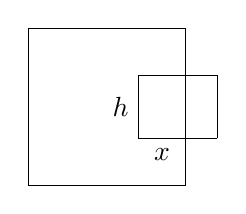
\begin{tikzpicture}[scale=0.2]
        \draw[-] (-5,-5) -- (-5,5);
        \draw[-] (-5,5) -- (5,5);
        \draw[-] (5,-5) -- (5,5);
        \draw[-] (5,-5) -- (-5,-5);
        \draw[-] (2,-2) -- (2,2);
        \draw[-] (2,2) -- (7,2);
        \draw[-] (7,-2) -- (7,2);
        \draw[-] (7,-2) -- (2,-2);
        \node[left] at (2,0) {$h$};
        \node[below] at (3.5,-2) {$x$};
    \end{tikzpicture}
    \caption{Wire setup; $\hat{x}$ points to right, $\hat{y}$ points up, wire pulled to right}
    \label{4.17.setup}
\end{figure}

Then we can see the work done by the field by integrating over the edge, so $W = qvBh$. However, $\vec{B}$ fields don't do work! The reason that this can happen is because it takes work to continue to pull the wire. This is because the moving charges in the $\hat{y}$ direction now exhibit a force in the $-\hat{x}$ direction, or $\vec{F} = -quB\hat{x}$ with $u$ velocity in the $x$ direction. Then the power of this work goes $quBv$, and the total amount of work done over as a particle moves along the vertical segment must be $P \frac{h}{u} = qBvh$ with $h/u$ the time elased, and so we find the works cancel. 

We can then write a relationship between the changing magnetic flux of the wire and the resulting $\varepsilon$ EMF. First,
\begin{equation}
    \Phi = \int\limits_{S}^{}d\vec{S} \cdot \vec{B}(\vec{r})
\end{equation}
and so
\begin{equation}
    \rd{\Phi}{t} = -\varepsilon
\end{equation}

Surprise! Let's do this the rigorous/generic way (the ``Ph106'' way instead of the ``Ph1'' way, oh dear). Take an arbitrary loop $C$ and have a translation $C(t + dt)$ in some magnetic field $\vec{B}$. Let's then compute the change in flux as the loop moves
\begin{align}
    d\Phi &= \int\limits_{S(t)}^{}d\vec{S}\cdot B - \int\limits_{S(t + dt)}^{}d\vec{S} \cdot \vec{B}
\end{align}

Then let's consider some volume $dV$ enclosed by the loop over this time $dt$ (i.e. with bases $S(t), S(t + dt)$ and height whatever). Then noting $\vec{\nabla}\cdot \vec{B} = 0$ we can compute this divergence as
\begin{align}
    \vec{\nabla}\cdot \vec{B} = 0 &= \int\limits_{S(t + dt)}^{}da \hat{n}_C \cdot \vec{B} - \int\limits_{S(t)}^{}da \hat{n}_C \cdot\vec{B} + \int\limits_{S'}^{}da \hat{n} \cdot \vec{B}
\end{align}
with $S'$ the surface on the side of the volume $dV$. Note that there is a sign flip because the normal $\hat{n}_C$ is opposite to the normal defined by the surface for one of the faces, since $\hat{n}_C$ can be defined to be the orientation defined by the contour (basically, the normal to the surfaces $S(t), S(t + dt)$ is in opposite directions but $\hat{n}_C$ is a single direction). Then since these give $d\Phi$ we find
\begin{align}
    d\Phi &= -\int\limits_{S'}^{}da \hat{n}\cdot \vec{B} = -\int\limits_{C(t)}^{}(d\vec{l} \times \vec{v}dt)\cdot \vec{B}
\end{align}
where we replace the area element with the cross product that gives its area. Then we of course only care about perpendicular velocity $\vec{v}_{\perp} = \vec{w}$, and then vector identity takes us to
\begin{align}
    d\Phi &= -\int\limits_{C(t)}^{}(d\vec{l} \times \vec{w}dt)\cdot \vec{B}\\
    &= -dt \int\limits_{C(t)}^{}d\vec{l} \cdot (\vec{w} \times \vec{B})\\
    \rd{\Phi}{t} &= -\int\limits_{C(t)}^{}d\vec{l} \cdot \frac{\vec{F}_m}{q} = -\varepsilon
\end{align}
where we recognize the Lorentz force. 

Let's do a quick example, AC current generator. Put a square (flat) loop of area $A$ in a magnetic field $\vec{B} \propto \hat{z}$ and spin it about the $\hat{y}$ direction, $\vec{\omega} \propto \hat{y}$. Then $\Phi(t) = AB_0\hat{z} \cdot \hat{n}(t) = AB_0\cos \omega t$. Thus $\varepsilon = -\rd{\Phi}{t} = AB\sin \omega t$. Next time we will talk about Faraday's Law.
\chapter{4/22/14 --- More Faraday's Law, Inductance}

Faraday's Law is the empirical observation that the same $\varepsilon$ appears when either a loop inside a field is moved and the field is held constant or the loop is held constant and the field changes in time. Recall that the form of Faraday's Law is
\begin{equation}
    \varepsilon = -\rd{\Phi}{t}
\end{equation}

Lenz's Law then says that $\varepsilon$ points in the direction to oppose the change in $\Phi$. We can understand Faraday's Law from a Galilean relativity perspective, where in the rest frame of the wire the field changes while in the lab frame the wire moves. It is also a consquencce of locality; the wire does not know whether the loop is moving or the field is changing.

Let's then examine the transformation of fields under Galilean relativity. Let $\pvec{F} = \oint d\vec{l} \cdot \pvec{E}$ be the force feld in the loop rest frame while $\vec{F}$ is in the field rest frame. Then
\begin{equation}
    \oint\limits_{C'} d\vec{l} \cdot \pvec{E} = \oint\limits_{C(t)} d\vec{l} \cdot \left[ \vec{E} + \vec{v} \times \vec{B} \right]
\end{equation}
which shows that $\pvec{E} = \vec{E} + \vec{v} \times \vec{B}$ which shows that the fields mix even without special relativity. We will later see that the exact relationship is more complicated, but this is just intuitively a taste of what is to come.

Let's look now at the differential version of Faraday's law. We write
\begin{align}
    \oint\limits_C d\vec{l} \cdot \vec{E} &= -\rd{}{t} \int\limits_{S}^{}da\; \hat{n}(\vec{r}) \cdot \vec{B}(\vec{r, t})\\
    \int\limits_S da \;\hat{n}(\vec{r}) \cdot (\vec{\nabla} \times \vec{E}(\vec{r},t)) &= -\rd{}{t} \int\limits_{S}^{}da\; \hat{n}(\vec{r}) \cdot \vec{B}(\vec{r, t})\\
    \vec{\nabla} \times \vec{E} &= -\rd{\vec{B}}{t}
\end{align}

We can then try to construct a Bio-Savart Law or a vector potential for $\vec{E}$ in the absence of charge, under which $\vec{\nabla} \cdot \vec{E} = 0$.We write down all the Maxwell equations in the absence of free charge
\begin{align}
    \vec{\nabla} \cdot \vec{E} &= 0 & \vec{\nabla} \times \vec{E} &= -\rd{\vec{B}}{t}\\
    \vec{\nabla} \cdot \vec{B} &= 0 & \vec{\nabla} \times \vec{B} &= \mu_0 \vec{J}
\end{align}

Then we write $\vec{E} = \vec{\nabla} \times \vec{A}_E, \vec{\nabla} \cdot \vec{A}_E = 0$ for $\nabla^2\vec{A}_e = -\rd{\vec{B}}{t}$. Then if the BCs are straightforward we have $\vec{A}_E = -\frac{1}{4\pi}\int\limits_{\mathcal{V}}^{}d\tau'\;\frac{d\vec{B}/dt}{\abs{\vec{r} - \pvec{r}}}$, which then yields that
\begin{equation}
    \vec{E}(\vec{r},t) = -\frac{1}{4\pi}\int\limits_{\mathcal{V}}^{}d\tau'\;\frac{\rd{\vec{B}}{t}\times\left( \vec{r} - \pvec{r} \right)}{\abs{\vec{r} - \pvec{r}}} \label{4.22.useful}
\end{equation}

Note that we assume ``quasi-static fields'' which is saying that information propagates instantaneously, or that the field changes slowly with respect to the speed of light. 

Let's examine the example of changing currents in a coaxial cable, two cylindrical shells of radii $a,b$, which gives us $z$ translational and azimuthal symmetry. Note then that $\vec{B} = \hat{\phi}\frac{\mu_0I}{2\pi s}$ within $a < s < b$. Allow then $I(t) = I_0\cos\omega t$. We will solve for $\vec{E}$.

Instead of applying Biot-Savart law, we will solve the problem as if magnetic field sourced by $-\pd{\vec{B}}{t}$ instead of by $\vec{J}$.We also note that $\vec{E}(\vec{r}) = E_s(s)\hat{s} + E_\phi(s)\hat{\phi} + E_\theta(s)\hat{\theta}$ where they are all only dependent on radial coordinate by symmetry. We will now examine a few loops the same way we did for $\vec{B}$.

Let's first construct a loop outside the loop with plane along the wire. We note that $E_z(s)l$ is the field along the loop (the radial components cancel), while the magnetic flux is zero o we know that $E_z$ vanishes outside of the cylinder.

Let's now move one leg of the loop into $a < s < b$, then the inside leg must receive some contribution. We note then the flux through the loop is given
\begin{align}
    E_z(s)l &= -\rd{}{t}\int\limits_{s}^{b}B_\phi(s',t)l\;ds'\\
    &= \frac{\mu_0}{2\pi}\omega I_0 l \sin \omega t \ln \frac{b}{s}\\
    E_z(a < s < b) &= \frac{\mu_0}{2\pi}\omega I_0 \sin \omega t \ln \frac{b}{s}
\end{align}

Then when we move the inner loop inside the inner cylinder, we just obtain $s = a$ for the above expression, since the field still exists but we are no longer sensitive to where we are.

Let's then examine what happens to $E_\phi$. We note that this vanishes everywhere (tilt the loop) because the loop flux vanishes everywhere.

Let's then look at $E_s$. We note that this is difficult to argue by loops because of symmetries. Instead, let's think about this. $E_s$ is sourced by $\rd{\vec{B}}{t}$. Now if we rotate the cylinder upside down, then $\rd{\vec{B}}{t}$ obtains a sign change and we find that the only way this satisfies this is $E_s = 0$. 

Alternatively, examine \eqref{4.22.useful}, and we note that for each $\pvec{r}$ above our point of interest we also have a $\pvec{r}$ below our point of interest such that the contributions cancel exactly (same $\rd{\vec{B}}{t}$ but different directions under the cross product). Basically the integral is odd about $\pvec{r}$. This also shows that $E_s = 0$. 

Let's now look at inductance. Exhibit two loops $C_1, C_2$ with currents $I_1, I_2$. Then the flux through
\begin{align}
    \Phi_2 &= \int\limits_{S(C_2)}^{}da\;\hat{n}_2 \cdot \vec{B}_1(\vec{r}_2)\\
    &= \int\limits_{S}^{}da\;\hat{n}_2 \cdot \vec{\nabla} \times \vec{A}_2(\vec{r}_2)\\
    &= \oint\limits_{C_2} d\vec{l}_2 \cdot \vec{A}_1(\vec{r}_2)\\
    &= \frac{\mu_0}{4\pi}\oint\limits_{C_2}d\vec{l}_2 \cdot \oint\limits_{C_1}\frac{d\vec{l}_1I_1}{\abs{\vec{r}_2 - \vec{r}_1}}\\
    &= \frac{\mu_0}{4\pi}I_1 \underbrace{\oint\limits_{C_2, C_1}\frac{d\vec{l}_2\cdot d\vec{l}_2}{\abs{\vec{r}_2 - \vec{r}_1}}}_{M_{21}}\label{4.22.M}
\end{align}

This is defined as the mutual inductance between two loops. We can also define a self-inductange $\Phi = LI$ and $\varepsilon = -L \rd{I}{t}$. We won't use the above definition in \eqref{4.22.M} to compute the $L$ (there is a singularity at $\vec{r} = \pvec{r}$), but instead we will usually compute $\vec{B}$ from $I$ from Ampere's Law, then compute $\Phi$ from $\vec{B}$ using surface integral, then take $\rd{}{t}$ to find $L$.

Let's do a quick example. Consider self and mutual inductance of solenoids. Nest two solenoids of radius $a<b$. We will compute over length $l$ (since solenoids are too infinite to work with directly). Then $B = \mu_0 nI\hat{z}$ and $\Phi = nl \pi a^2 \mu_0 nI$ and $L = \frac{\Phi}{I}\mu_0 n^2l\pi a^2$ is the self inductance. We then want the mutual inductance, and it is manifestly easier to compute the effect of $b$ on $a$ because $a$ is inside $b$ where the field is uniform, so $\Phi_{ab} = n_al_a \pi a^2B_2 = n_al_a\pi a^2 \mu_0n_bI_b$. This then gives us that
\begin{equation}
    M_{ab} = \frac{\Phi_{ab}}{I_b} = \mu_0 n_an_b\pi a^2l
\end{equation}

Note that $M_{ab} = M_{ba}$!

Then we can look at magnetic energy, so we can realize that $\rd{W}{t} = -I\varepsilon$ is the work that must be done to overcome a changing $B$ field, which is also $\rd{W}{t} = IL\rd{I}{t}, W = \frac{1}{2}LI^2$. However, we can continue
\begin{align}
    W = \frac{1}{2}LI^2 &= \frac{1}{2}I\oint d\vec{l} \cdot \vec{A}\\
    &= \frac{1}{2}\oint\limits_C I d\vec{l} \cdot \vec{A}\\
    W &= \frac{1}{2}\int\limits_{\mathcal{V}}^{}\vec{J} \cdot \vec{A}\;d\tau
\end{align}

Let's now look at the many inductors case. Let $M_{ij}$ be the mutual inductance of $i,j$ inductors with $M_{ii} = L_i$. Then
\begin{align}
    \rd{W}{t} &= \sum_{i=1}^{N} \rd{W_i}{t}\\
    &= \sum_{i}^{}-I_i\varepsilon_i\\
    &= \sum_{i}^{}I_i\left[ M_{ii}\rd{I_i}{t} + \sum_{j=i}^{N} M_{ij}\rd{I_j}{t} \right]
\end{align}
where we start indexing only from $i$ to avoid double counting. The extra work comes in because the battery must do work to keep the other currents constant while changing another current; we want to keep this contribution only singly-counted. Then we integrate $dt$ and obtain (multiply by $1/2$ and double count)
\begin{align}
    W &= \sum_{i=1}^{N}\left[ \frac{1}{2}M_{ii}I_i^2 + \sum_{j = 1}^{N}M_{ij}I_iI_j\right]\\
    &= \frac{1}{2}\sum_{ij = 1}^{}M_{ij}I_iI_j\\
    &= \frac{1}{2}\vec{I}^T \cdot\mathbf{M}\cdot\vec{I}
\end{align}
with $\mathbf{M}$ the inductance matrix. 

Now let's write our energy in terms of magnetic fields, instead of $\vec{J}, \vec{A}$. Let's write
\begin{align}
    W &= \frac{1}{2}\int\limits_{\mathcal{V}}^{}\vec{J} \cdot \vec{A}\;d\tau\\
    &= \frac{1}{2\mu_0} \int\limits_{\mathcal{V}}^{}d\tau\;\vec{A} \cdot \left( \vec{\nabla} \times \vec{B} \right)\\
    &= \frac{1}{2\mu_0}\int\limits_{\mathcal{V}}^{}d\tau\;\left[ \vec{B} \cdot \vec{\nabla} \times \vec{A} - \vec{\nabla} \cdot (\vec{A} \times \vec{B}) \right]\\
    &= \frac{1}{2\mu_0}\int\limits_{\mathcal{V}}^{}\abs{B}^2\;d\tau + \int\limits_{}^{}da\;\hat{n} \cdot (\vec{A} \times \vec{B})
\end{align}

Assume that the surface term falls off either by there being no currents far away or some other trick, the energy stored in the $B$ field is then
\begin{align}
    E &= \frac{1}{2\mu_0}\int\limits_{\mathcal{V}}^{}\abs{B}^2\;d\tau
\end{align}

What then happens when we put magnetizable materials in fields? We want to know the energy. Recall the electrostatic result
\begin{equation}
    U_2 - U_1 = -\frac{1}{2}\int\limits_{\mathcal{V}_2}^{}d\tau\;(\epsilon_2 - \epsilon_1)\vec{E}_2 \cdot \vec{E}_1
\end{equation}
where $\mathcal{V}_2$ is the region over which our $\epsilon_2$ material is put in. 

We can follow the identical procedure (he won't do it here) to find
\begin{align}
    U_2 - U_1 &= \frac{1}{2}\int\limits_{\mathcal{V}_2}^{}d\tau\;(\mu_2 - \mu_1)\vec{H}_2 \cdot \vec{H}_1\\
    &= \frac{1}{2}\int\limits_{\mathcal{V}_2}^{}d\tau\;\left( \frac{1}{\mu_1} - \frac{1}{\mu_2} \right)\vec{B}_2 \cdot \vec{B}_1
\end{align}

The work then required to bring this in looks like
\begin{equation}
    W = -\frac{1}{2}\int\limits_{}^{}d\tau\;\vec{M} \cdot \vec{B}
\end{equation}
\chapter{4/24/14 --- Energy, forces, torques in magnetizable materials; conservation laws}

Recall that we last got to $W = \frac{1}{2}\vec{I} \mathbf{M} \vec{I}$, or we can write these as $U = \frac{1}{2}\int\limits_{}^{}d\tau\;\vec{J} \cdot \vec{A} = \frac{1}{2\mu_0}\int\abs{B}^2 d\tau$. Let's see what happens in magnetizable materials.

Suppose we place a little change in free current, then 
\begin{equation}
    \delta W = \int d\tau\; \vec{A} \cdot \delta \vec{J}_f
\end{equation}
where the $2$ cancels because $\vec{A} \propto \vec{J}$. This then produces change in $\vec{H}$ field
\begin{equation}
    \delta W = \int d\tau\; \vec{A} \cdot \left( \vec{\nabla} \times \delta \vec{H} \right)
\end{equation}

Then we integrate the above by parts and take the surface to infinity  to obtain
\begin{equation}
    \delta W = \int d\tau\; \delta \vec{H} \cdot \left( \vec{\nabla} \times \vec{A} \right) = \int d\tau\; \delta \vec{H} \cdot \vec{B}
\end{equation}

Then obviously if we have a linear material, we obtain
\begin{equation}
    W = \frac{1}{2\mu}\int d\tau\; \abs{B}^2 = \frac{\mu}{2}\int \abs{H}^2\; d\tau
\end{equation}

We can then see what happens when we substitute a small piece of $\mu_0$ to $\mu$in all space (find the change in energy). Letting $\vec{B}_1, \vec{H}_1$ be the initial fields and $\vec{B}_2, \vec{H}_2$ the final fields, then we have
\begin{equation}
    U_2 - U_1 = \frac{1}{2}\int\limits_{V}^{}d\tau\;\left( \vec{B}_2 \cdot \vec{H}_2 - \vec{B}_1 \cdot\vec{H}_1 \right)
\end{equation}

We can then integrate by parts carefully as we did in electrostatics and obtain
\begin{align}
    U_2 - U_1 &= \frac{1}{2}\int\limits_{V}^{}d\tau\;\left( \vec{B}_2 \cdot \vec{H}_1 - \vec{B}_1 \cdot \vec{H}_2 \right)\\
    &= \frac{1}{2}\int\limits_{V}^{}d\tau\;\left( \mu_2 - \mu_1 \right)\vec{H}_2 \cdot \vec{H}_1
\end{align}
but now we can just ignore the integral over the rest of space because $\mu_2 = \mu_1$ everywhere, and integrate only over the changed volume $V_2$ so
\begin{equation}
    U_2 - U_1 = \frac{1}{2}\int\limits_{V_2}^{}d\tau\;(\mu_2 - \mu_1)\vec{H}_2 \cdot \vec{H}_1
\end{equation}

Then of course in linear dimagnetic this yields
\begin{equation}
    U_2 - U_1 = \frac{1}{2}\int\limits_{V_2}^{}d\tau\;\vec{M} \cdot \vec{B}
\end{equation}

Then note that this has opposite sign from what we had in electrostatics! This is because we are holding $\vec{J}_f$ constant, and so effectively there is a battery doing work here, twice and opposite sign from what we just derived just like the electrostatics result. 

Then if we want to examine force and torque on magnetizable materials, we examine the inductance matrix $\mathbf{M}$ for some configuration of loops etc. in space. Suppose then we try to displace something by some virtual displacement $\delta \xi$. Then if we hold $I$ fixed then there will be two contributions to the change in energy. First we can examine the change due to the field energy
\begin{equation}
    \delta W_{field}\Big|_I = \frac{1}{2}\sum_{i,j}^{}I_{i}I_j\pd{M_{ij}}{\xi}\delta \xi
\end{equation}

We then must compute the work due to the battery
\begin{align}
    \delta W_{bat}\Big|_I &= \sum_{i}^{N}I_i\abs{\varepsilon_i}\delta t = \sum_{i}^{}I_i\sum_{j}^{}\delta \Phi_{ij}\\
    \delta\Phi_{ij} &= I_j\pd{M_{ij}}{\xi}\delta \xi = \sum_{i}^{}I_i\sum_{j}^{}I_j\pd{M_{ij}}{\xi}\delta \xi
\end{align}

We then see the that this is just twice the magnitude of what we computed before, and since the battery works against the change in field we see that the total work done is just $-\delta W_{field}$. 

The generalized force is then
\begin{equation}
    F_{\xi}\Big|_I = -\pd{W_{tot}}{S}\Big|_I = \pd{W_{field}}{S}\Big|_I = \frac{1}{2}\sum_{i,j}^{}I_iI_j\pd{M_{ij}}{\xi}
\end{equation}

This is then the analogous result to the constant-voltage case of the electrostatics case, which was $-\frac{1}{2}\vec{V}\pd{\mathbf{C}}{\xi}\vec{V} = \frac{1}{2}\vec{Q}\pd{\mathbf{C}^{-1}}{\xi}\vec{Q}$. Note that this is a backwards sign from what we obtained in the magnetostatics case; this is most likely due to Lenz's Law, for which there is no electrostatic analogue (this is Sunil's own understanding).

We can then look at the force at fixed flux, a result that has less applications. We can note that the correct expression for energy with fluxes is given $U = \vec{\Phi} \mathbf{B}\vec{\Phi}$, and so since there is no longer a battery we obtain the result
\begin{equation}
    F_\xi\Big|_\Phi = -\pd{W_{field}}{\xi} = -\frac{1}{2}\sum_{i,j}^{}\Phi_i \Phi_j \pd{\mathbf{M}_{ij}^{-1}}{\xi}
\end{equation}

Then noting that $\pd{\mathbf{M}^{-1}}{\xi} = \mathbf{M}^{-1}\pd{\mathbf{M}}{\xi}\mathbf{M}^{-1}$ we obtain the counterintuitive result $F_{\xi}\Big|_\Phi = F_\xi\Big|_I$! This is weird; the constant current and constant flux case are the same!

This shows that solenoids want to explode, which is again counterintuitive because $E \propto I^2a^2 \propto \Phi^2/a^2$, so holding $I,\Phi$ constant would appear to push $a$ down, but with the negative sign introduced by by holding battery constant we find that they tend to explode (what\dots).

We then look at conservation laws. Let's look first at a contradiction thaw we've seen so far in the Maxwell equations as we know them. Consider the four equations
\begin{align}
    \vec{\nabla} \cdot \vec{E} &= \frac{\rho}{\epsilon_0} & \vec{\nabla} \cdot \vec{B} &= 0\\
    \vec{\nabla} \times \vec{E} &= -\pd{\vec{B}}{t} & \vec{\nabla} \times \vec{B} &= \mu_0\vec{J}
\end{align}

However, when we compute
\begin{align}
    0 &= \vec{\nabla} \cdot \left( \vec{\nabla} \times \vec{E} \right) = \vec{\nabla} \cdot \left( -\pd{\vec{B}}{t} \right) = -\pd{}{t}\vec{\nabla} \cdot \vec{B} = 0\\
    0 &= \vec{\nabla} \cdot \left( \vec{\nabla} \times \vec{B} \right) = \mu_0 \vec{\nabla} \cdot \vec{J} = -\mu_0 \pd{\rho}{t} \neq 0
\end{align}

Oops! This doesn't work with currents anymore, because $\vec{\nabla} \cdot \vec{J} + \pd{\rho}{t} = 0$ generally. We can refer to the canonical example of charging a capacitor through a wire, blah, to visualize this. This absence hints at the absence of a \emph{displacement current} term, or
\begin{equation}
    \vec{\nabla} \times \vec{B} = \mu_0 \vec{J} + \mu_0\epsilon_0 \pd{\vec{E}}{t}
\end{equation}

How do these laws change under magnetic/polarizable materials? Well, for one $\rho_b = -\vec{\nabla} \cdot \vec{P}, \vec{\nabla} \cdot \vec{J}_p = -\pd{\rho_b}{t}$, so this looks like Maxwellian form. Moreover, $\vec{J}_b = \vec{\nabla} \times \vec{M}$, and so finally
\begin{equation}
    \vec{J} = \vec{J}_f + \vec{\nabla} \times \vec{M} + \pd{\vec{P}}{t}
\end{equation}

This gives us changes in Gauss's/Ampere's Law as
\begin{align}
    \epsilon_0 \vec{\nabla} \cdot \vec{E} = \rho_f - \vec{\nabla} \cdot \vec{P}\\
    \vec{\nabla} \cdot \vec{D} &= \rho_f\\
    \vec{\nabla} \times \vec{B} = \mu_0\left(  \vec{J}_f + \vec{\nabla} \times \vec{M} + \pd{\vec{P}}{t}\right) + \epsilon_0\mu_0\pd{\vec{E}}{t}
\end{align}

We can manipulate Ampere's Law a bit though, and obtain
\begin{align}
    \vec{\nabla} \times \vec{H} = \vec{J}_f + \pd{\vec{D}}{t}
\end{align}

We can then look at the work done by fields on a charged particle. We start with the Lorentz force law
\begin{equation}
    dW = \vec{F} \cdot d\vec{l} = q\left( \vec{E} + \vec{v} \times \vec{B} \right)\cdot d\vec{l} = q\vec{E} \cdot \vec{v}dt
\end{equation}
which gives $\rd{W}{t} = q\vec{E} \cdot \vec{v} = \vec{E} \cdot \vec{J}$. Then if we work carefully we can find
\begin{equation}
    \vec{E} \cdot \vec{J} = \frac{1}{\mu_0}\vec{E} \cdot \left( \vec{\nabla} \times \vec{B} \right) - \epsilon_0 \vec{E} \cdot \rd{\vec{E}}{t} = -\rd{}{t}\frac{1}{2}\left( \epsilon_0\abs{E}^2 + \frac{\abs{B}^2}{\mu_0} \right) - \frac{1}{\mu_0}\vec{\nabla} \cdot \left( \vec{E} \times \vec{B} \right)
\end{equation}

Then taking the integral (instead of the work just on a single charge) then we find (in the absence of external work done)
\begin{align}
    \rd{W}{t} = -\rd{}{t}\int\limits_{V}^{}d\tau\;\frac{1}{2}\left( \epsilon_0\abs{E}^2 + \frac{\abs{B}^2}{\mu_0} \right) - \frac{1}{\mu_0}\oint\limits_S da\; \hat{n} \cdot \left( \vec{E} \times \vec{B} \right)
    \rd{}{t}\left( E_E + E_B \right) &= -\oint\limits_S da \;\hat{n} \cdot \vec{S}
\end{align}

This is \emph{Poynting's Theorem}, and the Poynting vector $\frac{1}{\mu_0}\left( \vec{E} \times \vec{B} \right)$. The differential form is then $\pd{E}{t} = -\vec{\nabla} \cdot \vec{S}$. 

We can also examine the change in momentum, which arises out of a horrific amount of algebra from
\begin{align}
    \rd{}{t}\vec{P} = \vec{F} &= \int\limits_{V}^{}d\tau\;\left( \rho \vec{E} + \vec{J \times \vec{B}} \right)\\
    &= \int\limits_{V}^{}d\tau\;\left[ \vec{\nabla} \cdot \mathbf{T} - \epsilon_0\mu_0\pd{\vec{B}}{t} \right]\label{4.24.P}
\end{align}
with $\mathbf{T}$ the \emph{Maxwell stress tensor} defined as 
\begin{align}
    \mathbf{T} &= \sum_{i,j}^{3}\hat{r}_i\hat{r}_jT_{ij}\\
    T_{ij} &= \epsilon_0\left[ E_iE_j + \frac{1}{2}\delta_{ij}E^2 \right] + \frac{1}{\mu_0}\left[ B_iB_j - \frac{1}{2}\delta_{ij}B^2 \right]
\end{align}

Let's then throw divergence theorem at the first term in \eqref{4.24.P}, then
\begin{equation}
    \rd{\vec{P}}{t} = \oint\limits_S da\hat{n} \cdot \mathbf{T} - \epsilon_0\mu_0 \rd{}{t}\int\limits_{}^{}d\tau\;\vec{S}
\end{equation}
so we can see the change in the momentum to be related to the Maxwell stress tensor and the Poynting vector. 
\chapter{4/26/14 --- Linear/Angular momentum of EM, EM waves, Polarization of waves}

Last class we stopped at the Maxwell stress tensor and the Poynting vector, and the Poynting theorem
\begin{equation}
    \rd{W}{t} = -\rd{}{t}\int\limits_{V}^{}d\tau'\;\left[ \frac{\epsilon_0}{2}\abs{E}^2 + \frac{1}{2\mu_0}\abs{B}^2\right] - \oint\limits_S da \; \hat{n}(\vec{r}) \cdot \vec{S}(\vec{r})
\end{equation}
giving the rate of change in mechanical energy. This shows that there is a real energy being carried by the electromagnetic wave. Rearranging the differential form we can obtain
\begin{equation}
    \rd{}{t} E = -\vec{\nabla} \cdot \vec{S}
\end{equation}
with $E$ the total field and mechancical energy. 

We can then define the stress tensor
\begin{equation}
    \rd{}{t}\vec{P}_{m} = \int\limits_{V}^{}d\tau\;\left[ \vec{\nabla} \cdot \mathbf{T} - \epsilon_0\mu_0\pd{\vec{S}}{t} \right]\label{4.26.stress}
\end{equation}
with 
\begin{align}
    \mathbf{T} &= \sum_{i,j}^{3}T_{ij}\hat{r}_i \hat{r}_j & T_{ij} &= \epsilon_0\left( E_iE_j - \frac{1}{2}\delta_{ij}E^2 \right) + \frac{1}{\mu_0}\left( B_i B_j - \frac{1}{2}\delta_{ij}B^2 \right)
\end{align}

Throwing a divergence theorem at this, we obtain
\begin{align}
    \rd{}{t}\vec{P}_{m} = \oint\limits_{S}^{}da\; \hat{n}(\vec{r}) \cdot \mathbf{T}(\vec{r}) - \int\limits_{V}^{}d\tau\;\epsilon_0\mu_0\pd{\vec{S}}{t}
\end{align}

This shows that $T_{ij}$ is the force in the $i$-th direction on an area element whose normal is in the $j$-th direction.

We can then define mechanical momentum density $\vec{p}_m = \rho_m\vec{v}$ and the field momentum to be $\vec{g} =\epsilon_0 \mu_0 \vec{S}$ then the equation takes on form
\begin{equation}
    \rd{}{t}\left( \vec{p}_m + \vec{g} \right) = \vec{\nabla} \cdot \mathbf{T}
\end{equation}

This then clearly takes on form of a generalized Newton's second law, with $\vec{\nabla} \cdot \mathbf{T}$ a generalized force. This looks like a continuity equation too!

Note that in the Poynting theorem we use $\vec{S} = \frac{1}{\mu_0}\vec{E} \times \vec{B}$ as the Poynting vector but in the stress tensor we are more concerned with $\epsilon_0 \vec{E} \times \vec{B}$. The fact that these two are related by $\frac{1}{c}$ is related to the speed of EM waves, and also suggests a relativistic extension. We won't talk about this here.

We will now look at the bagnetic force between two charged spinning hemispheres, uniform surface charge density (they're arranged such that it's a single sphere with infinitisemal separation). We know the $\vec{B}$ field everywhere, from Griffiths, so
\begin{align}
    \vec{B}_< &= \frac{2}{3}\mu_0 \sigma \omega R\hat{z} & \vec{B}_> &= \frac{\mu_0}{4\pi}\frac{3(\vec{m} \cdot \hat{r})\hat{r} - \vec{m}}{r^3}
\end{align}
for some $\vec{m} = \frac{4}{3}\pi R^4 \sigma \omega \hat{z}$. We then want to integrate over all the charges in the volume integral in the \eqref{4.26.stress}, but we can instead choose the entire upper half space (containing one hemisphere) such that when we go to the surface integral we only need to integrate over the $z=0$ plane. 

Then by some symmetries we note that we are only concerned with $T_{33}$ of the stress tensor. Thus we must compute this. Note that the $\vec{B}$ field (we don't have a $\vec{E}$ field? or by symmetry there's no $\hat{z}$ component) is exclusively in the $\hat{z}$ direction, so then the $B_zB_z - \frac{1}{2}\abs{B^2} = \frac{1}{2}B_z^2$ and
\begin{align}
    T_{33} &= \frac{1}{2\mu_0}B_z^2
\end{align}

We then can find the general force
\begin{equation}
    \vec{F} = -\int\limits_{0}^{2\pi}\left[\int\limits_{0}^{R}dr\; r T_{33}(r \leq R) + \int\limits_{R}^{\infty}dr\;rT_{33}(r \geq R)\right] \label{4.26.force}
\end{equation}

We can then look at $\vec{B}_z$ in both subspaces, and note that $\vec{m} \cdot \hat{r} = 0$ because $\vec{m} \propto \hat{z}$ and $\hat{r}$ lies in the $x,y$ plane. Thus, we can find
\begin{align}
    T_{33}(r \leq r, z = 0) &= \frac{2}{9}\mu_0 \sigma^2 \omega^2 R^2 & T_{33}(r \geq r, z = 0) &= \frac{\mu_0}{18}\frac{\sigma^2 \omega^2 R^8}{r^6}
\end{align}

Then we can compute out the force integral and find
\begin{equation}
    \vec{F} = -\frac{\pi}{4}\mu_0 \sigma^2 R^4 \omega^2
\end{equation}

The most illuminating thing about this calculation is how the $T_{ij}$ was obtained and how this demonstrates the resulting forces :)

We can now work with angular momentum. This just looks like
\begin{align}
    \rd{}{t}\vec{L} = \int\limits_{V}^{}d\tau\;\left[ \vec{r} \times \vec{\nabla}\cdot \mathbf{T} - \epsilon_0 \mu_0 \rd{}{t}\vec{r} \times \vec{S} \right]
\end{align}

It is then natural to define $\vec{r} \times \left( \vec{\nabla} \cdot \mathbf{T} \right) = \vec{\nabla} \cdot \mathbf{\mu}$ with $\mathbf{\mu}$ the ``torque tensor'' (no official name). Then
\begin{align}
    \rd{\vec{L}}{t} &= \int\limits_{V}^{}d\tau\;\left[ \vec{\nabla} \cdot \mathbf{\mu} - \epsilon_0 \mu_0 \rd{}{t}(\vec{r} \times \vec{S}) \right]\\
    &= \oint\limits_{S}^{}da\;\hat{n} \cdot \vec{\mu} - \epsilon_0 \mu_0 \rd{}{t}\int\limits_{V}^{}d\tau\;(\vec{r} \times \vec{S})
\end{align}

Then we can define some crap $\vec{l}_m = \vec{r} \times \vec{p}_m$ mechanical angular momentum, $\vec{n} = \vec{\nabla} \cdot \mathbf{\mu} - \epsilon_0 \mu_0 \rd{}{t}(\vec{r} \times \vec{S})$ some torque, and some $\vec{l}_f = \vec{r} \times \vec{g}$ with $\vec{g}$ what we defined earlier. Then this continuity equation becomes
\begin{align}
    \rd{}{t}\left( \vec{l}_m + \vec{l}_f \right) = \vec{\nabla} \cdot \vec{\mu}
\end{align}
with $-\mathbf{\mu}$ the angular momentum current.

Now let's start EM waves! We begin in the absence of currents, $\vec{\nabla} \times \vec{E} = -\pd{\vec{B}}{t}, \vec{\nabla} \times \vec{B} = \epsilon_0 \mu_0 \pd{\vec{E}}{t}$, and of course $\vec{\nabla} \cdot \vec{E} = 0, \vec{\nabla} \cdot \vec{B} = 0$. We can then uncouple these as
\begin{align}
    \vec{\nabla} \times \left( \vec{\nabla} \times \vec{E} \right) &= \vec{\nabla} \times \left( -\pd{\vec{B}}{t} \right)\\
    \vec{\nabla}(\vec{\nabla} \cdot \vec{E}) - \nabla^2 \vec{E} &= -\pd{}{t}\vec{\nabla} \times \vec{B}\\
    \nabla^2 \vec{E} &= \epsilon_0 \mu_0 \ptd{\vec{E}}{t}\\
    \nabla^2 \vec{B} &= \epsilon_0 \mu_0 \ptd{\vec{B}}{t}
\end{align}
where we note that the $\vec{\nabla} \cdot \vec{E}$ term vanishes by Maxwell equations. We then can identify this equation to be of wave equation form
\begin{equation}
    \nabla^2 f(\vec{r},t) = \frac{1}{v^2}\ptd{}{t}f(\vec{r},t)
\end{equation}
and it yields solutions $f(\vec{r},t) = g(\vec{k} \cdot \vec{r} - \omega t)$ with only that dependence. We can then write
\begin{align}
    \nabla^2 f(\vec{r},t) &= \sum_{i=1}^{3}\ptd{f}{r_i} = \sum_{i=1}^{3}\pd{}{r_i}\pd{g}{w}\pd{w}{r_i} = \sum_{i}^{3} \pd{}{r_i}k_i\pd{g}{w}\\
    &= \pd{g}{w}\sum_{i=1}^{3}k_i^2\\
    \ptd{}{t}f(\vec{r},t) &= w^2 \ptd{g}{w}
\end{align}
and obtain that the necessary constraint is that $\abs{\vec{k}}^2 = \frac{w^2}{v^2}$ in our definition of $w$. Then
\begin{equation}
    w = \pm \vec{k} \cdot \vec{r} - wt = \pm \vec{k} \cdot \vec{r} - \abs{k} vt
\end{equation}
can be written in many ways
\begin{align}
    w &= \frac{\omega}{v}\left( \pm \hat{k} \cdot \vec{r} - vt \right)\\
    &= \omega\left( \frac{\hat{k}}{v}\cdot \vec{r} - t \right)\\
    &= \frac{\omega}{v}\hat{k} \cdot \left( \pm \vec{r} - \vec{v}t \right)
\end{align}

We can then look for surfaces of constant $g$, which is where $\delta w = 0$, and this gives us that $\frac{\hat{k} \cdot \delta \vec{r}}{\delta t} = v$ is the wavefront!

Let's now work out some properties of the waves. We will assume the solutions are sinusoidal, 
\begin{align}
    \vec{E} &= \vec{E}_0 \cos\left( \vec{k}_E \cdot \vec{r} - \omega_Et + \delta_E \right)\\
    \vec{B} &= \vec{B}_0 \cos\left( \vec{k}_B \cdot \vec{r} - \omega_Bt + \delta_B \right)
\end{align}
and by linearity we can decompose anything into sinusoids, so if we show anything for these it holds for the general solutions. Note too that these propagate at $v_E = v_B = \frac{1}{\sqrt{\mu_0 \epsilon_0}}$, and these must be the same because $v_E = \frac{\omega_E}{k_E}$ must be the same between the two by the wave equation. 

We can then prove a few properties by Maxwell's Equations
\begin{enumerate}
    \item Waves are transverse: $0 = \vec{\nabla} \cdot \vec{E} = -\vec{E}_0 \cdot \vec{k}_E \sin (\dots)$ and for this to vanish identically $\vec{E}_0 \cdot \vec{k}_E = 0$ and similarly for $\vec{B}$, so waves have components perpendicular to their direction of propagation.
    \item Orthogonality/relations of $\vec{E}, \vec{B}$: Note that we have
        \begin{align}
            \epsilon_0 \mu_0 \pd{\vec{E}}{t} &= \vec{\nabla} \times \vec{B}\\
            -\epsilon_0 \mu_0 \omega_E \vec{E}_0 \sin \left( \dots \right) &= -\vec{k}\times \vec{B}_0 \sin(\dots)
        \end{align}
        For this to be the same everywhere in space, the arguments of the sines must be the same and so must the prefactors, so $\vec{E}_0 = -c \frac{\vec{k}}{\omega} \times \vec{B}_0$ and $\omega_E = \omega_B, k_E = k_B, \delta_E = \delta_B$. So $\vec{k}, \vec{B}_0, \vec{E}_0$ are all perpendicular.
\end{enumerate}

At this point we have only two degrees of freedom now, direction and magnitude of $\vec{E}$. Then given a $\vec{k}$ we can construct a set of $\hat{n}_1, \hat{n}_2$ that are mutually orthogonal and orthogonal to $\vec{k}$, and we can write
\begin{align}
    \vec{E}_0 &= E_1\hat{n}_1 + E_2\hat{n}_2 & \frac{\omega}{c}E_1 &= \omega B_2\\
    \vec{B}_0 &= B_1\hat{n}_1 + B_2\hat{n}_2 & \frac{\omega}{c}E_2 &= -\omega B_1
\end{align}

This shows that the two components of $\vec{E}_0$ are not related but they uniquely pin down the resulting $\vec{B}$ independently.

Writing this out gives $\vec{B} = \frac{1}{c}\hat{k} \times \vec{E}$, but we can also write this in terms of $\vec{H}$, which gives
\begin{equation}
    \vec{H} = \frac{1}{Z_0}\hat{k} \times \vec{E}
\end{equation}
with $Z_0 = \sqrt{\frac{\mu_0}{\epsilon_0}} = 377 \Omega$ the \emph{impedance of free space}. Moreover, $\vec{E}$ is in units of V/m, and thus $\vec{H}$ is in units of A/m. 

We can then look at the energy, momentum, etc. of EM waves. We note the inter-relation of everything simplifies our earlier expressions
\begin{align}
    U &= \frac{1}{2}\left( \epsilon_0 E^2 + \frac{1}{\mu_0}B^2 \right) = \epsilon_0 E^2\\
    \vec{S} &= \frac{1}{\mu_0} \vec{E} \times \vec{B} = cU\hat{k}\\
    \vec{g} = \text{linear momentum density} &= \epsilon_0 \mu_0 \vec{S} = \frac{U}{c}\hat{k}
\end{align}

What we usually want to know is the time-averaged quantities though, and the $\cos^2$'s throw in factors of $\frac{1}{2}$. This gives
\begin{align}
    \expvalue{U} &= \frac{1}{2}\epsilon_0 E_0^2\\
    \expvalue{S} &= \frac{1}{2}\epsilon_0 cE_0^2 \hat{k}\\
    I = \expvalue{\abs{\vec{S}}} &= \frac{1}{2}c\epsilon_0 E_0^2
\end{align}
with $I$ just the power so the magnitude of $\vec{S}$.

In general we write the waves as complex vectors instead, kosher by linearity, such as
\begin{align}
    \vec{E} &= \hat{n} \Re\left[ \tilde{E}_0 e^{i\left( \vec{k} \cdot \vec{r} - \omega t \right)} \right] & \vec{B} &= \frac{\hat{k}}{c}\times \vec{E}
\end{align}
with $\tilde{E}_0 = E_0 e^{i\delta}$ and $E_0$ our original positive, and $e^{i\delta}$ the phase, and so then the quantities become
\begin{align}
    \expvalue{U} &= \frac{1}{2}\epsilon_0 \expvalue{\vec{E}^{\, *} \cdot \vec{E}}
\end{align}
because $\vec{E}^{\,*}\cdot \vec{E} = \abs{E_0}^2$ note. 

We can lastly discuss types of polarization. Examine
\begin{equation}
    \vec{E} = \frac{\tilde{E}_0}{\sqrt{2}}\left( \hat{n}_1 + \hat{n}_2e^{i\delta} \right)e^{i(\vec{k} \cdot \vec{r} - \omega t)}
\end{equation}
where we conventionally use $\delta = 0,\pi$ such that the two components are in phase. However, we can also choose $\delta = \frac{\pi}{2}$ and under this phase choice we obtain
\begin{align}
    \Re(\vec{E}) &= \frac{\tilde{E}_0}{2}\left( \hat{n}_1 \cos \left( \vec{k} \cdot \vec{r} - \omega t \right)  - \hat{n}_2 \sin \left( \vec{k} \cdot \vec{r} - \omega t \right)\right)
\end{align}

This is called \emph{circular polarization}. Note that $\delta = \frac{\pi}{2}$ corresponds to a counter-clockwise rotation if $\hat{k}$ is out of the board, and this is called \emph{left} polarization or \emph{positive helicity} (or right handed helicity). Similarly for $\delta = -\frac{\pi}{2}$.

Finally, we can do even more interesting things to do by allowing the $\hat{n}_1, \hat{n}_2$ coefficients to differ. This is called elliptical polarization, and we have
\begin{equation}
    \vec{E} = \tilde{E}_0\left( \alpha \hat{n}_1 + \beta \hat{n}_2e^{i\delta} \right)e^{\vec{k} \cdot \vec{r} - \omega t}
\end{equation}
with $\alpha^2 + \beta^2 = 1$. If $\delta = 0, \delta = \pi$ then this is linear polarization along a linear combination of the $\hat{n}_i$ axes. However, if $\delta = \pm \frac{\pi}{2}$ and $\alpha \neq \beta$ then the overall polarization vector traces out an ellipse and varies in magnitude! This is easy to visualize.

We define then the major and minor axes of the ellipse to be the new polarization axes $\hat{n}_{\pm} = \frac{1}{2}\left( \hat{n}_1 \pm e^{i\pi/2}\hat{n}_2 \right)$ then
\begin{equation}
    \vec{E} = \tilde{E}_+ \hat{n}_+ + \tilde{E}_- \hat{n}_-
\end{equation}
then the magnitude of $\vec{E}, \vec{B}$ change off in time.

\chapter{5/1/14 --- EM waves in linear media}

We start with electromagnetic waves in vacuum and adopt complex notation
\begin{align}
    \vec{E} &= \tilde{E}_0 e^{i(\vec{k} \cdot \vec{r} - \omega t)} & \vec{B} &= \frac{\hat{k} \times \vec{E}_0}{c}
\end{align}
with $\tilde{E}_0 = E_0 e^{iS}$ with $S$ phase. We then take real part to compute physical quantities. For example, note that $U = \frac{1}{2}\epsilon_0 \abs{\tilde{E}_0}^2$ (the half arising since we take real part).

One thing that we need to fix from last lecture is the stress tensor for plane wave. Let's use $\hat{k} = \hat{z}$ and $\vec{E} \propto \hat{x}$. Then our correct stress tensor is
\begin{equation}
    T_{ij} = \epsilon_0\left( E_iE_j - \frac{1}{2}\delta_{ij}E^2 \right) + \frac{1}{\mu_0}\left( B_i B_j - \frac{1}{2}\delta_{ij}B^2 \right)
\end{equation}
(is this different? No time to check). We can then examine components, noting that the only nonzero component is 
\begin{equation}
    T_{33} = -\frac{\epsilon_0}{2}E^2 - \frac{1}{2\mu_0}B^2 = -\epsilon_0E^2 = -U
\end{equation}
and this makes sense since our direction of propagation is only in the $\hat{k}$ direction. Moreover, since the choice of coordinate is not important we know that the stress tensor is always $\mathbf{T} = -\hat{k} \hat{k} E_0^2 \cos^2\left( \vec{k} \cdot \vec{r} - \omega t \right)$ (note that this is still a tensor). The sign makes sense since in order for a surface to absorb the radiation pressure it must point in the $-\hat{k}$ direction as well, such that the total absorbed energy is positive (two positive signs cancel out). 

We can now look at EM waves in linear media. In linear media, our Maxwell equations look like
\begin{align}
    \vec{\nabla} \cdot \vec{D} &= 0 & \vec{\nabla} \cdot \vec{B} &= 0\\
    \vec{\nabla} \times \vec{E} + \pd{\vec{B}}{t} &= 0 & \vec{\nabla} \times \vec{M} - \pd{\vec{D}}{t} &= \vec{\nabla } \times \vec{B} - \epsilon \mu \pd{\vec{E}}{t} =0
\end{align}

The only factor that changes is the $\epsilon_0 \to \epsilon$ in linear media! This means that in linear media, for all the microscopic fields, the only thing that changes is that the speed of light goes down by factor $n = \sqrt{\frac{\epsilon \mu}{\epsilon_0 \mu_0}}, c' = \frac{c}{n}$. In general, $\mu \simeq \mu_0$ so we will usually just use $n = \sqrt{\frac{\epsilon}{\epsilon_0}}$. Note that metamaterials of late have constructed $\epsilon < \epsilon_0$ and exceed the speed of light, but we won't cover that topic despite its coolness.

We should recall that $\vec{B} = \frac{1}{v}\hat{k} \times \vec{E}$, which leads to $\vec{H} = \frac{1}{Z}\hat{k} \times \vec{E}$ with $Z = \sqrt{\frac{\mu}{\epsilon}}$ the wave impedance/impedance of the medium. Note that $Z_0 = 377\Omega$ for free space.

We can also look at how energies transform in linear media, which are given simply
\begin{align}
    U &= \frac{1}{2}\left( \epsilon \abs{E}^2 + \frac{1}{\mu}\abs{B}^2 \right) & \expvalue{U} &= \frac{1}{2}\epsilon E_0^2 & \mathbf{T} &= -\epsilon \abs{E}^2 \hat{k} \hat{k}\\
    \vec{S} &= \frac{1}{\mu}\vec{E}^*\times \vec{B} & \expvalue{\vec{S}} &= \frac{1}{2}v\epsilon E_0^2 \hat{k} & \mathbf{T} &= -\epsilon E_0^2 \hat{k} \hat{k}
\end{align}

Basically, take all $\epsilon_0 \to \epsilon, \mu_0 \to \mu$, that's the TLDR given by Sunil.

BCs then between two media are given
\begin{align}
    \hat{n} \cdot \epsilon_1 \vec{E}_1 &= \hat{n} \cdot \epsilon_2 \vec{E}_2 & \hat{n} \cdot \vec{B}_1 &= \hat{n}\cdot \vec{B}_2\\
    \hat{s} \cdot \vec{E}_1 &= \hat{s} \cdot \vec{E}_2 & \hat{s} \cdot \frac{\vec{B}_1}{\mu_1} &= \hat{s} \cdot \frac{\vec{B}_2}{\mu_2}
\end{align}
where we note $\vec{H} = \frac{\vec{B}}{\mu}$ is the field that is continuous across boundaries and not $\vec{B}$!

We will now look into transmission/reflection of EM waves. We will begin with setup \ref{5.1.transmission}
\begin{figure}[!h]
    \centering
    \begin{tikzpicture}[scale=0.2]
        \draw[dashed] (-10,0) -- (10,0);
        \node[left] at (-10,0) {{\small$\hat{n}$}};
        \draw[<->] (0,-10) -- (0,10);
        \node[above] at (0,10) {$y$};
        \draw[->] (-10,-5) -- (0,0);
        \node at (-8,-2) {$\theta_i$};
        \draw[<-] (-10,5) -- (0,0);
        \node at (-8,2) {$\theta_r$};
        \draw[<-] (10,5) -- (0,0);
        \node at (8,2) {$\theta_t$};
    \end{tikzpicture}
    \caption{Transmission setup}
    \label{5.1.transmission}
\end{figure}

We then exhibit waves
\begin{align}
    \vec{E}_i &= \vec{E}_{0,i}e^{i(\vec{k}_i \cdot \vec{r} - \omega t)} & \vec{B}_i &= \vec{B}_{0,i}e^{i(\vec{k}_i \cdot \vec{r} - \omega t)}\\
    \vec{E}_r &= \vec{E}_{0,r} e^{i(\vec{k}_r \cdot \vec{r} - \omega t)} & \vec{B}_r &= \vec{B}_{0,r}e^{i(\vec{k}_r \cdot \vec{r} - \omega t)}\\
    \vec{E}_t &= \vec{E}_{0,t}e^{i(\vec{k}_t \cdot \vec{r} - \omega t)} & \vec{B}_t &= \vec{B}_{0,t}e^{i(\vec{k}_t \cdot \vec{r} - \omega t)}
\end{align}

We can then require matching BCs at all times (not entirely sure what he means by this), which basically gives $k_iv_1 = k_rv_1 = k_tv_2 = \omega$ which yields that $k_t = \frac{v_1}{v_2}k_i = \frac{n_2}{n_1}k_i$.

We next require BCs are matched at all points in space as well, we require $\hat{j} \cdot \vec{k}_i = \hat{j} \cdot \vec{k}_r = \hat{j} \cdot \vec{k}_t$ with $\hat{j}$ taking on $x,y,z$ hats respectively. Noting next that $k_i \sin \theta_i = k_r\sin \theta_r$ and respective other equations, we can first see $k_i = k_r$ (in magnitude, because same medium) which produces $\theta_i = \theta_r$ law of reflection. We also note that looking at the $k_t$ term produces
\begin{equation}
    \frac{\sin \theta_t}{\sin \theta_i} = \frac{n_1}{n_2}
\end{equation}
which is just Snell's Law. Note that if $n_1 > n_2$ then there may be no solution for $\theta_t$ which is just total internal reflection. 

Let's now define $\vec{w}$ the tangent inside the plane of the wave and $\vec{u} = \frac{\hat{n} \times \hat{k}}{\abs{\vec{n} \times \hat{k}}}$ the skewtangent. Then we can look at the boundary conditions
\begin{align}
    \hat{n} \cdot \epsilon_1\left( \vec{E}_{0,i} + \vec{E}_{0,r} \right) &= \hat{n} \cdot \epsilon_0 \vec{E}_{0,t}\\
    \hat{n} \cdot\left( \vec{B}_{0,i} + \vec{B}_{0,r} \right) &= \hat{n} \cdot \vec{B}_{0,t}\\
    \begin{bmatrix} \hat{u}\\ \hat{w} \end{bmatrix}  \cdot \left( \vec{E}_{0,i} + \vec{E}_{0,r} \right) &= \begin{bmatrix} \hat{u}\\ \hat{w} \end{bmatrix}  \cdot \vec{E}_{0,t}\\
    \begin{bmatrix} \hat{u}\\ \hat{w} \end{bmatrix}  \cdot \frac{1}{\mu_1} \left( \vec{B}_{0,i} + \vec{B}_{0,r} \right) &= \begin{bmatrix} \hat{u}\\ \hat{w} \end{bmatrix}  \cdot \frac{1}{\mu_2}\vec{B}_{0,t}
\end{align}

Let's look now parallel to the plane of incidence, in which plane we look exactly like \ref{5.1.transmission}. We will put $\vec{E}$ for all of these in this plane as well, which gives us something like
\begin{align}
    \vec{E}_{0,i} &= \tilde{E}_{0,i}\left( \hat{w} \cos \theta_i - \hat{n}\sin \theta_i \right)\\
    \vec{E}_{0,r} &= \tilde{E}_{0,r}\left( \hat{w} \cos \theta_r - \hat{n}\sin \theta_r \right)\\
    \vec{E}_{0,t} &= \tilde{E}_{0,t}\left( \hat{w} \cos \theta_t - \hat{n}\sin \theta_t \right)
\end{align}
for the three components, and we can then compute the $\vec{B}$s as well
\begin{align}
    \vec{B}_{0,i} &= \tilde{B}_{0,i}\hat{u} &
    \vec{B}_{0,r} &= -\tilde{B}_{0,r}\hat{u} &
    \vec{B}_{0,t} &= \tilde{B}_{0,t}\hat{u}
\end{align}
where we take our cross products to check for sign. If we then plug into relevant BC equations we obtain after some algebra
\begin{align}
    \frac{\tilde{E}_{0,r}}{\tilde{E}_{0,i}} &= \frac{\alpha - \beta}{\alpha + \beta} & \frac{\tilde{E}_{0,t}}{\tilde{E}_{0,i}} &= \frac{2}{\alpha + \beta}\\
    \alpha &= \frac{\cos \theta_t}{\cos \theta_i} & \beta &= \frac{\mu_1 n_2}{\mu_2n_1} = \frac{Z_1}{Z_2}
\end{align}
with $Z_i$ the impedances on either side. These are called the \emph{Fresnel's Equations} for parallel incidence.

Now let's look at perpendicular plane of incidence, whereby we choose all our electric fields to point into the plane so like
\begin{align}
    \vec{E}_{0,i} &= \tilde{E}_{0,i}\hat{u} &
    \vec{E}_{0,r} &= \tilde{E}_{0,r}\hat{u} &
    \vec{E}_{0,t} &= \tilde{E}_{0,t}\hat{u}
\end{align}

We can then carefully work through our cross products and signs and components and everything else ugly about this class and obtain
\begin{align}
    \vec{B}_{0,i} &= \tilde{B}_{0,i}\left( -\hat{w}\cos\theta_i + \hat{n}\sin\theta_i \right)\\
    \vec{B}_{0,r} &= \tilde{B}_{0,r}\left( \hat{w}\cos\theta_r + \hat{n}\sin\theta_r \right)\\
    \vec{B}_{0,t} &= \tilde{B}_{0,t}\left( -\hat{w}\cos\theta_t + \hat{n}\sin\theta_t \right)
\end{align}

If we then plug these too through our BCs we obtain
\begin{align}
    \frac{\tilde{E}_{0,r}}{\tilde{E}_{0,i}} &= \frac{1 - \alpha \beta}{1 + \alpha \beta} & \frac{\tilde{E}_{0,t}}{\tilde{E}_{0,i}} &= \frac{2}{1 + \alpha \beta}
\end{align}

Phew! Let's draw some plots. We will assume $\mu_1 = \mu_2$ so that $\beta$ is related to $\alpha$ nicely in that if we examine $n_1 > n_2$, or $\beta < 1, \alpha > 1$, and obviously the opposite inequalities for $n_1 < n_2$, i.e. $\beta > 1, \alpha < 1$. We can then examine some cases
\begin{itemize}
    \item At normal incidence we have $\alpha = 1$ and so we again have two cases depending on whether $\vec{E}$ is in the plane of incidence or perpendicular (as we worked out above)
        \begin{itemize}
            \item Parallel incidence --- if $\beta < 1$ (going into higher impedance) we have $\frac{\tilde{E}_{0,r}}{\tilde{E}_{0,t}} > 0$ and if $\beta > 1$ then $\frac{\tilde{E}_{0,r}}{\tilde{E}_{0,t}} > 0$ giving us signs/phases of reflected/transmitted components.
            \item Perpendicular incidence --- signs are the exact same! Thankfully, saving us some thinking.
            \item We can also look into whether the sign of $\frac{\tilde{E}_{0,r}}{\tilde{E}_{0,i}}$ can change, in the parallel incidence case. By taking $\frac{\alpha - \beta}{\alpha + \beta}$ and rewriting in terms of Snell's Law then seeking zeroes we find this is satisfied at some $\theta_B$ Brewster's angle $\tan \theta_B = \frac{n_2}{n_1}$ which is the point where the sign of the reflected component changes.
            \item No Brewster's angle in the perpendicular-incidence case.
        \end{itemize}
\end{itemize}

We can then plot \ref{5.1.Brewster} for the $\frac{n_2}{n_1} > 1$ case
\begin{figure}[!h]
    \centering
    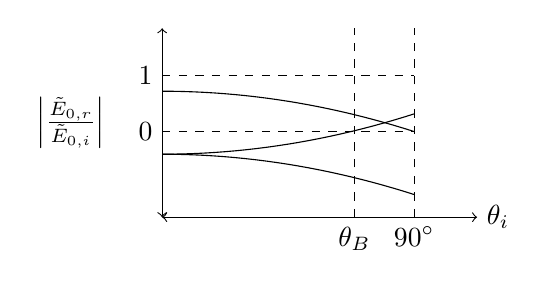
\begin{tikzpicture}[scale=0.4]
        \draw[<->] (0,0) -- (10,0);
        \node[right] at (10,0) {$\theta_i$};
        \draw[<->] (0,0) -- (0,6);
        \node[left] at (-1.5,3) {$\abs{\frac{\tilde{E}_{0,r}}{\tilde{E}_{0,i}}}$};
        \draw[dashed] (8,0) -- (8,6);
        \draw[dashed] (6.1,0) -- (6.1,6);
        \draw[dashed] (0,2.72) -- (8,2.72);
        \draw[dashed] (0,4.5) -- (8,4.5);
        \node[left] at (0,2.72) {$0$};
        \node[left] at (0,4.5) {$1$};
        \node[below] at (6.1,0) {$\theta_B$};
        \node[below] at (8,0) {$90^\circ$};
        \draw[domain=0:8] plot(\x, {0.02*\x*\x + 2});
        \draw[domain=0:8] plot(\x, {-0.02*\x*\x + 2});
        \draw[domain=0:8] plot(\x, {-0.02*\x*\x + 4});
    \end{tikzpicture}
    \caption{Plot of reflected/transmitted amplitudes, $\frac{n_2}{n_1} > 1$. Note that the upper one that is decreasing is the transmission amplitude that vanishes at $90^\circ$.}
    \label{5.1.Brewster}
\end{figure}
and \ref{5.1.TotalRef} for the $\frac{n_1}{n_2} < 1$ case
\begin{figure}[!h]
    \centering
    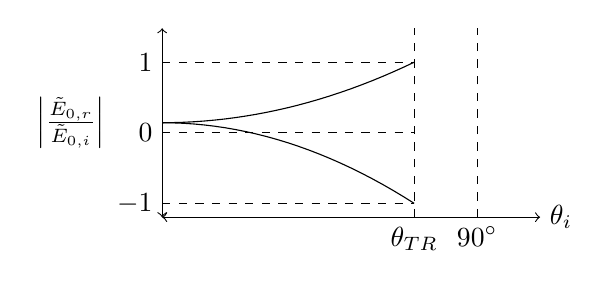
\begin{tikzpicture}[scale=0.4]
        \draw[<->] (0,0) -- (12,0);
        \node[right] at (12,0) {$\theta_i$};
        \draw[<->] (0,0) -- (0,6);
        \node[left] at (-1.5,3) {$\abs{\frac{\tilde{E}_{0,r}}{\tilde{E}_{0,i}}}$};
        \draw[domain=0:8] plot(\x, {0.03*\x*\x + 3});
        \draw[domain=0:8] plot(\x, {-0.04*\x*\x + 3});
        \draw[dashed] (8,0) -- (8,6);
        \node[below] at (8,0) {$\theta_{TR}$};
        \draw[dashed] (10,0) -- (10,6);
        \node[below] at (10,0) {$90^\circ$};
        \draw[dashed] (0,2.68) -- (8,2.68);
        \node[left] at (0,2.68) {$0$};
        \draw[dashed] (0,0.44) -- (8,0.44);
        \node[left] at (0,0.44) {$-1$};
        \draw[dashed] (0,4.92) -- (8,4.92);
        \node[left] at (0,4.92) {$1$};
    \end{tikzpicture}
    \caption{Plot of reflected/transmitted amplitudes for perp (top) and parallel (bottom) cases, $\frac{n_2}{n_1} < 1$.}
    \label{5.1.TotalRef}
\end{figure}

We then look at the energies of the transmission/reflection, and we first note $_jI = \expvalue{\vec{S}_j} = \frac{1}{2}\epsilon_j v_j E_j^2 \cos^2\theta_j$ which gives equations
\begin{align}
    R &= \frac{I_r}{I_i} =
    \begin{cases}
        \left( \frac{\alpha - \beta}{\alpha + \beta} \right)^2 & \text{parallel}\\
        \left( \frac{1 - \alpha \beta}{1 + \alpha \beta} \right)^2 & \text{perpendicular}
    \end{cases}\\
    T &= \frac{I_t}{I_i} =
    \begin{cases}
        \alpha \beta\left( \frac{2}{\alpha + \beta} \right)^2 & \text{parallel}\\
        \alpha \beta\left( \frac{2}{1 + \alpha \beta} \right)^2 & \text{perpendicular}
    \end{cases}
\end{align}

\chapter{5/6/14 --- EM waves in conducting media, frequency dependent $\epsilon$}

We begin with Maxwell's Equations in conductors
\begin{align}
    \vec{\nabla} \cdot \vec{E} &= \frac{\rho_f}{\epsilon} & \vec{\nabla} \cdot \vec{B} &= 0\\
    \vec{\nabla} \times \vec{E} + \pd{\vec{E}}{t} &= 0 & \vec{\nabla} \times \vec{B} &= \mu \sigma \vec{E} + \epsilon \mu \pd{\vec{E}}{t}
\end{align}
with $\vec{J}_f = \sigma \vec{E}$ already thrown in. 

First it is clear that there will be no $\rho_f$ inside the volume of the conductor, which we show by constructing $\pd{\rho_f}{t} = -\vec{\nabla} \cdot \vec{J} = -\sigma \vec{\nabla} \cdot \vec{E} = -\frac{\sigma}{\epsilon} \rho_f$ from the continuity equation. Then since $\sigma,\epsilon > 0$ we find $\rho_f \sim e^{-t/\tau}$ for $\tau = \frac{\epsilon}{\sigma}$, so characteristic decay time scale. Then if $\tau \ll T$ period of the wave, we have a good conductor, and if $\omega \tau \gg 1$ then we have a poor conductor.

Then if we plug each other together then we get
\begin{align}
    \nabla^2 \vec{E} &= \epsilon \mu \ptd{\vec{E}}{t} + \sigma \mu \pd{\vec{E}}{t}
\end{align}
with a similar $\vec{B}$ equation.

We will do the same thing as we did before, assume plane wave solutions
\begin{align}
    \vec{E}(\vec{r},t) &= \vec{E}_0 e^{i(\vec{k} \cdot \vec{r} - \omega t)} & \vec{B} &= \vec{B}_0 e^{i(\vec{K}\cdot \vec{r} - \omega t)}
\end{align}

We can again show that $\vec{k},\omega$ are the same so we won't go through that again. We note that their phase shift (recall $\vec{E}_0 \sim e^{iS}$ phase) may not be the same as we will later see. Then if we plug through our ansatz we find an imaginary term (due to the single derivative)
\begin{align}
    \vec{k} \cdot \vec{k} &= \epsilon \mu \omega^2 + i\sigma \mu \omega
\end{align}

We will define $\sqrt{\vec{k} \cdot \vec{k}} = k + i\kappa$ (note!! $k$ is not the magnitude of $\vec{k}$ but is just the real part!). Now let's define a bunch of crap $v_{\epsilon\mu} = \frac{1}{\sqrt{\epsilon \mu}}, k_{\epsilon\mu} = \frac{\omega}{v_{\epsilon\mu}}, \lambda = \frac{2\pi}{k_{\epsilon\mu}}$. Then we note that 
\begin{align}
    k &= k_{\epsilon\mu}\sqrt{\frac{\sqrt{1 + \frac{1}{\omega^2 \tau^2}}+1}{2}} & \kappa &= k_{\epsilon\mu}\sqrt{\frac{\sqrt{1 + \frac{1}{\omega^2\tau^2}}-1}{2}} = \frac{1}{\delta}\label{5.6.Ks}
\end{align}
where we define $\delta$ the skin depth, again the penetration of the wave. Then rewriting everything in terms of these variables (to lend some extra physical insight) we find
\begin{align}
    \vec{E}(\vec{r},t) &= \vec{E}_0 e^{-\hat{k} \cdot \vec{r}/\delta}e^{i(k\hat{k}\cdot \vec{r} - \omega t)}
\end{align}
and similarly for $\vec{B}$.

We then take a few limits. In the poor conductor limit, $\omega \tau \gg 1$, 
\begin{itemize}
    \item $k$ --- We can stare at \eqref{5.6.Ks} and note $k \to k_{\epsilon \mu}$.
    \item $\kappa$ --- $\kappa \to \frac{k_{\epsilon\mu}}{2\omega \tau}$, which we can also rewrite as $\kappa \to \frac{\sigma}{2}\sqrt{\frac{\mu}{\epsilon}} = \frac{Z_{\epsilon\mu}\sigma}{2}$ with again $Z_{\epsilon\mu} = \sqrt{\frac{\mu}{\epsilon}}$. 
    \item Skin depth ---  is then $\frac{2\omega \tau}{\kappa_{\epsilon\mu}} = \frac{2\tau}{T}\lambda_{\epsilon \mu}$ with again $\tau = \frac{\epsilon}{\sigma}$. 
\end{itemize}

And in the good conductor limit $\omega \tau \ll 1$
\begin{itemize}
    \item $k, \kappa \to k_{\epsilon\mu}\sqrt{\frac{1}{2\omega^2 \tau^2}} = \sqrt{\frac{\mu \sigma \omega}{2}}$.
    \item $\delta \to \sqrt{\frac{2}{\mu \sigma \omega}} = \frac{\lambda}{2\pi}$ so since the skin depth is smaller than a single wavelength then waves generally don't penetrate at all! This result is called the \emph{classical skin depth}. 
\end{itemize}

Then the overall picture is that where a good conductor has some currents and fields that float around exclusively on the surface, at a depth determined by the skin depth. 

We can then look at the fields. They look like
\begin{align}
    \vec{E}(\vec{r},t) &= \tilde{E}_0 \hat{n}_1 e^{-\hat{k}\cdot \vec{r}/\delta}e^{i(k \hat{k} \cdot \vec{r} - \omega t)} & \vec{B}(\vec{r},t) &= \frac{k + i\kappa}{\omega}\tilde{E}_0 \hat{k} \times \hat{n}_1e^{-\hat{k}\cdot \vec{r}/\delta}e^{i(k \hat{k} \cdot \vec{r} - \omega t)}
\end{align}
We then note that for $k + i\kappa = \mathcal{K}e^{i\phi}$ with $\mathcal{K} = k_{\epsilon \mu}\left( 1 + \left( \frac{\sigma}{\epsilon \mu} \right)^2 \right)^{1/4}$, then we find the phase shift of the two fields
\begin{align}
    \tan \phi &= \frac{\kappa}{k} = \sqrt{\frac{\sqrt{1 + \left( \frac{\sigma}{\epsilon \mu} \right)^2}-1}{\sqrt{1 + \left( \frac{\sigma}{\epsilon \mu} \right)^2}+1}}\\
    \frac{\tilde{B}_0}{\tilde{E}_0} &= \frac{k + i\kappa}{\omega} = \frac{e^{i\phi}}{v_{\epsilon\mu}}\left( 1 + \left( \frac{\sigma}{\epsilon \mu} \right)^2 \right)^{1/4}
\end{align}

These expressions are not very enlightening, but if we take the appropriate limits we find
\begin{itemize}
    \item Poor conductor --- $\frac{\tilde{B}_0}{\tilde{E}_0} \to \frac{1}{v_{\epsilon\mu}}$ because $\phi \to 0, \frac{\sigma}{\epsilon \mu} \to 0$.
    \item Good conductor --- $\frac{\tilde{B}_0}{\tilde{E}_0} \to \frac{e^{i\pi/4}}{v_{\epsilon \mu}}\sqrt{\frac{\sigma}{\epsilon \mu}} \gg \frac{1}{v_{\epsilon \mu}}$. Note then that the phase shift here is $\frac{\pi}{4}$, different from circuits' $\frac{\pi}{2}$, and $\vec{B}$ is enhanced by a factor of $\frac{\sigma}{\epsilon \mu}$, so in conductors $\vec{B}$ is relatively stronger than we see in regular media!
\end{itemize}

It is then natural to compute energy, Poynting vectors, etc. We find then (recalling an extra factor of $\frac{1}{2}$ by time averaging)
\begin{align}
    \expvalue{U} &= \frac{1}{4}\left( \epsilon \abs{\tilde{E}_0}^2 + \frac{1}{\mu}\abs{\tilde{B}_0}^2 \right)e^{-2\hat{k} \cdot \vec{r}/\delta}\\
    &= \frac{1}{4}\epsilon \frac{k^2}{k_{\epsilon \mu}^2}\abs{\tilde{E}_0^2 e^{-2\hat{k} \cdot \vec{r}/\delta}}\\
    \expvalue{\vec{S}} &= \frac{1}{2\mu }\Re\left( \expvalue{\vec{E}^* \times \vec{B}} \right) \\
    &= \frac{\hat{k}}{2} v_{\epsilon \mu} \epsilon \frac{\mathcal{K}}{k_{\epsilon \mu}} e^{-2\hat{k} \cdot \vec{r}/\delta}\cos\phi\\
    &= \frac{\hat{k}}{2} \frac{k_{\epsilon \mu}}{\epsilon}v_{\epsilon \mu}\expvalue{U}\\
    I = \expvalue{\abs{\vec{S}}} &= \frac{1}{2}\frac{k_{\epsilon \mu}}{k}v_{\epsilon \mu}\expvalue{U}
\end{align}

Phew!! Note the cool thing is that $\vec{S}$ has a phase shift again. These results are otherwise as we expect, with $\propto \hat{k} \cos \phi v_{\epsilon \mu}$ all factors we sort of expect.

Let's again take limits
\begin{itemize}
    \item Poor conductor $\omega \tau \gg 1$
        \begin{itemize}
            \item $\expvalue{ U} \to \frac{1}{2}\epsilon \abs{\tilde{E}_0}^2 e^{-2\hat{k} \cdot \vec{r}/\delta}$
            \item $\expvalue{\vec{S}} \to v_{\epsilon \mu} \expvalue{U}\hat{k}$
        \end{itemize}
        both of which are the same as nonconductor cases.
    \item Good conductor $\omega \tau \ll 1$
        \begin{itemize}
            \item $\expvalue{ U} \to \frac{1}{4}\epsilon \abs{\tilde{E}_0}^2 \frac{\sigma}{\epsilon \omega}e^{-2\hat{k}\cdot \vec{r}/\delta} = \frac{1}{4}\frac{\abs{\tilde{J}_0}\abs{\tilde{E}_0}}{\omega}e^{-2\hat{k}\cdot \vec{r}/\delta}$. Note that this has the overall form we want, $\vec{J} \cdot \vec{E}$ is a power dissipation (``Joule dissipation''), and we divide by $\omega$ to obtain the dissipation by the wave (on some intuitive level).
            \item $\expvalue{\vec{S}} \to \omega \delta \expvalue{U}\hat{k}$ and so we see that the power dissipation only occurs inside the skin depth. We can furthermore see this from the $U$ expression (up to some factors) is that when we integrate over the length of the wave $\hat{k} \cdot \vec{r}$ we pull out a factor of $\frac{\delta}{2}$, and so the power dissipated per unit area goes something like $\frac{\delta}{2} \abs{\tilde{J}_0}\abs{\tilde{E}_0}$ which shows that the wave is just a Joule dissipation inside the skin depth.
        \end{itemize}
\end{itemize}

Let's now look at the reflection/conducton at conducting surfaces (I'm dying\dots). Let's now rewrite our boundary conditions
\begin{align}
    \hat{n} \cdot \left[ \epsilon_1 \vec{E}_1 - \epsilon_2 \vec{E}_2 \right] &= \sigma_f & \hat{n} \cdot \left[ \vec{B}_1 - \vec{B}_2 \right] &= 0\\
    \hat{s} \cdot \left[ \vec{E}_1 - \vec{E}_2 \right] &= 0 & \hat{s} \cdot \left[ \frac{\vec{B}_1}{\mu_1} - \frac{\vec{B}_2}{\mu_2} \right] &= (\vec{K}_f \times \hat{n})\cdot\hat{s}
\end{align}

We can ignore the surface currents via $\vec{K}_f = 0$ because surface currents go with $\vec{E}$ and require a delta function, but since $\vec{E}$ goes at worst with $\frac{1}{r}$ (along a plane?) we note that no delta functions can crop up in $\vec{J}$ which means no surface currents.

We will also only consider normal incidence, because math is terrible otherwise. We will then take waveforms (take $\hat{u} \perp \hat{w} \perp \hat{k}$)
\begin{align}
    \vec{E}_i (\vec{r},t) &= \tilde{E}_{0,i} \hat{w}e^{i(k_i \hat{n} \cdot \vec{r} - \omega t)} &     \vec{B}_i(\vec{r},t) &= \frac{1}{v_i}\tilde{E}_{0,i}\hat{u}e^{i(k_t \hat{n} \cdot \vec{r} - \omega t)}\\
    \vec{E}_r (\vec{r},t) &= \tilde{E}_{0,r} \hat{w}e^{i(-k_r \hat{n} \cdot \vec{r} - \omega t)} &    \vec{B}_r(\vec{r},t) &= \frac{1}{v_i}\tilde{E}_{0,r}\hat{u}e^{i(k_t \hat{n} \cdot \vec{r} - \omega t)}\\
    \vec{E}_i (\vec{r},t) &= \tilde{E}_{0,t} \hat{w}e^{i(k_t \hat{n} \cdot \vec{r} - \omega t)}&     \vec{B}_t(\vec{r},t) &= \frac{1}{v_t}\tilde{E}_{0,t}\hat{u}e^{i(k_t \hat{n} \cdot \vec{r} - \omega t)}
\end{align}

We then note that our boundary conditions force (I think he's going through this algebra just to show us how it works, he's not actually expecting us to know/follow this) force
\begin{align}
    \tilde{E}_{0,i} + \tilde{E}_{0,r} &= \tilde{E}_{0,t}\\
    \frac{1}{\mu_1v_1}\left[ \tilde{E}_{0,i} - \tilde{E}_{0,r} \right] &= \frac{k_t + i\kappa_t}{\mu_2 \omega}\tilde{E}_{0,t}
\end{align}
for continuity of $\hat{s} \cdot \vec{E}, \hat{s} \times \vec{B}$ respectively.

We can then compute some stuff that he's not going to show and find (for some $\tilde{\beta} = \frac{\mu_1}{\mu_2}\frac{v_1}{\omega}(k_t + i\kappa_t)$)
\begin{align}
    \frac{\tilde{E}_{0,r}}{\tilde{E}_{0,i}} &= \frac{1 - \tilde{\beta}}{1 + \tilde{\beta}} & \frac{\tilde{E}_{0,t}}{\tilde{E}_{0,i}} &= \frac{2}{1 + \tilde{\beta}}
\end{align}

It is of note to point out some other ways to write $\tilde{\beta} = \beta \frac{k_t + i\kappa_t}{\omega / v_2} = \frac{Z_1}{Z_2} \frac{k_t + i\kappa_t}{k_2}$ for $\beta = \frac{\cos \theta_t}{\cos \theta_i}$ and $k_2 = \omega/v_2$.

We should now take our usual limits
\begin{itemize}
    \item Poor conductor --- $\tilde{\beta} \to \beta$ and we recover our nonconducting results for $\theta_i = 0$. 
    \item Good conductor --- $\tilde{\beta} \to \frac{\mu_1}{\mu_2}\frac{v_1}{\omega}\frac{1 + i}{\delta}$. Taking limits carefully then $\frac{\tilde{E}_{0,t}}{\tilde{E}_{0,i}} \ll 1$ and $\frac{\tilde{E}_{0,r}}{\tilde{E}_{0,i}} = -1$. The former will be considered in greater detail on a PS (WTF) where we will consider higher order terms by treating the conductor as a dielectric with complex $\epsilon$ (just a preview), and the latter is what we expect for bouncing a wave off a boundary such that the boundary condition forces $E = 0$ at the boundary.
\end{itemize}

We can examine now a crude model of the frequency-dependent $\epsilon$ phenomenon that we sometimes see. Let's consider an electron bound by some binding force $F_b = -m\omega_0^2x$, always a valid approximation if we expand about a minimum. We can also model some damping force $F_d = -m\gamma \pd{x}{t}$. Lastly we can write down the driving force on the electron due to the electromagnetic wave $F_e = qE_0\cos\omega t$.

We can then solve this equation of motion, going to complex exponentials, and we find (using $\tilde{X}(t) = \tilde{X}_0e^{-i\omega t}$)
\begin{equation}
    \tilde{X}_0  = \frac{q/m}{\omega_0^2 - \omega^2 - i\gamma \omega}\tilde{E}_0
\end{equation}

We can then compute the dipole moment that this produces 
\begin{equation}
    \vec{p}(t) = q\vec{X}(t) = \frac{q^2/m}{\omega_0^2 - \omega^2 - i\gamma \omega}\tilde{E}_0 e^{-i\omega t}
\end{equation}

We can then take this and compute dielectric constant! We first compute polarization density by summing over all the dipoles, with some $f_j$ in the below sum being the number of electrons with binding $\omega_j$ and damping $\gamma_j$ per site and $N$ number of sites per unit volume, so
\begin{align}
    \vec{P} &= \frac{Nq^2}{m}\left( \sum_{j}^{}\frac{f_j}{\omega_j^2 - \omega^2 - i\gamma_j\omega} \right)\vec{E}
\end{align}

We furthermore know though that $\vec{P} = \tilde{\chi}_e \epsilon_0 \vec{E}$ where we allow $\tilde{\chi}$ to be complex. Then $\tilde{\epsilon}_r = 1 + \tilde{\chi}_e$ which is just
\begin{align}
    \tilde{\epsilon}_r &= 1 + \frac{Nq^2}{\epsilon_0m}\sum_{j}^{}\frac{f_j}{\omega_j^2 - \omega^2 - i\gamma_j\omega}\label{5.6.diel}
\end{align}

Now that we have some dielectric constant, let's see what happens when we plug this thorugh Maxwell equations (we will assume $\mu_0$ for simplicity)
\begin{align}
    \nabla^2 \vec{E} &= \tilde{\epsilon}\mu_0 \ptd{\vec{E}}{t}
\end{align}

The under complex permittivity and conductivity cases we found the following two equations \eqref{5.6.CPerm} and \eqref{5.6.cond} respectively
\begin{align}
    \left(\vec{k} \cdot \vec{k}\right) \vec{E}_0 e^{i\left( \vec{k} \cdot \vec{r} - \omega t \right)} &= \tilde{\epsilon}\mu_0 \omega^2 \vec{E}_0 e^{i\left( \vec{k} \cdot \vec{r} - \omega t \right)}\label{5.6.CPerm}\\
    &= \left( \epsilon \mu \omega^2 + i\sigma \mu \omega \right)\vec{E}_0 e^{i\left( \vec{k} \cdot \vec{r} - \omega t \right)}\label{5.6.cond}
\end{align}

Then again we define $\vec{k} \cdot \vec{k} = \tilde{\epsilon} \mu_0 \omega^2$ and we assumed $\abs{k}^2 = k + i\kappa$, and so we set equal $k + i\kappa = \sqrt{\tilde{\epsilon}\mu_0 \omega^2}$.

We then refer back to $\tilde{\epsilon}$ given by \eqref{5.6.diel} and plug this through what we have above. Assuming then $N \ll 1$ dilute system we can expand the square root in a series expansion and we will finally find
\begin{align}
    k + i\kappa &= \omega \sqrt{\epsilon_0 \mu_0}\left[ 1 + \frac{1}{2}\frac{Nq^2}{m\epsilon_0}\sum_{j}^{}\frac{f_j}{\omega_j^2 - \omega^2 - i\gamma_j \omega} \right]\\
    n &= \frac{c}{v} = \frac{c}{\omega/k} = \frac{ck}{\omega} = 1 + \frac{Nq^2}{2m\epsilon_0}\sum_{j}^{}\frac{f_j(\omega_j^2 - \omega^2)}{(\omega_j^2 - \omega^2)^2 + (\gamma_j \omega)^2}\\
    \kappa &= \frac{\omega^2}{c}\frac{Nq^2}{2m\epsilon_0}\sum_{j}^{}\frac{\gamma_j f_j}{\left( \omega_j^2 - \omega^2 \right)^2 + \left( \gamma_j \omega \right)^2}
\end{align}

We will finish this approximation next class, just summing over all the oscillators, but we have an explicit expression for $n,\kappa$ the speed and skin depth of the light in media just by this model!
\chapter{5/8/14 --- Transmission Lines}

Recall that last class we left off with expression
\begin{align}
    k + i\kappa &= \sqrt{\tilde{\epsilon}\mu_0 \omega^2} = \frac{\omega}{c}\sqrt{\frac{\tilde{\epsilon}}{\epsilon_0}} = \frac{\omega}{c} \left[ 1 + \frac{1}{2}\frac{Nq^2}{m\epsilon_0}\sum_{_i}^{}\frac{f_i}{\omega^2 - \omega_j^2 - i\delta_j\omega} \right]\\
    n &= \frac{ck}{\omega} = 1 + \frac{Nq^2}{2m\epsilon_0}\sum_{_i}^{}\frac{f_i(\omega^2 - \omega_j^2)}{(\omega^2 - \omega_j^2)^2 + \delta_j^2\omega^2}\\
    \kappa &= \frac{\omega^2}{c}\frac{Nq^2}{2m\epsilon_0}\sum_{_i}^{}\frac{f_i\gamma_j}{(\omega^2 - \omega_j^2)^2 + \delta_j^2\omega^2}
\end{align}

Let's now take some limits. 
\begin{itemize}
    \item In the low-frequency limit $\omega \ll \omega_j$
        \begin{align}
            n &\to 1 + \frac{Nq^2}{2m\epsilon_0} \sum_{j}^{}\frac{f_j}{\omega_j^2 - \omega^2} = 1 + \frac{Nq^2}{2m\epsilon_0}\sum_{j}^{}\frac{f_j}{\omega_j^2}\left( 1 + \frac{\omega^2}{\omega_j^2} \right)\\
            &= 1 + A\left( 1 + \frac{B}{\lambda^2} \right)
        \end{align}
        This $A$ term is called the \emph{coefficient of refraction}, the refraction at low frequencies solely due to the resonances, and $B$ (dependent on $\omega^2$) is the \emph{coefficient of dispersion} because it relates $\omega$ to $n$. 
    \item Conductor limit $\omega_0 = 0, \omega \ll \omega_j$ then
        \begin{align}
            \frac{\tilde{\epsilon}}{\epsilon_0} = 1 + \frac{Nq^2}{\epsilon_0}\sum_{j}^{} \frac{f_j}{k_j} + i\frac{N_e q^2}{\epsilon_0 m}\frac{1}{\gamma_0 - i\omega}\frac{1}{\omega} + O(\omega^2)
        \end{align}
        with $N_e = Nf_0$ the number of free conduction electrons, as $\omega_0 \to 0$ gives $k_0 \to 0$. If we compare this with our previous expression for $\vec{k} \cdot \vec{k}$
        \begin{align}
            \vec{k} \cdot \vec{k} &= \epsilon \mu_0 \omega + i\sigma\mu_0\omega\\
            &= \left( \epsilon + \frac{i\sigma}{\omega} \right)\mu_0\omega^2
        \end{align}
        then we can identify $\sigma = \omega \Im(\tilde{\epsilon}) = \frac{N_e q^2}{m}\frac{1}{\gamma_0 - i\omega}$. And if we examine in the limit of $\gamma_0 \gg \omega$ then we identify $\boxed{\sigma = \frac{N_eq^2}{m}}$.

        Recall then that we defined the damping force such that $\frac{1}{\gamma} = \frac{v}{\abs{F_d/m}}$. Then if we plug this against the Drude model for conductivity $\sigma = \frac{N_eq^2\lambda_{mfp}}{2mv_t}$ for mean free path $\lambda$ and thermal $v$, then we find that
        \begin{equation}
            \frac{d}{F_d/m} = \frac{1}{\gamma} = \frac{2m\sigma}{N_eq^2} = \frac{\lambda_{mfp}}{v_t}  = \frac{\tau}{2}
        \end{equation}
        The takeaway of this crude model is just that we can model condutivity either by plugging Ohm's Law through Maxwell equations (apparently as we've done before though this escapes me atm) or by introducing a complex dielectric constant.
    \item High frequency limit, or plasma limit, $\omega \gg \omega_j$ gives
        \begin{align}
            n \to 1 - \frac{Nq^2}{m\epsilon_0}\sum_{j}^{}\frac{f_j}{\omega^2} = 1 - \frac{\omega_p^2}{\omega^2}
        \end{align}
        for $\omega_p^2 = \frac{Nq^2}{m\epsilon_0}\sum_{j}^{}f_j$. We then note that $n < 1$ thankfully.

        It turns out that even at lower frequencies the plasma limit is applicable; note that there is no reason that this should work other than empiricism. We can see that for $\omega_p > \omega$ then we have negative dielectric constant, which gives no propagating wave and therefore total internal reflection. This gives a field penetrating depth $\delta = \kappa = \frac{\omega_p}{c}$. This is actually why metals reflect light, because of their high $N$ and high $\omega_p$ yielding total internal reflection on the surface! (there might be a few incorrect factors of $2$ in the math, since he did it wrong on the board and didn't bother correcting everything after somebody pointed it out\dots)
\end{itemize}

Let's now look at guided waves. We will do a transmission line today. Let's place a current $I$, voltage $V$, and charge $Q$ at a location $z$ along the transmission line, place $I + dI, V+dV, Q+dQ$ at $z + dz$, let the transmission line be completely anti-symmetric ($-I$, etc. on the bottom), and let it exhibit inductance $\mathcal{L}$ and apacitance $\mathcal{C}$. Yeah, a lot of specifications, but pretty intuitive labels.

Let's now examine what happens to the change in charge. Note that by our assumptions the difference in voltage across the transmission line is $2V$, so by the definition of capacitance $dQ =Cdz d(\Delta V) = 2CdzdV$. This is also a result of mismatched currents, which produces 
\begin{align}
    -dI dt &= d(\Delta V) \mathcal{C} dz\\
    \pd{I}{z} &= -\mathcal{C}\pd{\Delta V}{t}
\end{align}

We can also compute what happens due to inductance. This is just
\begin{align}
    \frac{1}{2}d(\Delta V) &= -\frac{\mathcal{L}}{2} dz \pd{I}{t}\\
    \pd{\Delta V}{z} &= -\mathcal{L}\pd{I}{t}
\end{align}

Decoupling these two equations we find
\begin{align}
    \ptd{I}{z} &= \mathcal{L}\mathcal{C}\ptd{I}{t} & \ptd{\Delta V}{z} &= \mathcal{LC}\ptd{\Delta V}{t}
\end{align}

We then find that if $I_{\pm}(z,t) = F\left( \pm \frac{\omega}{v}z - \omega t \right)$ some general current moving either direction (and $F$ a general function) then we know that $\Delta V = Z_{\pm}I_\pm$. We can plug these back into the EOM and find ($u = \left( \pm \frac{\omega}{v}z - \omega t \right)$)
\begin{align}
    \pm I_{\pm}\frac{\omega}{v}\pd{F}{u} &= -\mathcal{C}Z_{\pm}I_{\pm}\omega \pd{F}{u}\\
    Z_{\pm} &= \pm \frac{1}{v\mathcal{C}} = \sqrt{\frac{\mathcal{L}}{\mathcal{C}}}
\end{align}

We then define this quantity $Z_{\mathcal{LC}} = \sqrt{\frac{\mathcal{L}}{\mathcal{C}}}$ the \emph{characteristic impedance}.

Let's do an example. Consider coaxial cable, $\mathcal{C} = \frac{2\pi \epsilon}{\ln \frac{b}{a}}, \mathcal{L} = \frac{\mu \ln \frac{b}{a}}{2\pi}$. Then we find $v = \frac{1}{\sqrt{LC}}$ which we know by HW4 (due today) is equal to $\frac{c}{n}$. Moreover then 
\begin{equation}
    Z_{\mathcal{LC}} = \frac{\ln \frac{b}{a}}{2\pi}\sqrt{\frac{\mu}{\epsilon}} = \frac{\ln \frac{b}{a}}{2\pi}Z_{\mu \epsilon}
\end{equation}

Then if we compute for some reasonable $\frac{b}{a}\sim1$ then we find the characteristic impedance of coax cables is about $50\Omega$. 

We can also examine a stripline, two long parallel plates. Note that $\mathcal{C} = \frac{\epsilon w}{h}$ and $\mathcal{L} = \frac{\mu h}{w}$ with $h$ the separation and $w$ the width, both per unit length. Again $v = \frac{c}{n}$ as before (we can check this using the capacitance/inductance we calculated here), and it turns out that $Z_{\mathcal{LC}} = \sqrt{\frac{\mathcal{L}}{\mathcal{C}}} = \frac{h}{w}Z_{\mu \epsilon}$. 

Time to consider an arbitrary case, arbitrary electrodes! Let's exhibit two arbitrary electrodes in space with $\epsilon,\mu$, with $\sigma \to \infty$ (so charges/currents only on surface). Let's write the general form of the stuff for this setup that would look like transmission line
\begin{align}
    \vec{E} &= \left[ \hat{x}E_x(x,y) + \hat{y}E_{y}(x,y) \right]e^{i(kz - \omega t)}\\
    \vec{E} &= \left[ \hat{x}B_x(x,y) + \hat{y}B_{y}(x,y) \right]e^{i(kz - \omega t)}\\
    \vec{E} &= \rho_0(x,y)e^{i(kz - \omega t)}\\
    \vec{E} &= \hat{z}J_z(x,y)e^{i(kz - \omega t)}
\end{align}

What we will show is exactly what the equations look like, that the $x,y$ components of the field. Let's look at the Maxwell Equations then (sorry if these notes don't make sense, I'm so tired today for some reason)
\begin{align}
    [\vec{\nabla} \times \vec{E}]_z &= -\pd{\vec{B}}{t} \cdot \hat{z} &\Rightarrow \pd{E_y}{x} - \pd{E_x}{y} &= 0\\
    \vec{\nabla} \cdot \vec{E} &= \frac{\rho}{\epsilon} &\Rightarrow \pd{E_x}{x} + \pd{E_y}{y} &= \frac{\rho(x,y)}{\epsilon}\\
    [\vec{\nabla} \times \vec{B}]_z &= \mu \vec{J}_f \cdot \hat{z} + \epsilon \mu \pd{\vec{E}}{t}\cdot \hat{z} &\Rightarrow \pd{B_x}{y} - \pd{B_y}{x} &= \mu J_z (x,y)\\
    \vec{\nabla} \cdot \vec{B} &= 0 &\Rightarrow \pd{B_x}{x} + \pd{B_y}{y} &= 0
\end{align}

These equations are what justify the general forms we wrote above, because our forms satisfy these, and these are the constraints for transmission line-like propagation. We can then examine the remaining four Maxwell Equations (other components of the curls) and note that this implies
\begin{align}
    \vec{B} &= \frac{1}{v}\hat{k}\times \vec{E}\\
    \hat{x}B_x + \hat{y}B_y &= \frac{1}{v}\left( -x E_y + \hat{y}E_x \right)
\end{align}
which shows that our wave is fully determined by $E_{x,y}$. Goodies!

We then apply continuity. We know that $\vec{\nabla} \cdot \vec{J} = -\pd{\rho}{t}$. This then gives us using our forms $J_0 = v\rho_0$. The transmission line limit then looks like $\Delta V = \int d\vec{l} \cdot \vec{E}$ and $\vec{K} = \oint dl\; \vec{K}$ (the second is a line integral because currents are only on the surface, recall), so if we integrate we can find
\begin{align}
    I &= v \oint dl\; \sigma_0 = \epsilon v \oint dl \;\hat{n} \cdot \vec{E}
\end{align}
so that both $I,\Delta V$ are written in terms of $\vec{E}$! Then we note
\begin{align}
    Z &= \frac{\Delta V}{I} = Z_{\epsilon \mu}\frac{\oint dl\; \hat{n} \cdot \vec{E}}{\int d\vec{l} \cdot \vec{E}}
\end{align}
but we already now from our HW that (he's just flaunting the fact that I haven't figured out that problem yet, jerk)
\begin{equation}
    Z = Z_{\mathcal{LC}} = \sqrt{\frac{\mathcal{L}}{\mathcal{C}}} = \mathcal{L}\sqrt{\frac{1}{\mu \epsilon}} = \frac{\mathcal{L}}{\mu_0}Z_{\epsilon \mu}
\end{equation}
which comparing with above shows that the retaio of the integrals is just $\mathcal{L}/\mu_0$.
\chapter{5/13/14 --- Transmission line junctions, Waveguides}

Recall that transmission lines have \begin{align}
    \Delta V(z,t) &= V_0e^{i(kz - \omega t)}\\
    I(z,t) &= I_0e^{i(kz - \omega t)}\\
    V_0 &= Z_{\epsilon\mu} I_0
\end{align}
with $Z_{\epsilon \mu} = \sqrt{\frac{\mu}{\epsilon}}$. We note that in this case, without resistance, the voltage and current are in phase.

Let's then compute the energy and power of the transmission line
\begin{align}
    \expvalue{\vec{S}} &= \frac{1}{2\mu}\Re\left( \expvalue{\vec{E}^* \times \vec{B}} \right) = \hat{k}\frac{1}{2\mu v_{\mu \epsilon}} \abs{E_0}^2\\
    &= \frac{1}{2}\hat{k}\epsilon v_{\mu\epsilon}\abs{E_0}^2 = \hat{k}v_{\mu \epsilon} \expvalue{U}
\end{align}
with $v_{\mu\epsilon} = \frac{1}{\sqrt{\mu \epsilon}} = \frac{1}{\sqrt{LC}}$. We also compute power
\begin{align}
    P &= \int\limits_{S}^{}da\;\hat{z} \cdot \expvalue{\vec{S}} = \frac{1}{2}v_{\mu\epsilon} \int\limits_{S}^{}da\;\epsilon \abs{E_0}^2\\
    &= \frac{1}{2}v_{\mu \epsilon}C\abs{V_0}^2 = \frac{1}{2}\sqrt{\frac{C}{L}}\abs{V_0}^2\\
    &= \frac{1}{2}\frac{\abs{V_0}^2}{Z_{LC}} = \frac{1}{2}\Re\left( I_0^* V_0 \right)
\end{align}
with $Z_{LC} = \frac{L_0}{\mu_0}\sqrt{\frac{\mu}{\epsilon}} = \sqrt{\frac{L}{C}}$ and these are all per unit lengths. We can anticipate the phase difference case between $I,V$ by writing it in terms of real part, but without resistance it's just a direct product of the amplitudes. On the homework, we will introduce a resistance, but obviously this will result in a power dissipation.

Let's see what happens when we join two wires of different impedances, so the reflection/transmission at a junction. We will assume two coaxial cables of impedances $Z_1, Z_2$ connected at $z=0$ the coordinate, and so if we assume wave solutions
\begin{align}
    V_<(z,t) &= e^{i(k_1z - \omega t)} + \tilde{r}e^{i(k_1r + \omega t)}\\
    I_<(z,t) &= \frac{V_<(z,t)}{Z_1}\\
    V_>(z,t) &= \tilde{t}e^{i(k_2z - \omega t)}\\
    I_>(z,t) &= \frac{V_>(z,t)}{Z_2}
\end{align}

Note that they share $\omega = k_iv_i$. We then require that the BCs match, so $V_{<} = V_{>}$ gives $1 + \tilde{r} = \tilde{t}$, and matching current gives $\frac{1 - \tilde{r}}{Z_1} = \frac{\tilde{t}}{Z_2}$. Solving these two equations produces
\begin{align}
    \tilde{r} &= \frac{Z_2 - Z_1}{ Z_2 + Z_1} & \tilde{t} &= \frac{2Z_2}{Z_2 + Z_1}
\end{align}

This gives us expressions for our reflected and transmitted power
\begin{align}
    R &= \frac{1}{2}\frac{\abs{\tilde{r}}^2}{\frac{1}{2}\frac{1}{Z_{1}}} = \abs{\frac{Z_2 - Z_1}{Z_2 + Z_1}}^2 & T &= \frac{\frac{1}{2}\frac{\abs{\tilde{t}^2}}{Z_2}}{\frac{1}{2}\frac{1}{Z_1^2}} = \frac{Z_1}{Z_2}\left( \frac{2Z_2}{Z_1 + Z_2} \right)^2
\end{align}

Note that we are still only working with real $Z$, which will need to be generalized (of course on the homework). 

Let's look at some examples; what if we terminate in a load? The setup actually looks exactly like before but instead of a wire at $Z_2$ we have a load at $Z_{L}$ for load. Then for a dissipationless transmission line we can choose $Z_L = Z_1$ which actually produce no reflection; this is \emph{impedance matching}. Since we have only considered real $Z_1$ we thusfar need a resistor to impedance match. 

Let's now consider a somewhat more complicated case. Recall that when we joined two transmission lines we assumed that there was no wave coming at the junction in $Z_2$. We can consider instead the case where we attach a $Z_L$ at the end of $Z_2$ wire,such that $Z_L\neq Z_2$ (else impedance matching produces no reflection and no interesting). We will try to determine a $Z(l)$ that encapsulates both $Z_2, Z_L$ given that $Z_2$ has length $l$. 

{\em \small The overall look of our approach will be to determine $Z$ as a function of $z$ for an arbitrary set of incident and reflected waves in $Z_2$, then match the boundary condition that $Z(l) = Z_L$ the load. We can then compute what $Z$ at the junction $Z(0)$ looks like, and this will tell us how reflection/transmission look at the junction}

Let's assume right and left going wave (in $Z_2$) $V_+, V_-$ respectively. Let's define the ratio of the two waves $r(z) = \frac{V_-}{V_+}$. 

We note then that $V(z) = V_+ + V_- = V_+(z)\left[ 1 + r(z) \right]$ and $I(z) = \frac{V_+}{Z_{LC}} - \frac{V_-}{Z_{LC}} = \frac{V_+}{Z_{LC}}\left( 1 - r(z) \right)$. Then the impedance of the transmission line looks like
\begin{equation}
    Z(z) = \frac{V}{I} = Z_{LC} \frac{1 + r(z)}{1 - r(z)}
\end{equation}

We then note that if there were no reflection then $r = 0$ and we recover the standard $Z(z) = Z_{LC}$ result. Recall then that $V_+ = V_+(0) e^{ikz}, V_- = V_-(0)e^{-ikz}$ which gives that $r(z) = r(0)e^{-2ikz}$ and so that
\begin{equation}
    Z_1 = Z_{LC} \frac{1 + r(0)e^{-2ikz}}{1 - r(0)e^{-2ikz}}
\end{equation}

Lastly we impose that $Z(l) = Z_L$, the matching condition at the end of the line, so then we can solve $r(0) = e^{2ikl}\frac{\frac{Z_L}{Z_{LC}} - 1}{\frac{Z_L}{Z_{LC}} + 1}$.

We are also interested in $Z(0)$ the impedance at the junction, which is just 
\begin{equation}
    Z(0) = Z_{LC}\frac{1 + r(0)}{1 - r(0)} = Z_{LC}\frac{Z_L - iZ_{LC}\tan kl}{Z_{LC} - iZ_2\tan kl}
\end{equation}
where the $\tan$ terms pop pop out of some algebra with the exponents.

Let's then examine some limits. Consider a short circuit $Z_L = 0$, then $Z_1 = -iZ_{LC}\tan kl$. Then supposing that if $2n\frac{\lambda}{4} < l < (2n+1)\frac{\lambda}{4}$ then $\tan > 0$ and we find that $Z(0)$ is a negative imaginary number, which looks inductive. On the other hand, if we're in the other half of the lengths, then $\tan < 0$ and we have a positive imaginary number for $Z(0)$ which looks capacitive.

If then $l = \frac{\lambda}{4}$ (plus some $2\pi\lambda$s) then $kl = \frac{\pi}{2}$ and $Z(0) = \frac{Z_{LC}^2}{Z_L}$ which looks just like a transformer, taking the impedance from one value to another (I missed the explanation). Moreover if $l = \frac{\lambda}{2}$ then $kl=\pi$ and $Z(0) = Z_L$. 

Let's now consider wave guides. Consider a translationally symmetric hunk of metal surrounded by conductor. We will find that the fields inside are no longer perfectly transversee, and the speed of the wave depends on $\omega$. Let's write down the Maxwell Equations in this waveguide. We will assume waveforms
\begin{align}
    \vec{E}(\vec{r},t) &= \vec{E}_0(\vec{r}_{\perp}) e^{i(kz - \omega t)} & \vec{B}(\vec{r},t) &= \vec{B}_0(\vec{r}_{\perp}) e^{i(kz - \omega t)}
\end{align}
for $\vec{r}_{\perp} = x\hat{x} + y\hat{y}$. We note that the Maxwell equations, taking some curls (such as $(\vec{\nabla}\times \vec{E})_z \propto B_z$) shows that everything can be written solely in terms of the $z$ components of the $\vec{E}, \vec{B}$ fields as below
\begin{align}
    \vec{B}_{0,\perp} &= \frac{1}{k_{\epsilon \mu}^2 - k^2}\left[ ik\vec{\nabla}_{\perp}B_{0,z} + i\frac{k_{\epsilon\mu}}{v_{\epsilon \mu}}\hat{z}\times \vec{\nabla}_{\perp}E_{0,z} \right]\\
    \vec{E}_{0,\perp} &= \frac{1}{k_{\epsilon \mu}^2 - k^2}\left[ ik\vec{\nabla}_{\perp}E_{0,z} - ik_{\epsilon\mu}v_{\epsilon \mu}\hat{z}\times \vec{\nabla}_{\perp}B_{0,z} \right]
\end{align}

We can identify that $\vec{\nabla} \cdot \left( \hat{z} \times \vec{\nabla}_{\perp} \right) = 0$ through some algebra, so we will curl both of these fields to obtain eigenvalue/eigenvector equations
\begin{align}
    0 = \vec{\nabla} \cdot \vec{E} &= e^{i(kz - \omega t)}\left( \vec{\nabla}_{\perp} \cdot \vec{E}_{0,\perp} + ikE_{0,z} \right)\\
    &= \frac{ik}{k_{\epsilon \mu}^2 - k^2}\nabla^2_{\perp} E_{0,z} + ikE_{0,z}\\
    &= \nabla^2_{\perp} E_{0,z} + E_{0,z}\left(k_{\epsilon \mu}^2 - k^2\right)
\end{align}

This then looks like an eigenvalue equation! Recall that $k_{\epsilon \mu} = \frac{\omega}{v_{\epsilon \mu}}$. We will typically solve for separate modes
\begin{itemize}
    \item TE modes --- Transverse electric, set $E_{0,z} = 0$ and find solutions to $B_{0,z}$ equation
    \item TM modes --- Transverse magnetic, set $B_{0,z} = 0$ and find solutions to $E_{0,z}$ equation
    \item TEM modes --- transverse electric and magnetic, set both $E_{0,z}, B_{0,z} = 0$. This then looks exactly like a transmission line, which we've already solved
\end{itemize}

Of course we cannot solve the eigenvalue problem without some BCs. We assume that the waveguides are surrounded by perfect conductors, so that $\vec{E} + \vec{B}$ vanish inside the conductor. This gives us BCs on the normal/tangential components. 
\begin{itemize}
    \item By $\vec{\nabla} \cdot \vec{B} = 0$ we find that $\hat{n} \cdot \vec{B} = 0$. 
    \item Examining next Faraday's Law we can find that $\hat{z} \cdot \vec{E} = E_{0,z} = 0, \hat{t} \cdot \vec{E} = E_{0, \perp} = 0$ with $\hat{t} \perp \hat{n}, \hat{z}$.
    \item Recalling our expression for $\vec{E}_{0,\perp}$ we can plug in and find that $\hat{t} \cdot \vec{\nabla}_{\perp} E_{0,z} = 0$ and that $\hat{n} \cdot \vec{\nabla}_{\perp}B_{0,z} = 0$.

\end{itemize}
\chapter{5/20/14 --- Waveguides}

We will need a makeup lecture because we missed the last lecture due to ditch day (thank god he's not going to try to cram, this class can't go any faster).

Recall that when we applied the Maxwell equations to waveguides we found that longitudinal components popped up such that
\begin{align}
    \nabla^2_{\perp}E_{0,z} + (k_{\epsilon \mu}^2 - k^2)E_{0,z} &= 0\label{5.20.MEs}\\
    \nabla^2_{\perp}B_{0,z} + (k_{\epsilon \mu}^2 - k^2)B_{0,z} &= 0\\
    \vec{B}_{0,z} &= \frac{1}{k_{\epsilon \mu}^2 - k^2}\left[ ik\vec{\nabla}_{\perp} B_{0,z} + i\frac{k_{\epsilon \mu}}{v_{\epsilon \mu}}\hat{z} \times \vec{\nabla} _{\perp}E_{0,z} \right]\\
    \vec{E}_{0,z} &= \frac{1}{k_{\epsilon \mu}^2 - k^2}\left[ ik\vec{\nabla}_{\perp} E_{0,z} - ik_{\epsilon \mu}v_{\epsilon \mu}\hat{z} \times \vec{\nabla} _{\perp}B_{0,z} \right]
\end{align}
with $v_{\epsilon \mu} = \frac{1}{\sqrt{\epsilon \mu}}$ and $k_{\epsilon \mu} = \frac{\omega}{v_{\epsilon \mu}}$. There were then three modes, TE (set $E_{0,z} = 0$), TM (set $B_{0,z} = 0$), and TEM which is what we what we've already considered, both have no longitudinal components.

We also showed that the BCs were that
\begin{align}
    E_{0,z}\Bigg|_C &= 0 & \hat{n} \cdot \vec{\nabla}_{\perp}B_{0,z} \Bigg|_C &= 0
\end{align}

Lastly we define a $\hat{n} \perp C$ normal to the boundary.

We can first show that there are no TEM modes in a hollow waveguide, theorem. Consider the Maxwell equations, but recalling $E_z, B_z =0$
\begin{align}
    0 &= \vec{\nabla} \cdot \vec{E} = \pd{E_x}{x} + \pd{E_y}{y} + \left( \pd{E_z}{z} = 0 \right)\\
    0 = B_{0,z} &= \left[\vec{\nabla} \times \vec{E}\right]_z = \pd{E_y}{x} - \pd{E_x}{y}\\
    \vec{\nabla} \times \vec{E} &= 0
\end{align}

Then from $\vec{\nabla} \times \vec{E} = 0$ we note that $\vec{E} = -\vec{\nabla} \phi$ and since the inside of the waveguide is hollow (conductor) we satisfy  Laplace's equation inside the waveguide which means that we exhibit averaging inside the waveguide and that the surface is an equipotential, making the waveguide itself an equipotential. This implies that no current can flow. The intuitive way to see this is that all TEM modes need two electrodes (think transmission lines) but a hollow waveguide is a single sheet of surface so there's nowhere for the ``voltage drop'' to occur that corresponds to a current.

Let's tnow look at TM modes. We set $B_{0,z} = 0$, so we have some wave equation for $E_{0,z}$. Define then $\psi = E_{0,z}$, then $\nabla^2_{\perp} \psi + \gamma^2 \psi = 0$ with $\gamma^2 = k_{\epsilon \mu}^2 - k^2$, and recalling that $\psi(\in C) = 0$ (vanishing on boundary). Then the eigenfunctions have eigenvalues and we have boundary conditions so we can solve out. Then we also know $E_{0,z} = \psi_n(x,y)$ and $\vec{B}_{0,\perp} = \frac{ik}{\gamma_n^2}\vec{\nabla}_{\perp}\psi_n$ and $E_{0,\perp} = -v_{\epsilon \mu} \frac{ik_{\epsilon \mu}}{\gamma_n^2}\hat{z} \times \vec{\nabla}_{\perp}\psi_n$ (he's just plugging into our \eqref{5.20.MEs} I think). Then we can take 
\begin{equation}
    \omega^2 = v_{\epsilon \mu}^2 k_{\epsilon \mu}^2 = v_{\epsilon \mu}^2\left( \gamma_n^2 + k^2 \right)\end{equation}
by plugging in our equation for $\gamma$ and then we find that there's a cutoff frequency at $\omega_{\epsilon\mu} = v_{\epsilon \mu}\gamma_n$! This differs from the TEM mode result which was just $\omega = v_{\epsilon \mu}k$. Note that if the frequency is below the cutoff frequency we exhibit attenuation because imaginary $k$, which we can compute.

Note that each mode within the waveguide has its own dispersion relation! The asymptotic behaviors though are that $k(\omega \to \infty) \to k_{\epsilon \mu}$ and that $v_n(\omega \to \omega_{\epsilon \mu}) \to \infty$. 

We then look at the wave impedance, which is just (note that while in general $\frac{\vec{B}}{\mu} = \frac{1}{Z}\hat{k} \times \vec{E}$ doesn't hold, it still holds for the transverse components)
\begin{equation}
    \vec{H}_{0,\perp} = \frac{1}{Z}\hat{k} \times \vec{E}_{0, \perp}
\end{equation}
giving $Z = \frac{\abs{\hat{k} \times \vec{E}_{0,z}}}{\abs{\vec{H}_{0,z}}}$. Then we see that 
\begin{equation}
    Z_n^{TM}(\omega) = \frac{k_n^{TM}(\omega)}{k_{\epsilon \mu}} \sqrt{\frac{\mu}{\epsilon}} = Z_{\epsilon \mu}\sqrt{1 - \frac{\omega_{\epsilon \mu}^2}{\omega^2}}
\end{equation}

This then goes to a short circuit as $\omega \to \omega_{\epsilon \mu}$. Note that the TE modes we will not do separately, but it in fact will exhibit complementary behavior, so instead of $k \to 0$ at cutoff, $k \to \infty$, and at cutoff $v_n \to 0$ and the circuit looks like an open circuit instead of a short.

Let's do an example (thankfully). Let's exhibit a rectangular waveguid $a \times b$ in the $\hat{y}, \hat{x}$ directions respectively. We first examine the TE modes, so $E_{0,z} = 0, \hat{n} \cdot \vec{\nabla}_{\perp}B_{0,z}(\in C) = 0$. We then plug in our separation of variables ansatz $B_{0,z}(x,y) = X(x)Y(y)$ to the wave equation, which gives
\begin{align}
    \nabla_\perp^2 B_{0,z} + \left( k_{\epsilon\mu}^2 - k^2 \right)B_{0,z} &= 0\\
    \frac{1}{X}\ptd{X}{x} + \frac{1}{X} \ptd{Y}{y} + \left( k_{\epsilon \mu}^2 - k^2 \right) &= 0\\
    \frac{1}{X}\ptd{X}{x} &= -k_x^2 & \frac{1}{Y}\ptd{Y}{y} &= -k_y^2 & k_x^2 + k_y^2 + k^2 &= k_{\epsilon \mu}^2
\end{align}

We then note that the BCs force cosinusoidal solutions, which gives $X(x) \propto \cos \frac{m\pi x}{a}, Y(y) \propto \cos \frac{n\pi y}{b}$, and so the $TE_{mn}$ modes exhibit $B_{0,z} \propto \cos \frac{m\pi x}{a}\cos \frac{n\pi y}{b}$ and $\gamma_{mn}^2 = k_x^2 + k_y^2$, and the lowest allowed frequency for each $mn$ mode allowed is 
\begin{equation}
    \omega_{0,mn} = v_{\epsilon \mu}\gamma_{mn} = v_{\epsilon \mu}\pi\sqrt{\frac{m^2}{a^2} + \frac{n^2}{b^2}}
\end{equation}

We can also look at our TM modes, which are just gonna look like $E_{0,z} \propto \sin \frac{m\pi x}{a}\sin \frac{n\pi y}{b}$ (different BCs recall), and the cutoff frequency then looks like $\omega_{0,\epsilon \mu} = v_{\epsilon \mu}\pi\sqrt{\frac{m^2}{a^2} + \frac{n^2}{b^2}}$. 

We can also look at the Poynting vector and energy (good ol' buddies, where would we be without you? Many hours of sleep richer\dots), which are just
\begin{align}
    \expvalue{\vec{S}} &= \frac{1}{2\mu} \Re\left( \expvalue{\vec{E}^* \times \vec{B}} \right)\\
    \vec{E} ^* \times \vec{B} &= E_{0,z}^*\hat{z} \times \left( \frac{1}{v_{\epsilon \mu}}\frac{ik_{\epsilon \mu}}{\gamma_n^2}\hat{z} \times \vec{\nabla} _{\perp}E_{0,z} \right) + \left( \frac{ik_n^{TM}(\omega)}{\gamma_n^2}\vec{\nabla}_{\perp}E_{0,z} \right)^* \times \frac{ik_{\epsilon \mu}}{v_{\epsilon \mu}\gamma_n^2}\hat{z} \times \vec{\nabla}_{\perp}E_{0,z}\\
    &= -\frac{1}{v_{\epsilon \mu}} i_{\epsilon \mu} E_{0,z} \vec{\nabla} _{\perp}E_{0,z} + \hat{z}\frac{k_n^{TM}(\omega)k_{\epsilon \mu}}{v_{\epsilon \mu}\gamma_n^4}\abs{\vec{\nabla}_{\perp}E_{0,z}}^2
\end{align}

We note that the first term we don't care about, both because it is imaginary and because it isn't along the longitudinal direction, so the second term is our Poynting vector. We can thus also compute power
\begin{align}
    P &= \int\limits_{S}^{}\expvalue{\vec{S}}\cdot \hat{z}\;da = \frac{k_n^{TM(\omega)}k_{\epsilon \mu}}{v_{\epsilon \mu}\gamma_n^4}\int\limits_{S}^{}da\abs{\vec{\nabla}_{\perp}E_{0,z}}^2\\
    \int\limits_{S}^{}da\;\abs{\vec{\nabla}_{\perp}E_{0,z}}^2 &= \oint\limits_{C(S)} dl \;E^*_{0,z} \hat{n} \cdot \vec{\nabla}_{\perp}E_{0,z} - \int da\; E_{0,z}^* \vec{\nabla}_{\perp}^2E_{0,z}
\end{align}
but we note that $\nabla_\perp^2 E_{0,z}$ is just $-\gamma_n^2 E_{0,z}$, and the first term vanishes because something I missed (I think it's because $\hat{n}$ is perpendicular to the perpendicular gradient? something like that). So we finally find (he left out an $\epsilon$ somewhere)
\begin{align}
    P_{TM} &= \frac{1}{2}\frac{\omega k_n^{TM}(\omega)}{\gamma_n^2} \epsilon \int da; \abs{E_{0,z}}^2\\
    &= \frac{1}{2}v_{\epsilon \mu}\frac{\omega^2}{\omega_{\epsilon \mu}^2}\sqrt{1 - \frac{\omega_{c,n}^2}{\omega^2}}\epsilon \int da\; \abs{E_{0,z}}^2\\
    v_{TM} &= \frac{1}{2}\frac{\omega^2}{\omega_{c,n}^2}\epsilon \int da\; \abs{E_{0,z}}^2
\end{align}
with $\omega_{c,n}$ the cutoff $\omega$ at each mode $n$. This shows that the actual speed of propagation of power in the waveguide does not exceed $c$ the speed of light. This is related to the discussions in Ph12a, in which the group velocity does not exceed $c$ but the phase velocity does. 

Let's now instead of perfectly conducting waveguides consider just imperfectly conducting waveguides. We will consider only good conductor case for now. Let's review what happens in perfect conductor waveguides
\begin{itemize}
    \item $\vec{E}$ vanishes in the conductor, which gives $\hat{t} \cdot \vec{E} = 0$ with $\hat{t}$ tangential component.
    \item $\vec{B}$ vanishes in the conductor (vanishing skin depth $\delta \propto \sigma^{-1/2}$), which gives that $\hat{n} \cdot \vec{B} = 0$, and that $\hat{n} \times \vec{H} = \vec{K}$ surface current which may be nonzero.
\end{itemize}

Then in an imperfect conductor we have that the BCs don't hold perfectly, so there will be some volume current (instead of surface) and some Joule disispation (there is some dissipation due to resistance). Thus our mode of solution will be to assume that our perfect conductor solutions are still roughly valid, then we will compute the dissipation due to the resistivity of the conductor and this will give us the dissipation of $P$ in the waveguide (conservation of energy). 

We then know that $\vec{H}$ is continuous because $\vec{K} = 0$ (it's become a volume current). This then gives us that, taking $\xi$ as the penetration depth
\begin{align}
    \hat{t} \cdot \vec{H}_c(\xi,t) &= \hat{t} \cdot \vec{H}(0) e^{-\xi/\delta}e^{i\left( \xi/\delta - \omega t \right)}\\
    \hat{t} \cdot \vec{B}_c(\xi,t) &= \frac{\mu_c}{\mu}\hat{t} \cdot \vec{H}(0) e^{-\xi/\delta}e^{i\left( \xi/\delta - \omega t \right)}
\end{align}
again for $\delta = \sqrt{\frac{2}{\mu_c \sigma \omega}}$ (subscript means in conductor). We can then from this compute the $\vec{E}$ field (using $\vec{\nabla} \times \vec{E} = -\pd{\vec{B}}{t}$)
\begin{align}
    \left( \hat{n} \times \hat{t} \right) \cdot \vec{E}_c\left( \xi,t \right) = \frac{\omega \delta}{1 + i}\hat{t} \cdot \vec{B}_c
\end{align}

We then compute the Joule Dissipation
\begin{align}
    \rd{P}{\tau} = \expvalue{\vec{J} \cdot \vec{E}} &= \frac{\sigma}{2}\abs{\left( \hat{n} \times \hat{t} \right) \cdot \vec{E}_c(\xi,t)}^2\\
    &= \frac{\sigma}{2}\frac{\omega^2 \delta^2}{2} \frac{\mu_c^2}{\mu^2}\abs{\hat{t} \cdot \vec{B}(\xi=0,t)}^2e^{-2\xi/\delta}\\
    \rd{P}{a} = \int \rd{P}{\tau}d\xi &= \frac{\delta}{2}\frac{\sigma}{2}\frac{\omega^2 \delta^2}{2} \frac{\mu_c^2}{\mu^2}\abs{\hat{t} \cdot \vec{B}(\xi=0,t)}^2\\
    &= \frac{1}{2\sigma\delta}\abs{\left( \hat{n} \times \hat{t} \cdot \vec{K} \right)}^2
\end{align}

\chapter{5/22/14 --- Finishing waveguide dissipation, Gauge freedom, Potential Formulation}

Recall that the field decay constant looks like $\kappa = -\frac{1}{2} \frac{1}{P}\rd{P}{z}$ with $P$ the power flowing down the waveguide and $\rd{P}{z}$ due to Joule disispation.

In a good conductor then we have BCs
\begin{align}
    \hat{t} \cdot \vec{H}_c(\xi = 0) &= \hat{t} \cdot \vec{H}(0) = \hat{t} \cdot \frac{\vec{B}(0)}{\mu} & (\hat{n} \times \hat{t}) \cdot \vec{E}_c(\xi = 0) &= \frac{\omega \delta}{1 + i} \hat{t} \cdot \vec{B}_i = \frac{\omega \delta}{1+i}\mu_c\hat{t} \cdot \vec{H}_c
\end{align}

Then recall that we find $-\rd{P}{z}$ by integrating over the surface of the waveguide boundary $\oint dl\; \frac{1}{2}\frac{\abs{(\hat{n} \times \hat{t}) \cdot \vec{K}}^2}{\sigma \delta}$ with $\vec{K}$ given from our perfect waveguide solution.

Let's assume a TM mode, so $\vec{B} = \vec{B}_{\perp}$ and $B_{0,z} = 0$. Then this means that since $K_{0,z} = \frac{1}{\mu}\vec{B} \cdot \hat{t}_{\perp}$ the surface current, with $\hat{t}_\perp$ the tangent in the plane of the cross section, then we find
\begin{equation}
    K_{0,z} = \frac{1}{\mu}\frac{i k_{\epsilon \mu}}{v_{\epsilon \mu}\gamma_n^2}\hat{t}_\perp \cdot \left( \hat{z} \times \vec{\nabla_{\perp}}E_{0,z} \right) = \frac{1}{\mu}\frac{i k_{\epsilon \mu}}{v_{\epsilon \mu}\gamma_n^2}\hat{n} \cdot \vec{\nabla}_\perp E_{0,z}
\end{equation}
which we can then plug back into the surface integral above to derive the following expression for power dissipation for TM mode
\begin{align}
    \rd{P_{TM}}{z} = \frac{1}{2\sigma\delta} \frac{\omega^2}{\omega_{0,n}^2}\frac{1}{\mu^2 \omega_{0,n}^2}\oint\limits_C dl\; \abs{\hat{n} \cdot \vec{\nabla} _{\perp} E_{0,z}}^2
\end{align}

Note that TE modes just have an extra term because their $K_{0,z}$ expression is a bit more complicated. This integral is difficult to compute, but we can get a rough magnitude of it. Note that $\int da\; \abs{\vec{\nabla}_{\perp}\psi_n}^2 = \gamma_n^2 \int da\; \abs{\psi_n}^2$ with $\psi_n$ either $E_{0,z}, B_{0,z}$, so we know that roughly the average of the gradient looks like
\begin{equation}
    \expvalue{\abs{\hat{n} \cdot \vec{\nabla}_{\perp}E_{0,z}}^2} \approx \gamma_n^2\expvalue{\abs{E_{0,z}}^2}
\end{equation}
with this the average just being the integral divided by the circumference of the boundary. This then allows us to see that
\begin{equation}
    \oint\limits_C \frac{1}{\gamma_n^2}\abs{\hat{n} \cdot \vec{\nabla}_{\perp}E_{0,z}}^2 = \xi_n \frac{C}{A}\int_S da\; \abs{E_{0,z}}^2
\end{equation}
with $C$ the circumference and $A$ the area and $\xi_n$ some proportionality factor to account for the $\approx$ we have above. This then allows us to relate the dissipation to the Poynting vector, which should allow us to compute the field dissipation constant thing! Then working through the algebra we find
\begin{equation}
    \kappa_n = \frac{1}{Z_{\epsilon \mu}\sigma \delta_n}\frac{C}{2A}\frac{\sqrt{\frac{\omega}{\omega_{0,n}}}}{\sqrt{1 - \frac{\omega_{0,n}^2}{\omega^2}}}\xi_n
\end{equation}
with all the frequency dependence encapsulated in the square root fraction, and $\xi_n$ depending on the geometry of the mode $n$. The decay length is then naturally $\kappa_n^{-1}$. Note that given the geometry it is fully possible to compute $\xi_n$, we will just need to do some integrals over the boundaries (not very useful hint Sunil\dots)

Let's now talk about the potential formulation, starting with the Maxwell Equations with time-varying fields. 
\begin{itemize}
    \item Recall that $\vec{\nabla} \cdot \vec{B} = 0$ even for time-varying fields, so we can always write $\vec{B} = \vec{\nabla} \times \vec{A}$. 
    \item However, recall that $\vec{\nabla} \times \vec{E} = -\pd{\vec{B}}{t} \neq 0$ so we cannot write down the $\vec{E} = \vec{\nabla} \phi$ electrostatic potential. Even so, we can certainly write down
\begin{equation}
    \vec{\nabla} \times \left( \vec{E} + \pd{\vec{A}}{t} \right) = 0
\end{equation}
which shows that $\vec{E} + \pd{\vec{A}}{t} = -\vec{\nabla} V$ is the gradient of some scalar potential $V$.
    \item Now let's look at Gauss's Law $\frac{\rho}{\epsilon_0} = \vec{\nabla} \cdot \vec{E} = -\nabla^2 V - \pd{}{t}\left( \vec{\nabla} \cdot \vec{A} \right)$ for general gauge choice. 
    \item Lastly Ampere's Law \begin{equation}
            \vec{\nabla} \times (\vec{\nabla} \times \vec{A}) = \mu_0 \vec{J} + \epsilon_0 \mu_0 \pd{\vec{E}}{t} = \mu_0\vec{J} - \epsilon_0 \mu_0 \vec{\nabla} \pd{V}{t} - \epsilon_0 \mu_0 \ptd{\vec{A}}{t}
        \end{equation}
which can be rewritten
\begin{equation}
    \left( \nabla^2 \vec{A} - \epsilon_0 \mu_0 \ptd{\vec{A}}{t} \right) - \vec{\nabla}\left( \vec{\nabla} \cdot \vec{A} + \epsilon_0 \mu_0 \pd{V}{t} \right) = -\mu_0\vec{J}
\end{equation}
\end{itemize}

This last equation looks much like a wave equation but with an extra term! This extra term is what motivates us to choose gauges that will make our lives easier. 

We can rewrite these last equations using $\Box^2 = \epsilon_0 \mu_0 \ptd{}{t} - \nabla^2$ the generalization of the Laplacian (opposite sign from Griffiths), which then writing $L = \vec{\nabla} \cdot \vec{A} + \epsilon_0 \mu_0 \pd{V}{t}$ gives us 
\begin{align}
    \Box^2V - \pd{L}{t} &= \frac{\rho}{\epsilon_0} & \Box^2 \vec{A} + \vec{\nabla}L &= \mu_0 \vec{J}
\end{align}

Before going any further, let's talk about gauge freedom. We started with $\vec{E}, \vec{B}$ so total six degrees of freedom. We went from here to $V,\vec{A}$ which have four degrees of freedom by now (the constraints arise due to Maxwell's Equations). What freedom is still left then? Let's make a transformation $\pvec{A} = \vec{A} + \vec{\alpha}, V' = V + \beta$ while constraining that $\vec{E}, \vec{B}$ remain unchanged, then what do $\vec{\alpha}, \beta$ constrain to? It is clear that keeping \begin{equation}
    0 = \Delta \vec{B} = \vec{\nabla} \times \left( \vec{A} - \pvec{A} \right) = \vec{\nabla} \times \vec{\alpha}
\end{equation}
while $0 = -\vec{\nabla}\left( V - V' \right) - \rd{}{t}\left( \vec{A} - \pvec{A} \right)$. But now that $\vec{\nabla} \times \vec{\alpha} = 0$ we know that $\vec{\alpha} = -\vec{\nabla} \lambda$, so the constraint reduces to
\begin{equation}
    \vec{\nabla}\left( \beta + \pd{}{t}\lambda \right) = 0
\end{equation}
which tells us that $\beta + \pd{\Lambda}{t}$ is independent of position! Let's absorb this space-constant into $\lambda$, since it doesn't affect $\vec{\alpha}$ which is the result of a space derivative. Then we find that
\begin{align}
    \pvec{A} &= \vec{A} + \vec{\nabla} \lambda & V' = V - \pd{\lambda}{t}
\end{align}
will not change the fields. Now this means that the four degrees of freedom are reduced to $3$ once we specify $\lambda$. This freedom is \emph{gauge freedom}

Let's look at some examples of gauge
\begin{itemize}
    \item Coulomb Gauge --- $\vec{\nabla} \cdot \vec{A} = 0$, and so $\Box^2V - \pd{L}{t} = \nabla^2 V = -\frac{\rho}{\epsilon_0}$ which recovers the Poisson Equation. This shows that when we choose the Coulomb gauge, $V$ is transmitted instantaneously (note that this isn't just the electrostatic potential but $-\vec{\nabla}V = \vec{E} + \pd{\vec{A}}{t}$, so this isn't a problem). Then also 
        \begin{equation}
            \nabla^2 \vec{A} - \epsilon_0 \mu_0 \ptd{\vec{A}}{t} = -\mu_0 \vec{J} + \epsilon_0 \mu_0 \vec{\nabla}\pd{V}{t}
        \end{equation}
        which is inconvenient because $\vec{A}, V$ are still coupled.
    \item Lorenz Gauge --- It is then natural to choose gauge where $L=0$, which produces
        \begin{align}
            \Box^2 V &= \frac{\rho}{\epsilon_0} & \Box^2 A &= \mu_0 \vec{J}
        \end{align}
        This is great because $V,\vec{A}$ are decoupled!
\end{itemize} 

The next part is very algebraically intensive, uh-oh. Refer to the lecture notes for algebra, I will try to jot down the direction of the derivation.

We seek solutions to the wave equations, but keeping in mind that there is a new time-derivative term we can't use the straight-up solution to Poisson's equation. We suspect that instead of just the $\abs{\vec{r} - \pvec{r}}^{-1}$ behavior of the Greens Function we will replace it with a \emph{retarded time} $t - \frac{\abs{\vec{r} - \pvec{r}}}{c}$ that accounts for the delay in propagation of time.

Then if we plug in just this naive substitution into the wave equations, we end up operating with $\Box^2$ on integrals that look roughly like $\phi = \int d\tau' \frac{f(\pvec{r}, t_r)}{\abs{\vec{r} - \pvec{r}}}$ with $t_r$ our retarded time. The way we evaluate this nasty derivative is to introduce $\vec{s} = \vec{r} - \pvec{r}$ an origin shift. Moreover, we only have to worry about the radial portion of $\vec{s}$ due to the dependences of our integrals. Then fleshing out a bunch of algebra we can find that our guess works, both with our wave equations and that the Lorenz gauge is satisfied. Just for reference, the potentials we use are
\begin{align}
    V(\vec{r},t) &= \frac{1}{4\pi\epsilon_0}\int d\tau' \frac{\rho(\vec{r}, t_r)}{\abs{\vec{r} - \pvec{r}}} &  \vec{A}(\vec{r},t) &= \frac{\mu_0}{4\pi}\int d\tau'\frac{\vec{J}(\pvec{r},t_r)}{\abs{\vec{r} - \pvec{r}}}
\end{align}

We can then take the fields from these retarded potentals and obtain \emph{Jefimemko's Equations} for the fields, though this tends not to be very useful because it is easier to calculate the potentials directly and differentiate rather than go straight for the fields. 

Let's see then what the quasistatic approximation really means. Let's define $\tau_s$ the characteristic timescale on which the source distributions change, then we find that the ratio of the two terms is something like $\frac{\abs{\vec{r} - \pvec{r}/c}}{\tau_s}$, so if $\tau_s$ is long compared to light travel time then the quasistatic approximation holds. You should work through the details of the derivation of the potential formulation on your own time (hahaha, if only I had finished my sets first!).

\chapter{5/27/14 --- Moving charges, accelerating charges}

Recall that we came up with the potential for a moving point charge at some fixed $\vec{\beta}$ (velocity relative to $c$), which is just using $\rho(\vec{r},t) = q\delta(\pvec{r} - \vec{w}(t_r))$ with $\vec{w}(t)$ the particle's trajectory. The potential is then given
\begin{equation}
    V(\vec{r},t) = \frac{q}{4\pi\epsilon_0}\int d\tau' \frac{\delta\left( \pvec{r} - \vec{w}(t_r) \right)}{\abs{\vec{r} - \pvec{r}}}
\end{equation}
with $t_r = t - \frac{\abs{\vec{r} - \pvec{r}}}{c}$ as you recall. The problem with this is that $\vec{w}$ includes $\pvec{r}$, so we can't just evaluate the integrand at $\vec{w}$.

We will proceed via a trick by rewriting as a delta function in time
\begin{align}
    V(\vec{r},t) &= \frac{q}{4\pi\epsilon_0}\int d\tau'\int\limits_{-\infty}^{\infty}dt'\frac{\delta\left( \pvec{r} - \vec{w}(t') \right)\delta\left( t' - \left( t - \frac{\abs{\vec{r} - \pvec{r}}}{c} \right) \right)}{\abs{\vec{r} - \pvec{r}}}\\
    &= \frac{q}{4\pi\epsilon_0}\int\limits_{-\infty}^{\infty}dt' \frac{\delta\left( t' - \left( t - \frac{\abs{\vec{r} - \pvec{r}}}{c} \right) \right)}{\abs{\vec{r} - \vec{\omega}(t')}}
\end{align}

Then recalling that $\delta(f(x))$ can be written in terms of derivatives of $f(x)$ at its zeroes, we can keep going on this as
\begin{align}
    f(t') &= t' - \left(t - \frac{\abs{\vec{r} - \vec{w}(t')}}{c}\right)\\
    \rd{f}{t'} &= 1 + \frac{1}{c}\frac{\vec{r} - \vec{w}(t')}{\abs{\vec{r} - \vec{w}(t')}}\cdot\left( -\rd{d\vec{w}}{t} \right)\\
    V(\vec{r},t) &= \frac{q}{4\pi\epsilon_0}\int\limits_{-\infty}^{\infty}dt'\;\frac{\delta(t' - t_r)}{1 - \frac{1}{c}\frac{\vec{r} - \vec{w}(t')}{\abs{\vec{r} - \vec{w}(t')}}\cdot \rd{\vec{w}}{t}}\frac{1}{\abs{\vec{r} - \vec{w}(t')}}\\
    &= \frac{q}{4\pi\epsilon_0}\frac{1}{\abs{\vec{r} - \vec{w}(t_r)}}\frac{1}{1 - \vec{\beta}(t_r)\cdot\frac{\vec{r} - \vec{w}(t_r)}{\abs{\vec{r} - \vec{w}(t_r)}}}
\end{align}
with $\vec{\beta} = \frac{1}{c}\rd{\vec{w}}{t}\Big|_{t_r}$. This then gives us the Li\'enerd-Wiechert potential for moving point charge.

If we then interpret this in terms of some $\vec{R}_r(\vec{r},t) = \vec{r} - \vec{w}(t_r) = \vec{r} - \vec{w}\left( t - \frac{\abs{\vec{R}_r(\vec{r},t)}}{c} \right)$, then we obtain
\begin{align}
    V(\vec{r},t) &= \frac{1}{4\pi\epsilon_0}\frac{q}{R_r(\vec{r},t)}\frac{1}{1 - \vec{\beta}(t_r) \cdot \hat{R}_r(\vec{r},t)}\label{5.27.pots}\\
    \vec{A}(\vec{r},t) &= \frac{\mu_0}{4\pi}\frac{qc\vec{\beta}(t_r)}{R_r(\vec{r},t)}\frac{1}{1 - \vec{\beta}(t_r) \cdot \hat{R}_r(\vec{r},t)}
\end{align}

Note that the painfulness of this lecture arises because $\vec{R}$ is defined circularly, which means we need to do tricks to get around this (the intuitive idea of $\vec{R}$ is pretty clear, but mathematically it's not very helpful). 

Let's try to see this graphically
\begin{figure}[!h]
    \centering
    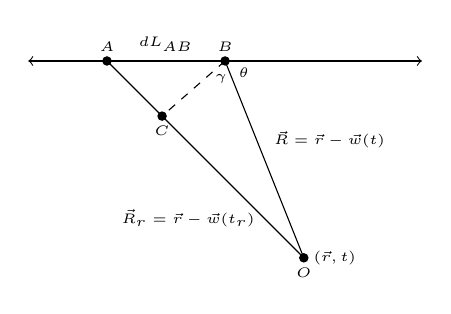
\begin{tikzpicture}[scale=0.5]
        \draw[<->] (-10,0) -- (0,0);
        \filldraw (-8,0) circle(3pt);
        \node[above] at (-8,0) { {\tiny$A$}};
        \node[above] at (-6.5,0) { {\tiny$dL_{AB}$}};
        \filldraw (-5,0) circle(3pt);
        \node[above] at (-5,0) { {\tiny$B$}};
        \node[below] at (-5.1,-0.1) { {\tiny$\gamma$}};
        \node[right] at (-4.9,-0.3) { {\tiny$\theta$}};
        \draw (-8,0) -- (-3,-5);
        \draw (-5,0) -- (-3,-5);
        \filldraw (-3,-5) circle(3pt);
        \filldraw (-6.6,-1.4) circle(3pt);
        \node[left, below] at (-6.6, -1.4) { {\tiny$C$}};
        \draw[dashed] (-5,0) -- (-6.6, -1.4);
        \node[left, below] at (-3,-5) { {\tiny$O$}};
        \node[right] at (-3,-5) {{\tiny$(\vec{r},t)$}};
        \node[right] at (-4,-2) { {\tiny$\vec{R} = \vec{r} - \vec{w}(t)$}};
        \node[left] at (-4,-4) { {\tiny$\vec{R}_r = \vec{r} - \vec{w}(t_r)$}};
    \end{tikzpicture}
    \caption{Picture to explain things}
    \label{5.27.pic}
\end{figure}

Looking at \ref{5.27.pic} under the assumption $A,B$ are close, we note that there is some path length difference in $\vec{R}, \vec{R}_r$ that is given $dL = dL_{AB}\hat{\beta} \cdot \hat{R}_r$. Then we note that there is some difference in travel time $dt'_{AB} = dt_{AB} - \frac{dL}{c}$ the travel time difference between $A,B$ at $(\vec{r},t)$. This shows that information arrives over a shorter time interval, so there's an effective Jacobian $\frac{dt'_{AB}}{dt_{AB}}$ (think of this as analogous to Doppler effect piling up sound waves and increasing frequency, only now we have an increased strength of field), and if we work through the geometry we recover the factor we found above.

Let's do this yet again, still using \ref{5.27.pic} setup but no longer under assumption $A,B$ are close. Define $C$ to be the point that the altitude of $ABO$ hits $AO$, then we find that $AO = \vec{R}_r, BO = \vec{R}$. If we then stare at \eqref{5.27.pots} we note that the denominator of the scaling factor is just $CO$, as the first part is just $AO$ and the second part is exactly the $dL$ that we defined above. But also, noting $\gamma,\theta$ as defined in the picture we find that
\begin{align}
    CO &= BO\sin\gamma\\
    R_r(1 - \vec{b}\cdot \hat{R}_r) &= R\sqrt{1 - \cos^2\gamma}\\
    &= R\sqrt{1 - \beta^2 \sin^2\theta}
\end{align}
and of course we can rewrite the potentials using this factor instead (a bit of trig shows that last step). The cool thing is that the retarded time no longer appears.

Let's now compute the resulting fields. Note that $\pd{}{r_i} = \pd{R_i}{r_i}\pd{}{R_i} = \pd{}{R_i}$ so that $\vec{\nabla}_{r} = \vec{\nabla}_{R}$. Moreover, $\pd{}{t} = -c\vec{\beta} \cdot \vec{\nabla}_R$. Then if we rewrite
\begin{equation}
    R\sqrt{1 - \beta^2 \sin^2\theta} = R\sqrt{1 - \beta^2 \frac{R_{\perp}^2}{R^2}} = \sqrt{R_{\parallel}^2 + \left( 1 - \beta^2 \right)R_{\perp}^2}
\end{equation}
then we can make a motherlode of a bash and find
\begin{align}
    \vec{E}(\vec{r},t) &= -\vec{\nabla}_rV - \pd{\vec{A}}{t}\\
    &= \frac{q}{4\pi\epsilon_0}\left[ -\vec{\nabla}_R + \epsilon_0 \mu_0 c^2 \vec{\beta}\vec{\beta}\cdot \vec{\nabla}_R \right]\frac{1}{\sqrt{R_{\parallel}^2 + \left( 1 - \beta^2 \right)R_{\perp}^2}}\\
    E_{\parallel}(\vec{r},t) &= -\frac{q}{4\pi\epsilon_0}\left( 1 - \beta^2 \right)\pd{}{R_{\parallel}}\frac{1}{\sqrt{R_{\parallel}^2 + \left( 1 - \beta^2 \right)R_{\perp}^2}}\\
    &= -\frac{q}{4\pi\epsilon_0}\left( 1 - \beta^2 \right)\frac{-R_{\parallel}}{\left(\sqrt{R_{\parallel}^2 + \left( 1 - \beta^2 \right)R_{\perp}^2}\right)^3}\\
    \vec{E}_{\perp}(\vec{r},t) &= -\frac{q}{4\pi\epsilon_0}\vec{\nabla}_{R,\perp}\frac{1}{\sqrt{R_{\parallel}^2 + \left( 1 - \beta^2 \right)R_{\perp}^2}}\\
    &= -\frac{q}{4\pi\epsilon_0}\left( 1 - \beta^2 \right)\frac{-R_{\perp}}{\left( \sqrt{R_{\parallel}^2 + \left( 1 - \beta^2 \right)R_{\perp}^2} \right)^3}\\
    \vec{E}(\vec{r},t) &= \frac{q}{4\pi\epsilon_0}\frac{\vec{R}}{R^3}\frac{1-\beta^2}{\left(1 - B^2 \sin^2\theta\right)^{3/2}}
\end{align}

(Goodness copy paste is such a Godsend) We can do similarly for $\vec{B}$ but a little more uglily (Sunil cites the notes) and we get
\begin{align}
    \vec{B}(\vec{r},t) &= \frac{\mu_0}{4\pi}\frac{qc\vec{\beta} \times \vec{R}}{R^3}\frac{1 - \beta^2}{\left( 1 - \beta^2\sin^2\theta \right)^{3/2}}
\end{align}

Curiously $\vec{B} = \frac{1}{c}\vec{\beta} \times \vec{E}$ still! Also, note that the potentials care much more about the ``current'' (extrapolated) position than the retarded position)

Let's go back to the retarded position via $\vec{R} = \vec{R}_r - \vec{\beta}R_r$, then we note that \begin{align}
    \vec{B} &= \frac{1}{c}\vec{\beta} \times \vec{E}\\
    &= \frac{1}{c}\left[ \vec{\beta} + \left( \hat{R}_r - \beta \right) \right] \times \vec{E}\\
    &= \frac{1}{c}\vec{R}_r \times \vec{E}
\end{align}
(We can add the additional term because it is parallel to $\vec{E}$, since $\hat{R}_r - \vec{\beta} \propto \vec{R} \propto \vec{E}$). This then shows us that we can write
\begin{align}
    \vec{E}(\vec{r},t) &= \frac{q}{4\pi\epsilon_0}\frac{\vec{R}_r - \vec{\beta}R_r}{R_r^3}\frac{1 - \beta^2}{\left( 1 - \vec{\beta} \cdot \hat{R}_r \right)^3}\\
    \vec{B}(\vec{r},t) &= \frac{\mu_0}{4\pi}\frac{qc\vec{\beta} \times \vec{R}_r}{R_r^3}\frac{1 - \beta^2}{\left( 1 - \vec{\beta} \cdot \hat{R}_r \right)^3}
\end{align}

Note that all we've done over the course of so long is to take derivatives of the Li\'enerd-Wiechert potentials from \eqref{5.27.pots} with respect to $\vec{r}$ taking $\vec{\beta}$ fixed. However, now we want to have $\vec{\beta}$ varying, so we can just add in the varying $\beta$ terms to our existing results, like product rule.

So we look into how to differentiate $\vec{\beta}$. This is done by writing down
\begin{align}
    t_r &= t - \frac{\abs{\vec{r} - \vec{w}(t_r)}}{c}\\
    c^2\left( t - t_r \right)^2 &= \left[ \vec{r} - \vec{w}(t_r) \right] \cdot \left[ \vec{r} - \vec{w}(t_r) \right]\\
    2c(t-t_r)\left( 1 - \rd{t_r}{t}\Bigg|_{\vec{r}} \right) &= 2\left( \vec{r} - \vec{w}(t_r) \right)\cdot \left( -\rd{\vec{w}}{t_r} \right)\rd{t_r}{t}\Bigg|_{\vec{r}}
\end{align}

Then recalling that $\rd{t_r}{t}\Big|_{\vec{r}} = \frac{1}{1 - \vec{\beta}(t_r) \cdot \hat{R}_r}$ our funky denominator from before, and that $\vec{\nabla}_{\vec{r}} t_r\Big|_t = -\frac{1}{c}\frac{\hat{R}_r}{1 - \vec{\beta}(t_r)\cdot \hat{R}_r}$, then we can take the derivatives of $\vec{\beta}$ and find
\begin{align}
    \pd{\vec{\beta}}{t}\Bigg|_{\vec{r}} &= \pd{\vec{\beta}}{t_r}\Bigg|_{t_r} \pd{t_r}{t}\Bigg|_{\vec{r}} = \pd{\vec{\beta}}{t_r}\frac{1}{1 - \vec{\beta}(t_r) \cdot \hat{R}_r}\\
    \pd{\beta_i}{r_j} &= \pd{\beta_i}{t_r}\Bigg|_{t_r}\pd{t_r}{r_j}\Bigg|_t\\
    \vec{\nabla}_{\vec{r}} \vec{\beta} &= \pd{\vec{\beta}}{t_r}\Bigg|_{t_r}\vec{\nabla}_r t_r\Bigg|_t
\end{align}

This gives us enough to compute the correction terms due to accelerations, which is just given
\begin{align}
    \vec{E} : -\vec{\nabla}_{\vec{r}}V &= -\vec{\nabla}_{\vec{r}}V\Bigg|_{\vec{\beta}} - \frac{1}{4\pi\epsilon_0}\frac{q}{R_r}\frac{1}{\left[ 1 - \vec{\beta} \cdot \hat{R}_r \right]^2}\left( -\vec{\nabla}_{\vec{r}}\left[ \vec{\beta} \cdot \hat{R}_r \right]\Big|_t \right)\\
    &= -\vec{\nabla}_{\vec{r}}V\Bigg|_{\vec{\beta}} - \frac{q}{4\pi\epsilon_0}\frac{\hat{R}_r}{R_r}\frac{1}{\left[ 1 - \vec{\beta} \cdot \hat{R}_r \right]^3}\frac{\hat{R}_r}{c}\cdot \pd{\vec{\beta}}{t_r}\\
    -\pd{\vec{A}}{t}\Bigg|_{\vec{r}} &= -\pd{\vec{A}}{t}\Bigg|_{\vec{B}} - \frac{\mu_0}{4\pi}\frac{qc}{R_r} \frac{1}{\left[ 1 - \vec{\beta} \cdot \hat{R}_r \right]^3} \left[ \left( 1 - \vec{\beta} \cdot \hat{R}_r \right)\pd{\vec{\beta}}{t_r} + \vec{\beta}\left( \hat{R}_r \cdot \pd{\beta}{t_r} \right) \right]
\end{align}

If we then use the ``BAC-CAB'' vector identity, then we can find
\begin{align}
    \vec{E}(\vec{r},t) &= \vec{E}(\vec{r,t)}\Big|_{\vec{\beta}} + \frac{q}{4\pi\epsilon_0}\frac{1}{R_r^3}\frac{\vec{R}_r \times \underbrace{\vec{R}_r - \vec{\beta}R_r}_{\vec{R}} \times \frac{1}{c}\pd{\vec{\beta}}{t_r}}{\left[ 1 - \vec{\beta} \cdot \hat{R}_r \right]^3}\\
    \vec{B}(\vec{r},t) &= \vec{B}(\vec{r,t)}\Big|_{\vec{\beta}}+ \frac{\mu_0 }{4\pi}\frac{qc}{R_r^3}\frac{(R_r - \vec{\beta} \cdot \hat{R}_r)\frac{1}{c}\pd{\vec{\beta}}{t_r}\times \vec{R}_r + \left( \vec{R}_r \cdot \frac{1}{c}\pd{\vec{\beta}}{t_r} \right)\vec{\beta} \times \vec{R}_r}{\left[ 1 - \vec{\beta} \cdot \hat{R}_r \right]^3}
\end{align}

Phew! Let's note that $\vec{B} = \frac{1}{c}\vec{R}_r \times \vec{E} \neq \frac{1}{c}\vec{\beta} \times \vec{E}$ anymore!

We note that the terms tend to go with $\frac{R_r}{c}\pd{\vec{\beta}}{t_r}$, which is on timescale $\frac{t_{light}}{t_{acc}}$, so if the light travel time is short compared to the acceleration timescale then the corrective terms vanish, otherwise they're nonnegligible!

\chapter{5/29/14 --- Radiation of accelerating particles, dipole radiation}

Last time we found the L-W potentials for charge at a fixed $\vec{\beta}$ and then we added in the differential terms of $\vec{\beta}$ to get additional $\vec{E}, \vec{B}$ terms, such that we got
\begin{align}
    \vec{E} - \vec{E}\Bigg|_{\vec{\beta}} &= \frac{q}{4\pi\epsilon_0}\frac{1}{R_r^3}\frac{1}{c}\frac{\vec{R}_r \times \left[ \left( \vec{R}_r - \vec{\beta}R_r \right) \right] \times \pvec{\beta}}{\left[ 1 - \vec{\beta} \cdot \hat{R}_r \right]^3}\Bigg|_{t_r}
\end{align}
where we define $\pvec{\beta}$ to be $\pd{\vec{\beta}}{t_r}$. Then if we compare the magnitude of this acceleration correction we obtain $\frac{R_r  \abs{\pvec{\beta}}}{c}$ which is the ratio of the timescale of light WRT timescale of acceleration. Thus we see that the quasistatic approximation holds when timescale of acceleration falls out. 

Note also $\abs{\vec{E} - \vec{E}\Big|_|\vec{\beta}} \sim R_r^{-1}$, which is different from what we're used to. This is because we differentiated $d\beta$ rather than taking the gradient. This shows that at far distances the radiation term is what is most important! The exact dependences go like $\vec{E}\Big|_{\vec{\beta}} \sim \frac{q}{\epsilon_0}\frac{1}{\gamma^2}\frac{1}{R_r^2}$ and $\vec{E} - \vec{E}\Big|_{\vec{\beta}} \sim \frac{q}{\epsilon_0}\pvec{\beta} \frac{1}{R_r}$.

Lastly recall that $\vec{B} = \frac{1}{c} \hat{R}_r \times \vec{E}$ still holds. Then, noting also that $\vec{E} - \vec{E}\Big|_{\vec{\beta}} \perp \hat{R}_r$ we can compute Poynting vector
\begin{align}
    \vec{S} &= \frac{1}{\mu_0}\left( \vec{E} - \vec{E}\Big|_{\vec{\beta}} \right) \times \left(\vec{B} - \vec{B}\Big|_{\vec{\beta}}\right)\\
    &= \frac{1}{\mu_0}\left( \vec{E} - \vec{E}\Big|_{\vec{\beta}} \right) \times \frac{\hat{R}_r}{c}\times\left(\vec{E} - \vec{E}\Big|_{\vec{\beta}}\right)\\
    &= \frac{1}{c\mu_0}\hat{R}_r \abs{\vec{E} - \vec{E}\Big|_{\vec{\beta}}}^2
\end{align}

Let's first examine the case where acceleration parallel to velocity, then our expression reduces to (since $\vec{\beta} \times \pvec{\beta} = 0$)
\begin{align}
    \vec{E}_{\pvec{\beta}\parallel\vec{\beta}} &= \frac{q}{4\pi\epsilon_0}\frac{1}{R_r}\frac{1}{c}\frac{\hat{R}_r \times \left( \hat{R}_r \times \pvec{\beta} \right)}{\left[ 1 - \vec{\beta} \cdot \hat{R}_r \right]^3}\\
    &= \frac{q}{4\pi\epsilon_0}\frac{1}{R_r}\frac{1}{c}\frac{\pvec{\beta}_{\perp}}{\left[ 1 - \vec{\beta} \cdot \hat{R}_r \right]^3}
\end{align}
with $\pvec{\beta}_{\perp}$ the perpendicular component of $\vec{\beta}$ to $\hat{R}_r$. This shows that we only radiate away from the direction of acceleration.

Let's then define acceleration in the $\hat{z}$ direction, then $\abs{\vec{a}_{\perp}} = a\sin\theta$ with $\vec{a} = c\pvec{\beta}$ then we find
\begin{align}
    \vec{S} &= \frac{\mu_0 q^2}{16 \pi^2} \frac{1}{cR_r^2}\frac{a^2\sin^2\theta}{\left[ 1 - \beta \cos \theta \right]^6} \hat{R}_r\\
    &\sim \frac{1}{R_r^2}\rd{P}{\Omega}
\end{align}
with $\rd{P}{\Omega}$ the power per solid angle. To compute this we note that the power we compute above is radiation in $dt$ but we're interested in the radiation in $dt_r$, which means there's some factor of $\rd{t_r}{t}\Big|_{\vec{\beta}}$ that we're missing, and so we find that the actual field radiated per $\Omega$ is given
\begin{align}
    \rd{P}{\Omega} = \frac{\mu_0}{16\pi^2}\frac{a^2}{c}\frac{\sin^2\theta}{\left[ 1 - \beta \cos\theta \right]^{5}}
\end{align}

He draws a plot that comes straight out of lecture notes. We can integrate $P$ and obtain $P = \frac{\mu_0q^2}{6\pi}\frac{a^2}{c}\gamma^6$ with $\gamma = \frac{1}{\sqrt{1 - \beta^2}}$.

Let's now consider $\pvec{\beta} \perp \vec{\beta}$, and let's fix $\vec{\beta} \propto \hat{z}, \vec{a} \propto \hat{x}$. The algebra is done in Heald and Marion, but we find
\begin{align}
    \rd{P}{\Omega} = \frac{\mu_0 q^2}{16 \pi^2}\frac{a^2}{c}\frac{\left( 1 - \beta \cos\theta \right)^2 - \left( 1 - \beta^2 \right)\sin^2\theta\cos^2\phi}{\left[ 1 - \beta \cos \theta \right]^6}
\end{align}

The classic example of this is a particle in circular motion. We can integrate this over $\Omega$ and obtain $P = \frac{\mu_0}{6\pi}\frac{q^2a^2}{c}\gamma^4$.

For a generic direction of $\pvec{\beta}$ we can extrapolate from our above expression and arrive at the correct expression
\begin{align}
    \rd{P}{\Omega} &= \frac{\mu_0 q^2}{16\pi}\frac{a^2}{c}\frac{\hat{R}_r \times \left[ \left( \hat{R}_r - \vec{\beta} \right)\times \vec{a} \right]}{\left[ 1 - \vec{\beta} \cdot \hat{R}_r \right]^5}\\
    P &= \frac{\mu_0 q^2}{6\pi}\frac{a^2}{c}\frac{1 - \abs{\vec{\beta} \times \vec{a}}^2}{\left( 1 - \beta^2 \right)^3}
\end{align}

Finally we can obtain Larmor's formula for a slowly moving charge by letting $\vec{\beta} \to 0$. Since we can start from either one, we can start from the parallel case ($\vec{\beta}$ no longer has direction in the limit) and we obtain
\begin{align}
    \rd{P}{\Omega} &= \frac{\mu_0q^2}{16\pi^2}\frac{a^2 \sin^2\theta}{cR_r^2}\\
    P &= \frac{\mu_0 q^2}{6\pi}\frac{a^2}{c}
\end{align}

Let's now examine what dipole radiation looks like. This will just be two point charges, and we can take the usual small-distance big-charge limit to get a dipole. We will make the simplifications that $\vec{\beta} = 0$ so we can use the Larmor Formulae, we will assume that the particles make the same $\vec{r}(t)$ trajectory, and that $q\vec{a} \to \ddot{\vec{p}}$. Then we can write down (??)
\begin{align}
    \vec{E}(\vec{r},t) &= \frac{1}{4\pi\epsilon_0}\frac{\vec{r} \times \left( \vec{r} \times \ddot{\vec{p}} \right)}{c^2r}\\
    \vec{B}(\vec{r},t) &= \frac{1}{c}\vec{r} \times \vec{E}\label{5.29.dipoles}
\end{align}
because $\vec{R}_r \to \vec{r}$. Note that we evaluate $\ddot{\vec{p}}$ at $t_r$. Then if we specialize to $\ddot{\vec{p}} \propto \hat{z}$ then we find
\begin{align}
    \vec{E}(\vec{r},t) &= \frac{1}{4\pi\epsilon_0}\frac{\ddot{p}\sin\theta}{c^2r}\hat{\theta}\\
    \vec{B}(\vec{r},t) &= \frac{\mu_0}{4\pi}\frac{\ddot{p}\sin\theta}{cr}\phi\\
    \rd{P}{\Omega} = r^2 \hat{r} \cdot \vec{S} &= \frac{\mu_0}{16 \pi^2}\frac{\ddot{p}\sin^2\theta}{c}\\
    P &= \frac{\mu_0}{6\pi}\frac{\ddot{p}^2}{c}
\end{align}
where the Poynting vector is easily calculated and not shown, and we no longer need the $\rd{t}{t_r}$ factor because $\beta \to 0$. 

Let's now assume some sort of harmonic motion $p(t) = p_0\cos \omega t$, which then gives us
\begin{align}
    \vec{E}(\vec{r},t) &= -\frac{1}{4\pi\epsilon_0}\frac{p_0\omega^2\sin^2\theta}{c^2r}\hat{\theta}\cos\left( \omega\left(t - \frac{r}{c}\right) \right)\\
    \vec{B} &= -\frac{\mu_0}{4\pi}\frac{p_0 \omega^2 \sin^2\theta}{c^2r}\hat{\phi}\cos\left( \omega\left( t - \frac{r}{c} \right) \right)
\end{align}

Note that this does produce some $\vec{\beta}$, but it can be kept small and we're still okay with pretending like our results were accurate. Note also that we do indeed evaluate $\ddot{\vec{p}}$ at $t_r$. Then we can compute
\begin{align}
    \expvalue{\rd{P}{\Omega}} &= \frac{\mu_0}{32\pi^2}\frac{p_0^2\omega^4\sin^2\theta}{c}\\
    \expvalue{P} &= \frac{\mu_0}{12\pi}\frac{p_0^2\omega^4}{c}
\end{align}

Now we can proceed in full generality. Let's first talk about our Fourier transforms really quickly
\begin{align}
    g(t) &= \int\limits_{-\infty}^{\infty}df \;\tilde{g}(f) e^{-i\omega t} & \tilde{g}(t) &= \int\limits_{-\infty}^{\infty}dt\;g(t)e^{i\omega t}\\
    \delta(t) &= \int\limits_{-\infty}^{\infty}dt\;e^{-i\omega t} & \delta(f) &= \int\limits_{-\infty}^{\infty}dt \;e^{-i \omega t} = 2\pi \delta(\omega)
\end{align}

We will also assume that we can sample infinitely well (no upper limit on the transform). Let's now assume that our current and charge distributions are oscillatory
\begin{align}
    \rho(\vec{r},t) &= \rho_0 e^{-i \omega t} & \vec{J}(\vec{r},t) &= \vec{J}_0(\vec{r}) e^{-i \omega t}
\end{align}
then we expect our $\vec{E}$ to have some $e^{-i\omega t}$ dependence as well, as well as $\vec{B}$. Specifically, let's write $\vec{E} = \mathcal{E}\left[ \rho_0, \vec{J}_0 \right]e^{-i\omega t}$ and $\vec{B} = \mathcal{B}\left[ \rho_0, \vec{J}_0 \right]e^{-i\omega t}$ functionals. We can then take Fourier transform
\begin{align}
    \tilde{\rho}(\vec{r},f) &= \int\limits_{-\infty}^{\infty}dt\;\rho(\vec{r},t) e^{-i \omega t} & \tilde{\vec{J}}(\vec{r},t) &= \int\limits_{-\infty}^{\infty}dt\;\vec{J}(\vec{r},t) e^{-i \omega t}
\end{align}
and we can expect $\tilde{\vec{E}}(\vec{r},f) = \mathcal{E}\left[ \tilde{\rho}, \tilde{\vec{J}} \right]$ and same for $\tilde{\vec{B}}$, and we can take inverse Fourier transforms to obtain our actual fields. This is all thanks to linearity.

But then $\expvalue{\vec{S}}$ turns out to also be linear so long as we time average! Let's examine
\begin{align}
    \expvalue{\vec{S}} &= \frac{1}{2\mu_0}\expvalue{\Re\left( \vec{E}^* \times \vec{B} \right)}\\
    &= \frac{1}{2\mu_0} \expvalue{\Re\left[ \int\limits_{-\infty}^{\infty}df_1\;\int\limits_{-\infty}^{\infty}df_2\;e^{i\left( \omega_1 - \omega_2 \right)t}\tilde{\vec{E}}^* \times \tilde{\vec{B}} \right]}
\end{align}

Then we can move the time average inside the frequency integrals
\begin{align}
    &= \frac{1}{2\mu_0}\Re\left[ \int\limits_{-\infty}^{\infty}df_1\;\int\limits_{-\infty}^{\infty}df_2\;\expvalue{e^{i\left( \omega_1 - \omega_2 \right)t}}\tilde{\vec{E}}^* \times \tilde{\vec{B}} \right]\\
    \expvalue{e^{i\omega t}} &= \frac{\delta(f)}{\delta(f=0)}
\end{align}
where we denote $\delta(f=0)$ an infinity (we'll see why later), and we find
\begin{align}
    \expvalue{\vec{S}} &= \frac{1}{\delta(f=0)} \frac{1}{2\mu_0}\Re\left( \int\limits_{-\infty}^{\infty}df\;\tilde{\vec{E}}^*\times \vec{B} \right)
\end{align}

The infinity is just to cancel the fact that the integral is also ininite, whereas usually we would have to integrate over some finite bound. Also, we lost an integral in applying the delta function, so we need the unit back in. 
\chapter{5/31/14 --- Makeup: Radiation from arbitrary source, dipole cases}

I forgot about the makeup lecture, so I will take notes from his lecture notes.

Let's now consider radioation from an arbitrary source distribution. We take Fourier Transforms of the charge and current distributions, whose reconstitution into the full solution was shown by last class to be okay thanks to linearity
\begin{align}
    \rho(\vec{r},t) &= \rho_0(\vec{r}) e^{-i\omega t} & \vec{J}(\vec{r},t) &= \vec{J}_0(\vec{r})e^{-i\omega t}
\end{align}

Let's assume that there are no sources outside some volume $V$. Recall that the retarded potentials are for $t_r = t - \frac{\abs{\vec{r} - \pvec{r}}}{c}$
\begin{align}
    V(\vec{r},t) &= \frac{1}{4\pi\epsilon_0}\int\limits_V d\tau' \frac{\rho(\vec{r},t_r)}{\abs{\vec{r} - \pvec{r}}} & \vec{A}(\vec{r},t) &= \frac{\mu_0}{4\pi}\int\limits_V d\tau' \frac{\vec{J}(\vec{r},t_r)}{\abs{\vec{r} - \pvec{r}}}
\end{align}

Then if we assume harmonic time dependence and no source terms Ampere's Law tells us that
\begin{align}
    \epsilon_0 \mu_0\pd{\vec{E}}{t} = \vec{\nabla} \times \vec{B} \Rightarrow \vec{E} = c^2\frac{i}{\omega}\vec{\nabla} \times \vec{B}
\end{align}
which shows that we need only compute $\vec{A}$. We note that $e^{-i\omega t_r} = e^{-i \omega t}e^{ik\abs{\vec{r} - \pvec{r}}}$ (with $k = \omega/c$), so we can write
\begin{align}
    \vec{A}(\vec{r},t) &= \frac{\mu_0}{4\pi}e^{-i\omega t}\int\limits_V d\tau' \vec{J}_0(\pvec{r}) \frac{e^{ik\abs{\vec{r} - \pvec{r}}}}{\abs{\vec{r} - \pvec{r}}}
\end{align}

Now we make the simplifying assumption that $\abs{\vec{r}} \gg \abs{\pvec{r}}$, i.e. we're evaluating the field far from the distribution, then we can expand
\begin{align}
    \abs{\vec{r} - \pvec{r}} &= \sqrt{r^2 - 2\vec{r} \cdot \pvec{r} + \left( r' \right)^2}\\
    &\approx r - \hat{r} \cdot \pvec{r}\\
    \frac{e^{ik\abs{\vec{r} - \pvec{r}}}}{\abs{\vec{r} - \pvec{r}}} &\approx \frac{1}{r}\left[ 1 + \frac{\hat{r} \cdot \pvec{r}}{r}  \right] \exp\left\{ ik\left( r - \hat{r} \cdot \pvec{r} \right) \right\}\\
    &= \frac{e^{ikr}}{r}\left[ 1 + \frac{\hat{r} \cdot \pvec{r}}{r}  \right]e^{ik\hat{r} \cdot \pvec{r}}\\
    \vec{A} &= \frac{\mu_0}{4\pi}\frac{e^{i(kr - \omega t)}}{r}\int\limits_{V}^{}d\tau'\;\vec{J}_0(\pvec{r}) e^{-ik \hat{r} \cdot \pvec{r}}
\end{align}

Note that we've dropped a few terms that go like $\mathcal{O}(d^2)$ ($d$ is the characteristic size of the source distribution, so $V \sim d^3$), and this only holds in the ``far-field'' approximation, where $d^2/\lambda \ll r$. From this we can calculate the fields, Poynting vector, radiation pattern and total radiated power for harmonic time dependence via
\begin{align}
    \vec{B} &= \vec{\nabla} \times \vec{A} & \vec{E} &= c^2 \frac{i}{\omega}\vec{\nabla} \times \vec{B}\\
    \expvalue{\vec{S}} &= \frac{1}{2\mu_0}\Re\left( \expvalue{\vec{E}^* \times \vec{B}} \right) & \expvalue{\rd{P}{\Omega}} &= r^2 \hat{r} \cdot \expvalue{\vec{S}} & \expvalue{P} &= \int d\Omega \; \rd{P}{\Omega}
\end{align}

If we further make the approximation that $d \ll \lambda$ in addition to $d \ll r$, then we can further expand
\begin{align}
    \vec{A}(\vec{r},t) &= \frac{\mu_0}{4\pi}\frac{e^{i(kr - \omega t)}}{r}\sum\limits_{m=0}^{\infty}\frac{(-ik)^m}{m!}\int\limits_{V}^{}d\tau'\;\vec{J}_0(\pvec{r})\left( \hat{r} \cdot \pvec{r} \right)^m\label{5.31.multipole}
\end{align}

This is the multipole expansion for radiation.

In magnetostatics the $m=0$ term vanished because we assumed steady state currents, in which case $\vec{\nabla} \cdot \vec{J}_0 = 0$ (no net current). Here however we instead throw vector identity and continuity and obtain
\begin{align}
    J_{0,i} e^{-i \omega t} &= \vec{\nabla} \cdot \left( r_i \vec{J}_0 e^{-i \omega t} \right) - r_i\pd{}{t}\left( \rho_0e^{-i \omega t} \right)\\
    &= \vec{\nabla} \cdot \left( r_i \vec{J}_0 e^{-i \omega t} \right) - i\omega r_i\rho_0 e^{-i \omega t}
\end{align}

The first term vanishes by divergence theorem and nothing on boundaries, so we can plug back in and obtain for the $m=0$ term
\begin{align}
    \vec{A}(\vec{r},t) &= \frac{\mu_0}{4\pi}\frac{e^{i(kr - \omega t)}}{r} \int\limits_{V}^{}d\tau'\;\left( -i\omega \right)\rho_0(\pvec{r})\pvec{r}\\
    &= -i\frac{\mu_0}{4\pi}\frac{\omega \vec{p}_0}{r}e^{i\left( kr - \omega t \right)}
\end{align}
which vanishes in the $\omega \to 0$ limit as we expect. 

If we want then the magnetic field due to just this term (I think we're examining only terms up to $r^{-1}$ now) then we must take the curl and drop the term where the curl acts on the $\frac{1}{r}$ because we don't care about $r^{-2}$ behavior, so we obtain
\begin{align}
    \vec{\nabla} \times \left( \vec{p}e^{ikr} \right) &\approx -\vec{p}_0 \times \vec{\nabla} e^{ikr}\\
    &= -\vec{p}_0 \times e^{ikr}\vec{\nabla}(ikr) = -\vec{p}_0 \times e^{ikr}ik\hat{r}\\
    \vec{B}(\vec{r},t) &= \frac{\mu_0}{4\pi}\frac{\omega^2 \hat{r} \times \vec{p}_0}{cr} e^{i(kr - \omega t)}\\
    \vec{E}(\vec{r},t) &= -\frac{1}{4\pi\epsilon_0} \frac{\omega^2 \hat{r} \times \left( \hat{r} \times \vec{p}_0 \right)}{c^2r}e^{i(kr - \omega t)}
\end{align}

Let's now generalize using Fourier Transforms, so we take Fourier decomposition
\begin{align}
    \tilde{\rho}(\vec{r},f) &= \int\limits_{-\infty}^{\infty}dt\;\rho(\vec{r},t) e^{i\omega t} & \tilde{\vec{p}}(f)\left( \vec{r},t \right) &= \int\limits_{V}^{}d\tau'\;\rho(\pvec{r},t) \pvec{r}
\end{align}
whereupon we can treat $\tilde{\vec{p}}(f)e^{-i\omega t}$ as $\vec{p}_0 e^{-i \omega t}$, and then we can sum up the contributions from each $f$. In order words, we can write
\begin{align}
    \tilde{\vec{A}}(\vec{r},f) e^{-i \omega t} &= -i \frac{\mu_0}{4\pi}\frac{\omega \tilde{\vec{p}}(f)}{r}e^{i(kr - \omega t)}\\
    \vec{A}(\vec{r},t) &= \int\limits_{-\infty}^{\infty}df\;\tilde{\vec{A}}(\vec{r},f) e^{-i \omega t}
\end{align}
and then if we recall that factors of $-i\omega$ in the Fourier transform are associated with a derivative, and if we see that $e^{i(kr - \omega t)} \approx e^{-i \omega t_r}$ in the $\abs{\vec{r}}\gg \abs{\pvec{r}}$ limit, then we can write
\begin{align}
    \vec{A}(\vec{r},t) &= \frac{\mu_0}{4\pi}\frac{1}{r}\int\limits_{-\infty}^{\infty}df\;\left[ -i \omega \tilde{\vec{p}}(f) \right]e^{-i \omega t_r}\\
    &= \frac{\mu_0}{4\pi}\frac{\dot{\vec{p}}(t_r)}{r}
\end{align}

Side note, it is much easier to make the Fourier analysis for $\vec{B}, \vec{E}$ than to take the curl/time derivatives of the above expression, because the retarded time is retardedly difficult (ha). This produces the full generalizations in the $d \ll r, d \ll \lambda$ limit
\begin{align}
    \vec{A}(\vec{r},t) &= \frac{\mu_0}{4\pi}\frac{\dot{\vec{p}}(t_r)}{r}\\
    \vec{B}(\vec{r},t) &= -\frac{\mu_0}{4\pi} \frac{\hat{r} \times \ddot{\vec{p}}(t_r)}{cr}\\
    \vec{E}(\vec{r},t) &= \frac{1}{4\pi\epsilon_0} \frac{\hat{r} \times \left( \hat{r} \times \ddot{\vec{p}}(t_r) \right)}{c^2r}
\end{align}

The radiation pattern/power will be the same then as the perfect electric dipole example we did earlier (up from around \eqref{5.29.dipoles}) because the fields are identical, which we can reproduce below (if we take $\vec{p} \propto \hat{z}$) so that
\begin{align}
    \rd{P}{\Omega} &= \frac{\mu_0}{16 \pi^2}\frac{\ddot{p}^2\sin^2\theta}{c} & P &= \frac{\mu_0}{6\pi}\frac{\ddot{p}^2}{c}\\
    \expvalue{\rd{P}{\Omega}} &= \frac{\mu_0}{32 \pi^2}\frac{p_0^2\omega^4\sin^2\theta}{c} & P &= \frac{\mu_0}{12\pi}\frac{p_0^2\omega^4}{c}
\end{align}

Now we get to look at quadrupole radiation! Funsies. We take the $m=1$ term from \eqref{5.31.multipole} which looks like
\begin{align}
    \vec{A}(\vec{r},t) &= \frac{\mu_0}{4\pi}\frac{e^{i(kr - \omega t)}}{r}(-ik)\int\limits_{V}^{}d\tau'\;\vec{J}_0(\pvec{r})\hat{r} \cdot \pvec{r}\label{5.31.M1}
\end{align}
and if we algebra really hard we can show (I swear, he leaves these out in the lecture notes as well)
\begin{align}
    \vec{J}_0(\pvec{r})\hat{r} \cdot \pvec{p} &= \frac{1}{2}\left[ \left( \pvec{r} \times \vec{J}_0 \right) \times \hat{r} \right] + \frac{1}{2}\left[ (\hat{r} \cdot \pvec{r})\vec{J}_0 + \left( \hat{r} \cdot \vec{J}_0 \right)\pvec{r} \right]
\end{align}

We drop the second terms because they're too hard, even though they are of the same magnitude as the terms we keep (\dots inb4 pset problem). We note qualitatively that these are the electric quadrupole terms, while the first terms are the magnetic dipole terms. The first term reminds us of the definition of the magnetic dipole moment $\vec{m}_0 = \int d\tau'\; \frac{\pvec{r} \times \vec{J}_0(\pvec{r})}{2}$, so we can rewrite our vector potential as (as usual, tiny freaking $d$)
\begin{align}
    \vec{A}(\vec{r},t) &= i\frac{\mu_0}{4\pi}\frac{\omega \hat{r} \times \vec{m}_0}{cr}e^{i(kr - \omega t)}
\end{align}

We note that this magnetic dipole radiation is smaller than the electric dipole radiation term by a factor $\frac{m_0}{cp} = kd$ as expected, because in \eqref{5.31.M1} there's an extra $k$ and an extra $\pvec{r}$ inside the integral. 

We can then derive the fields by curling for $\vec{B}$ and using $\vec{E} = c^2(i/\omega)\vec{\nabla} \times \vec{B} = -c\hat{r} \times \vec{B}$ (for harmonic time variation) to obtain
\begin{align}
    \vec{B}(\vec{r},t) &= -\frac{\mu_0}{4\pi}\frac{\omega^2\hat{r} \times \left( \hat{r} \times \vec{m}_0 \right)}{c^2r}e^{i(kr - \omega t)} & \vec{E}(\vec{r},t) = \frac{1}{4\pi\epsilon_0} \frac{\omega^2 \hat{r} \times \left( \hat{r} \times \left( \hat{r} \times \vec{m}_0 \right) \right)}{c^3r}e^{i(kr - \omega t)}
\end{align}

Obviously a triple freaking cross product simplifies, so if we just BAC-CAB the crap out of it we find $\hat{r} \times \hat{r} \times \hat{r} \times \vec{a} = -\hat{r} \times \vec{a}$ so
\begin{align}
    \vec{E}(\vec{r},t) &= -\frac{1}{4\pi\epsilon_0}\frac{\omega^2 \hat{r} \times \vec{m}_0}{c^3r} e^{i(kr - \omega t)}
\end{align}

If we then generalize using Fourier transforms and compute radiation pattern/power for this magnetic dipole case we find
\begin{align}
    \vec{A}(\vec{r},t) &= -i\frac{\mu_0}{4\pi}\frac{\hat{r} \times \dot{\vec{m}}(t_r)}{cr} & \vec{B}(\vec{r},t) &= \frac{\mu_0}{4\pi}\frac{\hat{r} \times \left( \hat{r} \times \ddot{\vec{m}}(t_r) \right)}{c^2r} & \vec{E}(\vec{r},t) &= \frac{1}{4\pi\epsilon_0} \frac{\hat{r} \times \ddot{\vec{m}}(t_r)}{c^3r}\\
    \rd{P}{\Omega} &= \frac{\mu_0}{16\pi^2}\frac{\ddot{m}^2 \sin^2\theta}{c^3} & P &= \frac{\mu_0}{6\pi}\frac{\ddot{m}^2}{c^3}\\
    \expvalue{\rd{P}{\Omega}} &= \frac{\mu_0}{32\pi^2}\frac{m_0^2\omega^4 \sin^2\theta}{c^3} & P &= \frac{\mu_0}{12\pi}\frac{m_0^2 \omega^4}{c^3}
\end{align}

Let's now start relativity. We will follow the standard convention that the inner product for a four-vector is of form $(ct^2) - x_ix_i$.

A four-vector $\mathbf{r}$ is an object whose coordinate representation in a reference frame $F$ comprises four numbers $r^\mu$ that transforms by the Lorentz transformation law
\begin{align}
    \tilde{r}^\mu &= \Lambda^\mu_\nu r^\nu & \Lambda^\mu_\nu = \begin{bmatrix} \gamma & \gamma\beta & 0 & 0\\ \gamma \beta & \gamma & 0 & 0 \\0 & 0 & 1 & 0\\0 & 0 & 0 & 1\end{bmatrix} 
\end{align}

We then seek an invariant connected to $\mathbf{r}$ that is invariant under Lorentz transformations; it turns out that this is 
\begin{align}
    \mathbf{r}^2 &= g_{\mu \nu}r^\mu r^\nu & g_{\mu \nu} &= \begin{bmatrix} 1 & 0 & 0 & 0\\0 & -1 & 0 & 0\\0 & 0 & -1 & 0\\0 & 0 & 0 & -1 \end{bmatrix} \end{align}
with $g$ the \emph{metric}.

More generally, an $n$-th rank tensor $\mathcal{T}$ is an object that has $4^n$ components organized with $n$ indicies and transforms via the Lorentz transformation as $\tilde{T}^{\mu_1\dots\mu_n} = \Lambda^{\mu_1}_{\nu_1} \dots \lambda^{\mu_n}_{\nu_n} T^{\nu_1\dots \nu_n}$. Then a four-vector is a first-rank tensor and the metric is a second-rank tensor. 

We then define the concept of lowering and raising indicies, which is defined via contraction against the metric $r_\mu = g_{\mu\nu}r^{\nu}$ and $T^{\dots\mu_{j-1}\mu_{j+1}\dots}_{\nu_j} = g_{\nu \mu_j}T^{\dots\mu_{j_1}\mu_j\mu_{j+1}\dots}$ and raising can be defined similarly by $g^{\mu \nu} = \left( g^{-1} \right)_{\mu \nu}$. We call raised indicies \emph{contravariant} and lowered indicies \emph{covariant}.

We might then ask how covariant indicies transform, because we've only defined for contravariant indicies. This just looks like $\tilde{r}_\mu = \Lambda_\mu^\lambda r_\lambda$ where $\Lambda_\mu^\lambda = g_{\mu\nu}g^{\sigma\lambda}\Lambda_\sigma^\nu$. 

Then generalizing the gradient turns out to look like $\partial_\mu = \left( \pd{}{r_0}, \pd{}{r_1}, \pd{}{r_2}, \pd{}{r_3} \right)$ and $\partial^\mu = \left( \pd{}{r^0}, \pd{}{r^1}, \pd{}{r^2}, \pd{}{r^3}\right)$, and the Lorentz-invariant derivative $\Box^2 = \partial_\mu \partial^\mu$. 

\chapter{6/3/14 --- Relativity, a.k.a. making sense of electromagnetism}

(I think I took notes too far ahead yesterday) The correct way to generalize the gradient is to require that Taylor expansions work in the right way such that it is covariant. In other words, $S(\mathbf{r} + d\mathbf{r}) = S(\mathbf{r}) + (\mathbf{\nabla}S)_\mu dr^\mu$ with $\mathbf{\nabla}$ the 4-gradient. It then obviously looks like $\mathbf{\nabla}_\mu = \partial_\mu$, and if we raise it using our metric $\partial^\mu = g^{\mu \nu}\partial_\mu$ then we find that $\partial^\mu = \left[ \frac{1}{c}\pd{}{t}, -\pd{}{x}, -\pd{}{y}, -\pd{}{z} \right]$, and the generalized Laplacian looks like $\Box^2 = \partial_\mu \partial^\mu = \frac{1}{c^2}\ptd{}{t} - \nabla^2$.

Let's now try to integrate everything we've had so far into relativity, so we seek a covariant source density $\rho, \vec{J}$. We know that $\tilde{\rho} = \gamma \rho_0$ (there's an argument for why the $\gamma$ belongs here rather than in denominator, but didn't quite catch) how the source charge density transforms, so if we require $\vec{J} = \rho \vec{v} = \rho_0 \gamma \vec{v}$ to transform like a four-vector then we see that $\mathbf{J} = \rho_0 \mathbf{v}$ is the 4-charge density, which transforms like a 4-vector. This is because $J^\mu = \rho_0 v^\mu = \rho_0\gamma(c,\vec{v}) = (\rho,\vec{J})$ with the parentheses vectors.

Then the continuity equation takes a particularly simple form $\partial_\mu J^\mu = 0$, because $\frac{1}{c}\pd{}{t}(c\rho) + \vec{\nabla} \cdot \vec{J} = 0$.

Then we can look at the covariant potentials, if we write $A^\mu = \left( \frac{V}{c}, \vec{A} \right)$ which yields $\Box^2 \mathbf{A} = \mu_0 \mathbf{J}$, our potential wave equations. Moreover, the Lorenz gauge written relatistically just becomes $\partial_\mu A^\mu = 0$, which all of a sudden looks just like the relativistic generalization of the Coulomb gauge

Now let's see how we can rederive the L-W potentials using Lorentz Transformations. Start in the rest frame of particle $F$ such that $V = \frac{1}{4\pi\epsilon_0}\frac{q}{\sqrt{x^2 + y^2 + z^2}}, \vec{A} = 0$. Applying then the Lorentz transformation for a boost in the $\hat{x}$ direction
\begin{align}
    \frac{1}{c}\tilde{V} &= \gamma\left[ \frac{1}{c}V + \beta A_x \right] = \frac{\gamma}{c}V & \tilde{A}_x &= \gamma\left[ A_x + \beta\frac{1}{c}V \right] = \frac{\gamma \beta}{c}V\\
    \tilde{A}_y &= A_y = 0 & \tilde{A}_z &= A_z = 0
\end{align}

Then we want to rewrite in terms of the lab frame coordinates $\tilde{r}^\mu$ while the particle has $r^\mu = (ct, 0, 0, 0)$, so we must apply inverse Lorentz transform
\begin{align}
    ct &= \gamma\left[ c\tilde{t} - \beta \tilde{x} \right] & x &= \gamma\left[ -\beta c\tilde{t} + \tilde{x} \right] & y &= \tilde{y} & z &= \tilde{z}
\end{align}
which gives
\begin{align}
    \tilde{V}(\tilde{r}^\mu) &= \frac{1}{4\pi\epsilon_0}\frac{\gamma q}{\left[ \gamma^2(\beta c\tilde{t} - \tilde{x})^2 + \tilde{y}^2 + \tilde{z}^2 \right]^{1/2}}\\
    &= \frac{1}{4\pi\epsilon_0}\frac{q}{\left[ \left( \tilde{x} - v\tilde{t} \right)^2 - \beta^2 (\tilde{y}^2 + \tilde{z}^2) \right]^{1/2}}
\end{align}

Then if we define $R^2(\tilde{r}^\mu) = (\tilde{x} - v\tilde{t})^2 + y^2 + z^2$ which is just the Cartesian distance from the particle's position $v\tilde{t}$ to the point at which we evaluate the field (in the lab frame) and define $\sin^2\theta = \frac{\tilde{y}^2 + \tilde{z}^2}{R^2}$ (both are just geometric quantities in the lab reference frame) then we find
\begin{align}
    \tilde{V}(\tilde{r}^\mu) &= \frac{1}{4\pi\epsilon_0}\frac{q}{R(\tilde{r}^\mu)}\frac{1}{\left[ 1 - \beta^2 \sin^2\theta \right]^{1/2}}\\
    \tilde{A}_x(\tilde{r}^\mu) &= \beta \tilde{V}(\tilde{r}^\mu)
\end{align}
and of course $\tilde{A}_y = 0, \tilde{A}_z = 0$. So basically, while before we derived everything by solving the wave equations that implied propagation at a finite speed $c$, we can derive everything more simply by noting the wave equations can be written more simply as an operation on a four-vector and then just Lorentz-transforming the four-vector.

Next obvious step is to look at the fields. We define the field (Faraday) tensors to be $F^{\mu \nu} = \partial^\mu A_\nu - \partial_\nu A^\mu$ which also produces $-F^{0j} = F^{j0} = \frac{1}{c}E_j, F^{ij} = -\varepsilon_{ijk}B_j$, which explicitly looks like
\begin{align}
    F^{\mu \nu} &= \begin{bmatrix} 0 & -\frac{E_x}{c} & -\frac{E_y}{c} & -\frac{E_z}{c}\\[10pt]
        \frac{E_x}{c} & 0 & -B_z & B_y\\[10pt]
        \frac{E_y}{c} & B_z & 0 & -B_x\\[10pt]
        \frac{E_z}{c} & -B_y & B_x & 0\end{bmatrix} 
\end{align}
and we can transform this as $\tilde{F}^{\mu \nu} = \Lambda^\mu_\lambda\Lambda^\nu_\sigma F^{\lambda \sigma}$. 

Apparently, lowered/raised latin indicies are the same, so $E_i = E^i, B_i=B^i, \beta_i = \beta^i, \delta_{jk} = \delta^j_k$. This then gives us
\begin{align}
    \tilde{E}_j &= -c\tilde{F}^{0j} = -c\Lambda^0_\lambda \Lambda^j_\sigma F^{\lambda\sigma}\\
    &= \left[ \Lambda^0_0\Lambda^j_0F^{00} + \Lambda^0_0\Lambda^j_kF^{0k} + \Lambda^0_k\Lambda^j_0 F^{k0}+ \Lambda^0_k \Lambda^j_l F^{kl} \right]\\
    \dots &= \gamma E_j + \left( 1-\gamma \right)\frac{\beta_j\beta_k}{\beta^2}E_k - \gamma v_k\varepsilon_{jkl}B_l\\
    \tilde{B}_j =\dots &= \gamma B_j + \left( 1-\gamma \right)\frac{\beta_j\beta_k}{\beta^2}B_k + \frac{\gamma}{c^2}\varepsilon_{jl}v_kE_l
\end{align}
where we can bash some algebra (taking advantage of antisymmetry of $F$) to obtain these expressions for $\tilde{E}$ and same for $\tilde{B}$. If we write these out as the fields we find
\begin{align}
    \tilde{\vec{E}} &= \gamma \vec{E} + \left( 1 - \gamma \right)\hat{\beta}\left( \hat{\beta} \cdot \vec{E} \right) - \gamma\vec{v} \times \vec{B}\\
    \tilde{\vec{B}} &= \gamma \vec{B} + \left( 1-\gamma \right)\hat{\beta}\left( \hat{\beta} \cdot \vec{B} \right) + \frac{\gamma}{c^2}\vec{v} \times \vec{E}
\end{align}
which is still a bit too generic, but if we define then $\vec{E}_{\parallel} = \hat{\beta}(\hat{\beta} \cdot \vec{E}), \vec{E}_{\perp} = \vec{E} - \vec{E}_{\parallel}$ and similarly for $\vec{B}$ we find that
\begin{align}
    \tilde{E}_{\parallel} &= E_{\parallel} & \tilde{E}_\perp &= \gamma\left[ \vec{E}_{\perp} - \vec{v} \times \vec{B}_\perp \right]\\
    \tilde{B}_{\parallel} &= B_{\parallel} & \tilde{B}_\perp &= \gamma\left[ \vec{B}_\perp + \frac{1}{c^2} \vec{v} \times \vec{E}_\perp\right]
\end{align}

We can read off the inductive term above and the Lorentz contractions. This is really cool because just figuring out how this field tensor transforms immediately pops out all of the transformation laws for the fields, rather than having to worry about special cases or transforming source densities.

Let's now look at the field of a moving point charge. In the rest frame we have $\vec{E} = \frac{q}{4\pi\epsilon_0}\frac{\hat{r}}{r^2}, \vec{B} = 0$. Then if we fix $\vec{v} = v\hat{x}$ then we find
\begin{align}
    \tilde{E}_x(\tilde{r}^\mu) &= \tilde{E}_\parallel = E_x = \frac{1}{4\pi\epsilon_0}\frac{qx}{r^3}\\
    \tilde{B}_x(\tilde{r}^\mu) &= \tilde{B}_\parallel = B_x = 0\\
    \tilde{\vec{E}}_{yz}(\tilde{r}^\mu) &= \gamma\left( \vec{E}_{\perp} - \vec{v} \times \vec{B}_\perp \right) = \frac{1}{4\pi\epsilon_0}\frac{\gamma q}{r^3} \left( y\hat{y} + z\hat{z} \right)\\
    \tilde{\vec{B}}_{yz} &= \tilde{\vec{B}}_{\perp} = \gamma\left[ \vec{B}_{\perp} + \frac{1}{c^2}\vec{v} \times \vec{E}_\perp \right] = \frac{1}{c^2} \vec{v} \times \tilde{E}_\perp
\end{align}

Then we need to go to the lab frame, so we Lorentz transform $ct = \gamma \left[ c\tilde{t} - \beta \tilde{x} \right], x = \gamma\left[ -\beta c\tilde{t} + \tilde{x} \right]$ and we obtain (skipping some steps)
\begin{align}
    \tilde{E}(\tilde{r}^\mu) &= \frac{1}{4\pi\epsilon_0} \frac{\gamma q \vec{R}(\tilde{r}^\mu)}{\gamma^2\left[ \left\{ (\tilde{x} - v\tilde{t})^2 + y^2 + z^2 \right\} - \beta^2\left( \tilde{y}^2 + \tilde{z}^2 \right) \right]^{3/2}}\\
    &= \frac{1}{4\pi\epsilon_0}\frac{q\vec{R}(\tilde{r}^\mu)}{\left[ R(\tilde{r}^\mu) \right]^3}\frac{1 - \beta^2}{\left[ 1 - \beta^2\sin^2\theta \right]^{3/2}}\\
    \tilde{\vec{B}} &= \frac{1}{c}\vec{\beta} \times\tilde{\vec{E}}
\end{align}
with our usual definitions. 

Let's then look at invariants of the EM field. We can lower the indicies $F_{\mu \nu}$ and it turns out that just all the signs are flipped. Then we can compute and find $F_{\mu \nu}F^{\mu \nu} = -\frac{2}{c^2}\vec{E}\cdot \vec{E} + 2\vec{B} \cdot \vec{B}$ (note this is not matrix multiplication, the indicies are matched), so we find that $E^2 - c^2B^2$ is a Lorentz invariant. Note this is not the energy density! The energy density forms a four-vector with the Poynting vector and transforms under Lorentz transform.

For more invariants we define a dual tensor $G^{\mu \nu} = \frac{1}{2}\varepsilon^{\mu \nu \lambda \sigma}F_{\lambda \sigma}$ with $\varepsilon^{\mu \nu \lambda \sigma}$ the expected 4D generalization of the Levi-Civita. It turns out that $G$ just flips all the $B$s and $E$s like
\begin{align}
    F^{\mu \nu} &= \begin{bmatrix} 0 & -B_x & -B_y & -B_z\\[10pt]
        B_x & 0 & -\frac{E_z}{c} & \frac{E_y}{c}\\[10pt]
        B_y & \frac{E_z}{c} & 0 & -\frac{E_x}{c}\\[10pt]
        B_z & -\frac{E_y}{c} & \frac{E_x}{c} & 0\end{bmatrix} 
\end{align}

Then if we examine $F_{\mu \nu}G^{\mu \nu} = -\frac{4}{c}\vec{E} \cdot \vec{B}$ so $\vec{E} \cdot \vec{B}$ is also Lorentz-invariant.

We can then look at Maxwell's equations, which can be written
\begin{align}
    \partial_\mu F^{\mu \nu} &= \partial_\mu \partial^\mu A^\nu - \partial_\mu \partial^\mu A^\mu = \Box^2 A^\nu + 0 = \mu_0 J^\nu\\
    \partial_\mu F^{\mu \nu} &= \mu_0 J^\nu A\label{6.3.inhomo}\\
    \partial_\mu G^{\mu \nu} &= \frac{1}{2}\partial_\mu \varepsilon^{\mu \nu \lambda \sigma}\left( \partial_\lambda A_\sigma - \partial_\sigma A_\lambda \right) = \partial_\mu \varepsilon^{\mu \nu \lambda \sigma}\partial_\lambda A_\sigma = 0 \label{6.3.homo}
\end{align}
where we note the antisymmetry kills the one-half and then antisymmetry means that the $\varepsilon$ will cancel equal terms and stuff vanishes. The first equation \eqref{6.3.inhomo} encodes the inhomogeneous Maxwell Equations and the second equation \eqref{6.3.homo} encodes the homogeneous Maxwell Equations.

Let's now figure out how the Lorentz force can be written in a covariant way. Let's first look at the instantaneous rest frame of the particle where we find $\rd{}{t}\left( m\rd{x^i}{t} \right) = qE^i = qcF^{i0}$. Then if we want to generalize this we expect the term in parentheses to go to the four-momentum $p^\mu = mv^\mu = m\gamma(c,\vec{v})$ again paretheses denoting vector. Moreover, the time derivative doesn't transform nicely, so let's take derivative $\rd{}{\tau}, \tau^2 = c^2t^2 - r^2$ the proper time. Lastly we guess that $c \to v_\nu$. So our guesstimate looks like
\begin{align}
    \rd{}{\tau}p^\mu &= qF^{\mu \nu}v_\nu
\end{align}

If we then look at the space component we find
\begin{align}
    \rd{t}{\tau}\rd{p^i}{t} &= q\left( \frac{E^i}{c}\gamma c - \varepsilon_{ijk}B_k\left( -\gamma \vec{v} \cdot \hat{r}_j \right) \right)\\
    \gamma \vec{F} \cdot \hat{r}_i &= \gamma q\left( E_i + \left( \vec{v} \times \vec{B} \right)_i \right)\\
    \vec{F} \cdot \hat{ r}_i &= q\left( \vec{E} + \vec{v} \times \vec{B} \right)
\end{align}
where we identify $\rd{p^i}{t}$ with the $i$th component of the $\vec{F}$, and $\rd{t}{\tau} = \gamma$.

Then looking at the zeroth component we find ($p^0 = \gamma mc$)
\begin{align}
    \rd{t}{\tau}\rd{}{t}\gamma mc &= q\left( F^{00}v_0 + F^{0i}v_i \right)\\
    \gamma \rd{}{t}\gamma mc &= \gamma q \frac{E_i}{c} \vec{v} \cdot \hat{r}_i\\
    \rd{}{t}U &= q\vec{v} \cdot \vec{E}
\end{align}
so only the electric field can change the energy of the particle.

Lastly we want to take the Maxwell Stress tensor to covariant form, the Maxwell Energy-Momentum Tensor. Since there's only two indicies, we're limited in our choice, and we will choose
\begin{align}
    T^{\mu \nu} &= \frac{1}{\mu_0\left[ F^\mu_\lambda F^{\lambda \nu} + \frac{1}{4}g^{\mu \nu}F_{\lambda \sigma}F^{\lambda \sigma} \right]}\\
    T^{00} &= \frac{\epsilon_0}{2}\left( E^2 + c^2B^2 \right) = U\\
    T^{ij} &= \epsilon_0 \left( -E_iE_j - c^2B_iB_j + \frac{\delta^{ij}}{2}\left( E^2 + c^2B^2 \right) \right) = -\mathbf{T}\\
    T^{0i} &= -\frac{1}{\mu}\frac{1}{c}\varepsilon_{ijk}E_jB_k = -\frac{1}{c}S_i
\end{align}
where we find that $\mathbf{T}$ the Maxwell stress tensor and $S_i$ the Poynting vector just pop out of this covariant $T^{\mu \nu}$. We can also write down the fairly ugly angular momentum tensor $M^{\mu \nu \sigma} = T^{\mu \nu}x^\sigma - T^{\mu \sigma}x^\nu$.

We can write down a conservation law for $T^{\mu \nu}$, which comes from taking the divergence 
\begin{align}
    \partial_\mu T^{\mu \nu} &= \frac{1}{\mu}\left[ \left( \partial_\mu F^\mu_\lambda \right)F^{\lambda \nu} + F^{\mu \lambda}\partial_\mu F^{\lambda \nu} + \frac{1}{2}\partial^\nu\left[ F_{\lambda \sigma}F^{\lambda \sigma} \right] \right]\\
    \dots &= \frac{1}{\mu}\left[ \mu_0 J_\lambda F^{\lambda \nu} + 0 \right]\\
    &= -F^{\nu \lambda}J_\lambda
\end{align}
where the second terms vanish because we eventually hit $\partial_\mu G^{\mu \nu} = 0$. If we then look at the time and space components respectively we find
\begin{align}
    \pd{U}{t} - \vec{\nabla} \cdot \vec{S} &= \vec{J} \cdot \vec{E} = \pd{U_{mech}}{t}\\
    \pd{\vec{g}}{t} + \vec{\nabla} \cdot \mathbf{T} &= \left[ \rho \vec{E} + \vec{J} \times \vec{B} \right] = \pd{p_{mech}}{t}
\end{align}
so we recover our conservation equations too. 
\chapter{6/5/14 --- Final Review Session!}

Last year's problems included 
\begin{enumerate}
    \item EM waves in free space (Poynting vector, circular polarization)
    \item EM waves incident on conductor
    \item Loss in TEM mode for imperfect conductor (similar to PS7 strip line problem)
    \item Transmission line with frequency-dependent conductivity
    \item Relativistic motion of a charged particle in a $\vec{B}$ field
    \item Radiation from a bouncing mass. There were five problems per grad/ugrad exam. 
\end{enumerate}
We will do the problems as the class determines. Note that problems on the exam will not be nearly as algebra-intensive as the psets for obvious time reasons, and we will notice this as we go through the problems. Class likes the later problems, we'll go in backwards order.

We start with 6. \emph{Consider a mass $m$ carrying charge $q$ dropped from height $h$ to fall under gravity $g$ and bounces elastically. Find $\Delta h$ between first and second bounce due to loss of energy by radiation. Assume $\Delta h \ll h$.} In case this wasn't evident from before, radiation damping is a real thing, i.e. particle dissipation via radiation should slow particle down.

So the power emitted is given by our earlier studies $\frac{\mu_0}{6\pi}\frac{q^2a^2}{c^2} = \frac{\mu_0}{6\pi}\frac{\ddot{p}^2}{c}$. For us, the dipole moment is just $qh$ with $h$ the height defined with respect to some origin, and so $\ddot{p} = q\ddot{h} = qg$ (note that the origin choice doesn't matter; alternatively, $a=g$ acceleration, so use the former formula for accelerating charge rather than dipole). Assuming then $\Delta h \ll h$ we can equate $mg\Delta h = P\Delta t = P\left(2\sqrt{\frac{2h}{g}}\right)$ (kinematics tells us how long it takes to fall, and multiply by $2$ because it has to go back up). We then compute
\begin{align}
    \Delta h &= \frac{\mu_0}{3\pi}\frac{1}{mc}\sqrt{2gh}
\end{align}

Note that in solving this problem we're ignoring the accelerative period, which since we treat acceleration as a delta function is a very very very gracious simplification (this wasn't mentioned in the problem on the exam!). The slightly more complicated problem is if $\Delta h$ is no longer small, in which case we would have to include the slowdown of the particle as it is falling. Not particularly more complicated.

Next problem is problem 5. \emph{Consider the motion of a relativistic particle in a constant $\vec{B} = B_0\hat{z}$. Show that this yields a helix $\phi \propto z$ even in the relativistic calculation.}

Let's do the nonrelativistic calculation first. We decompose $\vec{v} = v_{\parallel}\hat{z} + \vec{v}_{\perp}$. Then we write down that $m\dot{\vec{v}} = q\vec{v}_{\perp} \times \vec{B}$, we can work some vector stuff out and find $\frac{mv_{\perp}^2}{R} = qv_{\perp}B, v_{\perp} = \frac{qBR}{m}$ for $R$ the radius of the orbit. Then we find that since the particle goes in a circle $\phi \propto t, \propto z$ because $z = v_{\parallel}t$, which produces a helix.

Relativistically, we exhibit $\rd{}{t}(\gamma m\vec{v}) = q\vec{v} \times \vec{B}$. We know that $\vec{B}$ does no work so $\abs{\vec{v}}$ is constant, and so is $\gamma$ and we can pull it out and obtain
\begin{align}
    \gamma m\rd{\vec{v}}{t} = q\vec{v}_{\perp}\times \vec{B}
\end{align}
at which point we have the same calculation as before but with this extra $\gamma$; this produces $\frac{v_{\perp}^2}{R} = \frac{qB}{m\gamma}v_{\perp}, v_{\perp} = \frac{qB_0R}{m\gamma}$. This still shows that we have helical motion.

Next we can do problem 4. \emph{We discussed in class the Drude model for quasistatic conductivity which gave $\sigma = \frac{ne^2\tau}{m}, \tau = \frac{\lambda}{2v_{th}}$ for $v_{th}$ thermal velocity, and $\lambda$ mean free path. In the non-quasistatic limit, $\sigma = \frac{ne^2\tau/m}{1 - i\omega \tau}$, so $R = R_0(1 - i\omega \tau)$. Find $v$ propagating velocity and show that propagation even if $\mathcal{L} \to 0$.}

We see that the non-quasistatic limit applies when $\omega \gg \frac{1}{\tau}$, or when the period of the field oscillations is larger than the meantravel time of the electrons. Otherwise, we start by setting up our differential equations for our transmission line the same way as in the homework
\begin{align}
    \ptd{I}{z} &= \mathcal{LC}\ptd{I}{t} + 2\mathcal{RC}\pd{I}{t}\\
    \ptd{V}{z} &= \mathcal{LC}\ptd{V}{t} + 2\mathcal{RC}\pd{V}{t}
\end{align}

Assuming then harmonic time dependence we plug in and find
\begin{align}
    \tilde{k}^2 I_0e^{-i\omega t} &= \left[ \left( \mathcal{L} + 2R_0\tau \right)C\omega^2 + 2\mathcal{R_0C}i\omega \right]I_0e^{-i\omega t}
\end{align}

This equation then looks exactly like the equation we had for EM waves in conductors, so we make the substitution $\mu \epsilon \to \left( \mathcal{L} + 2R_0\tau \right)\mathcal{C}, \sigma \mu \to 2\mathcal{R}_0\mathcal{C}$. Then we can plug into the expressions that we had found for $k,\kappa$ using these new expressions and we find
\begin{align}
    k &= \omega \sqrt{\frac{(\mathcal{L} + 2\mathcal{R}_0 \tau)\mathcal{C}}{2}}\left[ \sqrt{1 + \left( \frac{2\mathcal{R}_0\mathcal{C}}{(\mathcal{L} + 2\mathcal{R}_0 \tau)\mathcal{C}\omega} \right)^2} + 1 \right]^{1/2}
\end{align}
and $v = \omega/k$. We then note that for $\mathcal{L} \to 0$ propagation still occurs because of the $2\mathcal{R}_0\tau$.

Next is problem 2. \emph{Consider an interface beteen vacuum and conductor with $\sigma, \epsilon, \mu$. Show for $\phi$ the phase shift of the reflected wave that $\tan \phi = \frac{2k_t/k_0}{(k_0^2 + \kappa_t^2)/k_0^2 - 1}$ for some $k_0$ TBD, that $\tan \phi \to 0$ for $\sigma \to \infty$ and so that $\phi = 0,\pi$ in that limit. Assume normal incidence}. Call $\tilde{k}_t = k_t + i\kappa_t$ propagation in the conductor.

This is just a BVP, we learned the explicit form $\frac{\tilde{E}_{0,r}}{\tilde{E}_{0,i}} = \frac{1 - \tilde{\beta}}{1 + \tilde{\beta}}$. For us
\begin{align}
    \tilde{\beta} &= \frac{\mu_1}{\mu_2}\frac{v_1}{\omega}(k_t + i\kappa_t) = \frac{\mu_0}{\mu}\frac{c}{\omega}(k_t + i\kappa_t) = \frac{k_t + i\kappa_t}{k_0}
\end{align}
where we define $k_0$. Then we plug into the reflection coefficient and we obtain
\begin{align}
    \frac{1 - \tilde{\beta}}{1 + \tilde{\beta}} &= \frac{\left( 1 - \frac{k_t}{k_0} + i\frac{\kappa_t}{k_0} \right)}{\left( 1 + \frac{k_t}{k_0} \right) + i\frac{\kappa_t}{k_0}}\\
    &= \frac{\left( 1 - \frac{k_t^2 + \kappa_t^2}{\omega^2} \right) - 2i\frac{k_t}{k_0}}{\mathbb{R}\text{ stuff}}\\
    \tan \phi &= \frac{-2\frac{k_t}{k_0}}{1 - \frac{k_t^2 + \kappa_t^2}{k_0^2}}
\end{align}

Then in the limit that $\sigma \to \infty$ we find that $k_t + i\kappa_t \to \frac{1}{\delta} = \sqrt{\frac{\sigma \mu \omega}{2}} \to \infty$, and since $k_0$ is still finite we get that $\phi \to \pi$. 

Next is problem 1. \emph{There are two cases of EM waves given below. For each pair, calculate $\vec{S}, \expvalue{U}$ and relate them to circularly polarized waves.}
\begin{align}
    \vec{E}_A(\vec{r},t) &= E_0\sin \omega t\left( \hat{x}\sin kz + \hat{y\cos kz} \right)\\
    \vec{B}_A(\vec{r},t) &= \frac{E_0}{c}\cos \omega t\left( \hat{x}\sin kz + \hat{y\cos kz} \right)\\
    \vec{E}_B(\vec{r},t) &= E_0\cos kz\left( \hat{x}\cos \omega t - \hat{y}\sin \omega t \right)\\
    \vec{B}_B(\vec{r},t) &= -\frac{E_0}{c}\sin kz\left( \hat{x}\cos \omega t - \hat{y}\sin \omega t \right)
\end{align}

Note that we have $\vec{E} \parallel \vec{B}$ which produces $\vec{S} = 0$ in both cases. We then find $\expvalue{U} = \frac{1}{2}\epsilon_0 E_0^2$ for both cases. That's actually it for ths part.

If we then want to relate them to circular polarization, then we have to rewrite these into $kz - \omega t$ dependences, because we're used to seeing how propagating waves combine while these look much more like standing waves. This goes
\begin{align}
    \vec{E}_A &= \frac{E_0}{2}\left\{ \hat{x}\left[ \cos(kz - \omega t) - \cos (-kz - \omega t) \right] + \hat{y}\left[ -\sin(kz - \omega t) - \sin(-kz - \omega t) \right] \right\}
\end{align}
and simlilarly for the rest. The way to figure this out is just that we have four total propagating waves and then figure out the coefficients to reduce to the forsm we were given. Regrouping the terms in terms of propagation direction we get
\begin{align}
    \vec{E}_A &= \frac{E_0}{2}\left\{ \left[\hat{x} \cos(kz - \omega t) - \hat{y}\sin(kz - \omega t)\right] - \left[\hat{x}\cos (kz + \omega t) - \hat{y}\sin(kz + \omega t)\right]\right\}
\end{align}
and we see that this wave is a superposition of a positive helicity, left circularly polarized (first term) wave, and a negative helicity, right cicularly polarized wave (second term). There is a phase shift by a $\pi$ as is evident from the $-$ sign. The second case has phase difference $0$ instead, worked the exact same way. 

\end{document}
